\documentclass[12pt,a4paper,oneside,openany]{report}
\usepackage[utf8]{inputenc}
\usepackage[T1]{fontenc}
\usepackage{mathptmx}
\usepackage[left=3cm, right=2cm, top=2.5cm, bottom=2cm]{geometry}
\usepackage{setspace}
\setstretch{1.5}
\usepackage{amsmath,amssymb,amsthm}
\usepackage{graphicx}
\graphicspath{{figures/}}
\usepackage{booktabs,longtable,array,multirow,caption}
\usepackage[table]{xcolor}
\usepackage{listings}
\lstset{language=Python,basicstyle=\ttfamily\small,
  keywordstyle=\color{blue},commentstyle=\color{gray},
  stringstyle=\color{orange},breaklines=true,frame=single,
  numbers=left,numberstyle=\tiny\color{gray},xleftmargin=15pt,
  extendedchars=true,inputencoding=utf8}
\usepackage{fancyhdr}
\usepackage{enumitem}
\usepackage{pdfpages}
\usepackage{subcaption}
\usepackage{float}
\pagestyle{fancy}
\fancyhf{}
\fancyfoot[C]{\thepage}
\def\headrulewidth{0pt}
\def\footrulewidth{0pt}
\fancypagestyle{plain}{\fancyhf{}\fancyfoot[C]{\thepage}\def\headrulewidth{0pt}}
\usepackage[numbers]{natbib}
\usepackage{url}
\bibliographystyle{unsrt}
\usepackage[hidelinks,bookmarks=true,bookmarksnumbered=true,
  pdfencoding=auto]{hyperref}
\hypersetup{
  pdftitle={Quantifying Privacy Risk in Token-Based CBDC: A Normalised Metadata De-Anonymization Framework for Nepal},
  pdfauthor={Prashish Dahal},
  pdfsubject={Bachelor's Project Report, KU School of Science},
  pdfkeywords={CBDC, privacy, blockchain, de-anonymization, Nepal}
}
\pdfstringdefDisableCommands{%
  \def\Rnorm{R\_norm}%
  \def\Rraw{R\_raw}%
  \def\Rmax{R\_max}%
  \def\mathrm#1{#1}%
  \def\lambda{lambda}%
  \def\binom#1#2{C(#1,#2)}%
}
\newtheorem{theorem}{Theorem}[chapter]
\newtheorem{definition}{Definition}[chapter]
\newtheorem{proposition}{proposition}[chapter]
\newcommand{\Rnorm}{R_{\mathrm{norm}}}
\newcommand{\Rraw}{R_{\mathrm{raw}}}
\newcommand{\Rmax}{R_{\mathrm{max}}}
\AtBeginDocument{%
  \renewcommand{\contentsname}{\centering TABLE OF CONTENTS}%
  \renewcommand{\listfigurename}{\centering LIST OF FIGURES}%
  \renewcommand{\listtablename}{\centering LIST OF TABLES}%
}
\begin{document}
\pagenumbering{roman}
\pagestyle{plain}
\begin{titlepage}
\thispagestyle{empty}
\begin{center}

\vspace*{0.5cm}

{\large \textbf{Quantifying Privacy Risk in Token-Based CBDC:}}\\[0.2em]
{\large \textbf{A Normalised Metadata De-Anonymization}}\\[0.2em]
{\large \textbf{Framework for Nepal}}\\[1.5cm]

{\large A FINAL YEAR PROJECT}\\[1cm]

{\large SUBMITTED IN}\\[0.3cm]
{\large PARTIAL FULFILLMENT OF THE REQUIREMENTS FOR}\\[0.3cm]
{\large THE BACHELOR'S DEGREE IN COMPUTATIONAL MATHEMATICS}\\[1cm]

{\large BY}\\[0.5cm]

{\large Prashish Dahal}\\[1.5cm]


\includegraphics[width=3cm]{ku_logo}\\[1cm]

{\large DEPARTMENT OF MATHEMATICS}\\[0.5cm]
{\large SCHOOL OF SCIENCE}\\[0.5cm]
{\large KATHMANDU UNIVERSITY}\\[0.5cm]
{\large DHULIKHEL, NEPAL}\\[0.8cm]

{\large May 2026}

\end{center}
\end{titlepage}
\newpage
\begin{center}
{\Large \textbf{DECLARATION}}\\[1cm]
\end{center}

\noindent
I, \textbf{Prashish Dahal}, hereby declare that the work contained herein is
entirely my own, except where stated otherwise by reference or
acknowledgement, and has not been published or submitted elsewhere,
in whole or in part, for the requirement of any other degree or
professional qualification. Any literature, data or works done by
others and cited within this work has been given due acknowledgement
and listed in the reference section.

\vspace{3cm}
\begin{flushleft}
\rule{6cm}{0.4pt}\\
Prashish Dahal\\[0.5cm]
Date: \rule{4cm}{0.4pt}
\end{flushleft}
\newpage
\begin{center}
{\Large \textbf{CERTIFICATION}}\\[1cm]
\end{center}

\noindent
This work entitled \textbf{``Quantifying Privacy Risk in Token-Based CBDC: A
Normalised Metadata De-Anonymization Framework for Nepal''} is carried out
under our supervision for the specified entire period satisfactorily, and is
hereby certified as original work done by \textbf{Prashish Dahal} in partial
fulfillment of the requirements for the Bachelor's degree in Computational
Mathematics, Kathmandu University, Dhulikhel, Nepal.

\vspace{1.5cm}

\noindent
\begin{minipage}[t]{0.45\textwidth}
\raggedright
\rule{5.5cm}{0.4pt}\\[0.3cm]
\textbf{Dr. Gokul K.C.}\\[0.2cm]
Associate Professor\\
Department of Mathematics\\
School of Science\\
Kathmandu University\\[0.5cm]
Date: \rule{3.5cm}{0.4pt}
\end{minipage}
\hfill
\begin{minipage}[t]{0.45\textwidth}
\raggedright
\rule{5.5cm}{0.4pt}\\[0.3cm]
\textbf{Dr. Samir Shrestha}\\[0.2cm]
Associate Professor\\
Department of Mathematics\\
School of Science\\
Kathmandu University\\[0.5cm]
Date: \rule{3.5cm}{0.4pt}
\end{minipage}

\vspace{2cm}

\noindent
\textbf{APPROVED BY:}\\

\noindent
I hereby declare that the candidate qualifies to submit this work as a Bachelor's
final year project to the Examination Committee.

\vspace{1.5cm}
\noindent
\rule{5.5cm}{0.4pt}\\[0.3cm]
\textbf{Prof. Dr. Rabindra Kayastha}\\[0.2cm]
Head of the Department\\
Department of Mathematics\\
School of Science, Kathmandu University\\[0.5cm]
Date: \rule{3.5cm}{0.4pt}
\newpage\thispagestyle{empty}
\chapter*{Abstract}
\addcontentsline{toc}{chapter}{Abstract}
\vspace{0.5cm}

Central Bank Digital Currencies (CBDCs) promise to modernise
payment infrastructure while extending financial inclusion to
unbanked populations. However, the transition from physical cash
to digital tokens introduces a critical privacy challenge: every
transaction leaves a metadata trail that can expose citizens to
re-identification even when no names are recorded. This risk is
particularly significant in Nepal, where the Nepal Rastra Bank
(NRB) is actively exploring a domestic token-based CBDC for
deployment across diverse geographic and demographic contexts.

Existing approaches to CBDC privacy comparison are qualitative in
nature, offering no formal metric by which policymakers can
measure, compare, or regulate metadata de-anonymization risk
across different cryptographic scheme choices. This thesis
addresses that gap by developing a formal, normalised privacy risk
model grounded in information-theoretic principles.

The model introduces three core components: a single-attribute
uniqueness score $s(a_i)$, a pairwise interaction coefficient
$\lambda_{ij}$ that captures amplification effects between
attribute combinations, and a normalised risk score
$R_{\mathrm{norm}} = R_{\mathrm{raw}} / R_{\mathrm{max}}$,
where $R_{\mathrm{max}}(m) = m + \binom{m}{2}$ is derived from
first principles as the proven theoretical upper bound. The model
is applied to six cryptographic schemes --- Plain Hash Token,
Blind Signature, Hybrid Scheme, Ring Signature, Stealth Address,
and ZKP Token --- across seven metadata attributes, including two
Nepal-specific fields: payment channel and transaction zone.

Results demonstrate that the six schemes form a clean,
non-overlapping risk ladder from $R_{\mathrm{norm}} = 0.317$
(Plain Hash Token) to $R_{\mathrm{norm}} = 0.035$ (ZKP Token).
Population scale provides no meaningful privacy improvement for
weak schemes, with Plain Hash Token at $N = 100{,}000$ remaining
$5.5\times$ riskier than ZKP Token. Nepal's demographic clustering
provides passive privacy protection at domestic scale. Statistical
validation across 30 random seeds confirms the scheme ranking is
robust. A micro-scale analysis at $N = 50$ reveals critical risk
at village pilot scale, with all non-ZKP schemes exceeding
$R_{\mathrm{norm}} = 0.48$.

The findings provide NRB with a formal, quantitative basis for
cryptographic scheme selection prior to national CBDC deployment,
with Ring Signature combined with a full mitigation stack
identified as the recommended minimum for resource-constrained
deployment contexts.
\newpage
\begin{center}
{\Large \textbf{ACKNOWLEDGEMENTS}}\\[1cm]
\end{center}

\noindent
I would like to express my sincere gratitude to my supervisors, Dr.\ Gokul K.C.\ and Dr.\ Samir Shrestha, for their continuous guidance, insightful feedback, and encouragement throughout this research. Their expertise in mathematical modeling and computational methods was instrumental in shaping this work.

\noindent I am grateful to the Department of Mathematics, School of Science, Kathmandu University, for providing the academic environment and resources that made this work possible.

\noindent I also thank my classmates and friends for their discussions and moral support during the course of this study.

\noindent Finally, I express my deep appreciation to my family for their unwavering support and patience throughout my academic journey.

\vspace{2cm}
\begin{flushright}
Prashish Dahal
\end{flushright}
\clearpage
\tableofcontents
\clearpage
\listoffigures
\clearpage
\listoftables
\newpage\thispagestyle{empty}
\chapter*{List of Abbreviations}
\addcontentsline{toc}{chapter}{List of Abbreviations}
\vspace{0.5cm}

\begin{longtable}{p{3.5cm} p{10cm}}
\textbf{AML}      & Anti-Money Laundering\\[0.4em]
\textbf{CBDC}     & Central Bank Digital Currency\\[0.4em]
\textbf{CFT}      & Counter-Terrorism Financing\\[0.4em]
\textbf{CV}       & Coefficient of Variation\\[0.4em]
\textbf{DP}       & Differential Privacy\\[0.4em]
\textbf{ECDSA}    & Elliptic Curve Digital Signature Algorithm\\[0.4em]
\textbf{KYC}      & Know Your Customer\\[0.4em]
\textbf{MSP}      & Membership Service Provider\\[0.4em]
\textbf{NRB}      & Nepal Rastra Bank\\[0.4em]
\textbf{NPR}      & Nepalese Rupee\\[0.4em]
\textbf{QR}       & Quick Response (code)\\[0.4em]
\textbf{SHA}      & Secure Hash Algorithm\\[0.4em]
\textbf{TxID}     & Transaction Identifier\\[0.4em]
\textbf{VDC}      & Village Development Committee\\[0.4em]
\textbf{ZKP}      & Zero-Knowledge Proof\\[0.4em]
\end{longtable}

\vspace{1em}
\noindent\textbf{Model Notation}
\vspace{0.5em}

\begin{longtable}{p{3.5cm} p{10cm}}
$a_i$                         & The $i$-th metadata attribute\\[0.4em]
$U$                           & Set of all users in the CBDC population\\[0.4em]
$N$                           & Total number of users ($|U|$)\\[0.4em]
$m$                           & Total number of attributes\\[0.4em]
$s(a_i)$                      & Single-attribute uniqueness score\\[0.4em]
$\lambda_{ij}$                & Pairwise interaction coefficient\\[0.4em]
$R_{\mathrm{raw}}$            & Un-normalised risk score\\[0.4em]
$R_{\mathrm{max}}$            & Theoretical maximum of $R_{\mathrm{raw}}$\\[0.4em]
$R_{\mathrm{norm}}$           & Normalised risk score $\in [0,1]$\\[0.4em]
$\binom{m}{2}$                & Number of distinct attribute pairs\\[0.4em]
\end{longtable}
\clearpage
\pagenumbering{arabic}
\pagestyle{fancy}
\clearpage
% ================================================================
% chapters/ch1_introduction.tex
% Chapter 1 — Introduction
% ================================================================

\chapter{Introduction}
\label{ch:introduction}

% ================================================================
\section{Background}
\label{sec:background}
% ================================================================

Money has existed for thousands of years, but its form has
changed dramatically over time. From barter to coins, from
coins to paper notes, and now from paper notes to digital
payments --- each transition has brought new conveniences
alongside new challenges. The latest and perhaps most
significant transition is the move toward fully digital
currency issued directly by central banks, known as Central
Bank Digital Currency, or CBDC.

A CBDC is a digital form of a country's official currency,
issued and backed by the central bank, just as physical
banknotes are. Unlike private digital payment platforms such
as eSewa or Khalti, a CBDC is legal tender --- it carries the
full authority of the government and the central bank behind
it. Unlike cryptocurrencies such as Bitcoin or Ethereum, a
CBDC is not decentralised. It is issued, managed, and
overseen by the central bank of the issuing country.

To understand why CBDCs are being explored worldwide, it helps
to understand the limitations of existing payment systems.
Physical cash is anonymous --- when a person pays for groceries
with a banknote, no record is created linking that person to
that purchase. However, cash is inefficient for large
transactions, easily lost or stolen, and impossible to use
for remote or online payments. Digital payments solve these
problems but introduce a new one: every digital transaction
creates a data record. This record includes who paid, how
much, when, where, and to whom. These details are collectively
referred to as transaction metadata.

Transaction metadata is enormously valuable --- to banks for
fraud detection, to governments for tax compliance, and to
regulators for anti-money laundering monitoring. However, the
same metadata that serves legitimate purposes also creates
serious privacy risks. If transaction metadata can be accessed
by unauthorised parties, or if it can be analysed to identify
individuals who were supposed to be anonymous, then digital
currency systems fundamentally undermine the privacy that
physical cash provided.

This is the core tension at the heart of every CBDC design:
how do you build a digital currency that is efficient,
compliant with regulations, and inclusive --- while also
protecting the privacy of the citizens who use it? There is
no simple answer, and different cryptographic approaches offer
different tradeoffs between privacy and transparency. The
choice of cryptographic scheme is therefore one of the most
consequential design decisions in any CBDC deployment.

Globally, over 130 countries are exploring or piloting CBDCs
as of 2024. China's digital yuan, known as the e-CNY, has
been piloted across multiple major cities and has processed
billions of yuan in transactions. The European Central Bank
is advancing the digital euro project, with privacy described
as a core design requirement. The Eastern Caribbean Currency
Union launched the DCash system, and the Bahamas operates the
Sand Dollar --- the world's first fully deployed retail CBDC.
These projects represent a broad consensus that digital
currency is not a distant possibility but an imminent reality
for financial systems worldwide.

Nepal is not isolated from this global movement. The Nepal
Rastra Bank (NRB), Nepal's central bank, has been examining
the feasibility of a domestic CBDC as part of its digital
financial infrastructure strategy. Any CBDC deployed in Nepal
would sit on top of existing payment infrastructure, interact
with platforms like eSewa and Khalti that millions of Nepalis
already use, and serve a population that spans geographically
diverse zones from the dense urban concentration of the
Kathmandu valley to the remote hill and Terai rural regions.
The privacy implications of a CBDC in this specific context
have not yet been formally studied, and that is precisely the
gap this thesis addresses.

% ================================================================
\section{Nepal Context}
\label{sec:nepal_context}
% ================================================================

Nepal presents a distinctive and important context for CBDC
deployment that differs significantly from both Western
economies and the larger Asian economies typically studied in
the CBDC literature. Understanding Nepal's specific
characteristics is essential for understanding why this
thesis approaches the privacy problem the way it does.

\subsection{Financial Inclusion and the Unbanked Population}

Despite significant progress in recent years, a substantial
portion of Nepal's population remains either unbanked or
underbanked. Access to formal financial services is
geographically uneven, with urban centres having far greater
branch density than rural hill and Terai regions. A CBDC
represents a significant opportunity to extend financial
access to populations who have historically been excluded
from the formal banking system, particularly if it is
delivered through mobile platforms that do not require a
physical branch visit.

However, financial inclusion and privacy are not automatically
aligned. The very act of bringing previously unbanked citizens
into a digital payment system creates a new metadata record
for every transaction they make. For a person who has never
been part of a formal financial system, this represents a
sudden and significant increase in their digital footprint.
If the CBDC system does not adequately protect metadata
privacy, the populations that benefit most from financial
inclusion may also bear the greatest privacy risk.

\subsection{Mobile-First Payment Infrastructure}

Nepal's digital payment ecosystem has developed rapidly and
is predominantly mobile-first. eSewa and Khalti, Nepal's two
dominant digital wallet platforms, together process the
majority of digital transactions in the country. QR code
payments have been adopted widely at merchants ranging from
large supermarkets to small roadside stalls. Near-field
communication (NFC) payments are emerging in urban areas,
while offline token systems are being explored for low
connectivity rural deployment.

This mobile-first reality means that in a CBDC deployment,
the payment channel --- whether a transaction was made via
mobile wallet, QR code, NFC, or offline token --- is a
metadata field that is observable at the network level. As
this thesis will demonstrate, this attribute is relevant to
privacy risk modelling in Nepal's specific context and has
been incorporated into the model accordingly.

\subsection{Geographic Stratification}

Nepal's geography creates one of the most stratified
transaction environments of any CBDC deployment context
being considered globally. The country spans five distinct
geographic zones with dramatically different population
densities, merchant concentrations, and transaction
frequencies:

\begin{itemize}
    \item \textbf{Kathmandu Valley} --- the capital region,
    accounting for approximately 35\% of all digital
    transactions despite being a small geographic area.
    High merchant density, high transaction frequency.

    \item \textbf{Hill Urban} --- secondary cities such as
    Pokhara, Biratnagar, and Dharan. Moderate transaction
    density and growing digital payment adoption.

    \item \textbf{Hill Rural} --- the largest rural segment
    by population. Low merchant density, low transaction
    frequency, and limited connectivity in many areas.

    \item \textbf{Terai Urban} --- urban centres in Nepal's
    southern plains. Growing commercial activity and
    cross-border trade influence.

    \item \textbf{Terai Rural} --- rural southern plains
    with significant agricultural activity and informal
    economic transactions.
\end{itemize}

This geographic stratification matters for privacy because
transaction zone is an observable metadata field in any
CBDC system with location-aware merchant registration.
A transaction recorded in a hill rural zone with limited
merchants may be far more uniquely identifying than an
identical transaction recorded in the Kathmandu valley,
simply because there are fewer possible users that
transaction could belong to. This thesis incorporates
transaction zone as a Nepal-specific attribute in its
model for precisely this reason.

\subsection{Constitutional Right to Privacy}

Nepal's Constitution, promulgated in 2015, guarantees the
right to privacy as a fundamental right under Article 28.
This constitutional protection extends to personal
information and communications, and creates a legal
obligation for any state-sponsored digital system to
protect citizen privacy. A CBDC issued by the Nepal Rastra
Bank would be a state-sponsored system, and its privacy
properties are therefore not merely a technical preference
but a constitutional requirement.

\subsection{The Nepal Rastra Bank's Digital Currency Exploration}

The Nepal Rastra Bank has been actively studying digital
financial infrastructure, including CBDC feasibility, as
part of its broader financial modernisation agenda. NRB
has noted the importance of privacy, security, and
financial inclusion as core requirements for any digital
currency initiative. The deployment platform most
frequently referenced in the context of permissioned
blockchain-based CBDC is Hyperledger Fabric, a
production-grade enterprise blockchain framework that
provides the permissioned identity management and
chaincode-based transaction processing capabilities
required for a regulated financial system.

This thesis models the privacy risk specifically within
the context of a Hyperledger Fabric-based token CBDC
under NRB's domestic jurisdiction. Cross-border
remittances, while significant to Nepal's economy,
involve separate settlement rails and regulatory
frameworks and are therefore outside the scope of this
domestic model.

% ================================================================
\section{The Problem}
\label{sec:problem}
% ================================================================

The problem this thesis addresses can be stated plainly:
when a CBDC transaction is recorded on a digital ledger,
it leaves behind a set of observable metadata fields.
These fields --- the amount, the time, the merchant, the
wallet identifier, the transaction frequency, the payment
channel, and the geographic zone --- do not contain the
user's name. But the combination of these fields may be
sufficient to identify the user anyway.

This is not a hypothetical concern. In 2006, researchers
Narayanan and Shmatikoff demonstrated that supposedly
anonymous Netflix viewing records could be linked to real
individuals by correlating them with public ratings on
the Internet Movie Database. The users had no names
attached to their Netflix records. Yet their viewing
patterns alone were unique enough that knowing just eight
ratings was sufficient to identify 99\% of users in the
dataset. The lesson was direct: removing a name from a
record does not make the record anonymous if the
remaining data is sufficiently unique.

The same principle applies to CBDC transaction metadata.
A user who pays NPR 4,738.50 at a specific merchant at
2:47am using a mobile wallet in a hill rural zone has
created a transaction fingerprint that may be unique to
exactly one person in the entire population. No
cryptographic attack is needed. No key is broken. The
information is simply there in the metadata, waiting to
be read.

\subsection{The Pseudonymity Problem}

Hyperledger Fabric, the platform most relevant to Nepal's
CBDC context, operates with a permissioned identity model.
Every participant has an X.509 certificate issued by the
Membership Service Provider (MSP). The Nepal Rastra Bank,
as the network operator, knows the real-world identity
behind every wallet address. This is by design --- KYC
and AML compliance requires it.

However, this does not mean the privacy problem disappears.
The ledger is visible to all peers on a channel, which
may include financial institutions, payment processors,
and merchant organisations who are channel participants
but who should not have access to the complete transaction
history of every citizen. Furthermore, if the transaction
log is ever separated from the identity mapping --- through
a data breach, an insider threat, or a regulatory
disclosure --- the richness of the metadata alone may be
sufficient to re-identify users without ever consulting
the identity table.

This is the pseudonymity problem. A CBDC system may
replace real names with wallet addresses, but if the
transaction metadata is rich enough, the pseudonym itself
becomes identifying. The wallet address of a user who
always pays at the same four merchants, always at the
same times, and always in amounts consistent with a
specific income level is effectively a name --- it just
uses numbers instead of letters.

\subsection{The Measurement Gap}

Despite the significance of this problem, no formal
quantitative framework exists for measuring metadata
de-anonymization risk across different CBDC cryptographic
scheme choices. Existing comparisons between schemes are
qualitative: researchers and policymakers say that ring
signatures provide more privacy than blind signatures,
or that zero-knowledge proofs provide stronger guarantees
than hash-based tokens. These statements are directionally
correct but provide no quantitative basis for decision-making.

A policymaker at NRB considering whether to deploy Ring
Signature tokens or ZKP tokens cannot currently answer
questions such as:

\begin{itemize}
    \item How much more privacy does Ring Signature
    provide compared to Blind Signature, expressed as
    a measurable quantity?

    \item If Ring Signature cannot be deployed due to
    computational constraints, how much privacy is lost
    by falling back to Blind Signature, and can that
    loss be recovered through mitigation strategies?

    \item At Nepal's target deployment scale of
    100,000 users, does the risk profile of each scheme
    change significantly compared to a pilot of 1,000
    users?

    \item Are the results of any such analysis stable,
    or do they depend on the specific data used to
    produce them?
\end{itemize}

Without answers to these questions, scheme selection
is either arbitrary or driven by factors other than
privacy --- such as implementation cost or familiarity
--- with no formal basis for claiming that the chosen
scheme provides adequate privacy protection.

This thesis provides the mathematical framework,
the implementation, and the empirical analysis required
to answer all of these questions with specific numbers.

% ================================================================
\section{Research Question}
\label{sec:research_question}
% ================================================================

The central research question motivating this thesis is:

\vspace{0.5em}
\begin{center}
\textit{How can the metadata de-anonymization risk of
different cryptographic schemes in a token-based CBDC
be formally measured, normalised, and compared on a
common quantitative scale?}
\end{center}
\vspace{0.5em}

This primary question gives rise to four secondary
research questions that structure the analysis:

\begin{enumerate}

    \item \textbf{Scheme comparison.} Across six
    cryptographic schemes --- Plain Hash Token, Blind
    Signature, Hybrid Scheme, Ring Signature, Stealth
    Address, and ZKP Token --- what are the relative
    metadata privacy risk levels at a baseline population
    of $N = 1{,}000$ users?

    \item \textbf{Population scalability.} How does the
    risk profile of each scheme change as the CBDC
    population grows from a small village pilot of
    $N = 10$ users to a national deployment of
    $N = 100{,}000$ users? Does scale improve privacy,
    and if so, by how much and for which schemes?

    \item \textbf{Mitigation effectiveness.} How
    effectively do privacy-enhancing technical
    mitigations --- differential privacy on amounts,
    timestamp suppression, wallet unlinkability, and
    Nepal-specific controls --- reduce the risk score
    of each scheme, and which mitigations provide the
    greatest return?

    \item \textbf{Nepal-specific context.} How do
    Nepal-specific metadata attributes --- payment
    channel and transaction zone --- affect the risk
    model, and what does the model reveal about the
    privacy implications of Nepal's specific demographic
    and geographic structure?

\end{enumerate}

These questions are answered through the development
and application of a formal mathematical model whose
design, derivation, and implementation are described
in detail in Chapter~\ref{ch:methodology}, and whose
results are presented and discussed in
Chapter~\ref{ch:results}.

% ================================================================
\section{Research Objectives}
\label{sec:objectives}
% ================================================================

The overarching objective of this thesis is to develop a
formal, quantitative framework for measuring metadata
de-anonymization risk in token-based CBDC systems and to
apply that framework in Nepal's specific deployment context.
This overarching objective is broken down into five concrete
objectives that together define the scope and contribution
of the work.

The first objective is to derive a normalised privacy risk
metric from mathematical first principles. This metric,
denoted $R_{\mathrm{norm}}$, must be bounded in the interval
$[0, 1]$, must be comparable across different numbers of
attributes and different population sizes, and must have a
proven theoretical upper bound that gives the normalisation
its meaning. Achieving this requires deriving both the
raw risk accumulation formula and the theoretical maximum
against which it is normalised.

The second objective is to model six cryptographic schemes
that represent the realistic spectrum of token-based CBDC
privacy designs. These schemes --- Plain Hash Token, Blind
Signature, Hybrid Scheme, Ring Signature, Stealth Address,
and ZKP Token --- span from the weakest to the strongest
available privacy guarantees. Each scheme must be modelled
in terms of how it transforms the value domain of each
observable metadata attribute, so that differences in
$R_{\mathrm{norm}}$ across schemes reflect genuine
cryptographic design differences rather than arbitrary
parameter choices.

The third objective is to incorporate Nepal-specific context
into the model. This means identifying the metadata
attributes most relevant to Nepal's domestic CBDC deployment,
grounding their value distributions in Nepal's payment
infrastructure and geographic structure, and formally
justifying the exclusion of attributes outside the domestic
scope.

The fourth objective is to conduct a comprehensive empirical
analysis covering eight distinct experimental conditions:
baseline scheme comparison, population scalability from
village pilot to national scale, mitigation strategy
effectiveness, attribute sensitivity as the number of modelled
attributes grows, statistical robustness across multiple
random seeds, micro-scale behaviour at very small populations,
sensitivity of results to the interaction coefficient, and
worst-case scenario calibration against the theoretical
maximum.

The fifth objective is to translate the quantitative findings
into actionable policy recommendations for the Nepal Rastra
Bank, providing a formal basis for cryptographic scheme
selection that can inform NRB's CBDC deployment decision.

% ================================================================
\section{Scope and Limitations}
\label{sec:scope}
% ================================================================

Every research model operates within a defined boundary.
Being explicit about that boundary is not a weakness --- it
is a requirement for honest and reproducible science. This
section defines what this thesis does and does not cover,
and why each boundary was drawn where it was.

\subsection{Scope}

This thesis models a domestic, token-based CBDC under the
jurisdiction of the Nepal Rastra Bank. The reference
deployment platform is Hyperledger Fabric, a permissioned
enterprise blockchain framework. The model operates on
transaction metadata --- the observable fields associated
with a completed transaction --- and measures the risk that
this metadata can be used to re-identify users.

The model covers seven metadata attributes: transaction
amount, timestamp, merchant identifier, wallet address,
transaction frequency, payment channel, and transaction
zone. These seven attributes correspond to fields that would
be observable on a Hyperledger Fabric ledger in a realistic
CBDC deployment. The model covers six cryptographic schemes,
five mitigation strategies, populations ranging from
$N = 10$ to $N = 100{,}000$, and attribute sets ranging
from $m = 1$ to $m = 7$.

\subsection{Limitations}

The following limitations are acknowledged and should be
considered when interpreting results.

\textbf{Synthetic data.} The model uses synthetically
generated transaction data rather than real NRB transaction
records. The distributions chosen for each attribute are
informed by Nepal's payment infrastructure context, but
they are approximations. Results may differ if applied to
real transaction data with different statistical properties.

\textbf{Domestic scope only.} Cross-border remittance
transactions are excluded. While remittances constitute
a significant portion of Nepal's financial flows,
they involve separate settlement rails, foreign
correspondent banking relationships, and regulatory
frameworks outside NRB's domestic CBDC mandate.
Remittance corridor was considered as an attribute
and explicitly excluded on these grounds.

\textbf{Pairwise interactions only.} The model captures
interaction effects between pairs of attributes. Higher-order
interactions --- triplets, quadruplets, and beyond --- are
not modelled. For most practical deployment scenarios,
pairwise interactions capture the dominant amplification
effects. However, in datasets with strong higher-order
correlations, the model may underestimate total risk.

\textbf{Passive adversary only.} The threat model assumes
a passive observer who reads the ledger but does not
modify it, inject transactions, or perform active attacks
such as Sybil attacks or transaction injection. Active
attack vectors are outside the scope of this model.

\textbf{Hyperledger Fabric specific fields.} Several
Fabric-specific metadata fields are not included in the
model, including transaction ID linkability, endorsing
peer identity, chaincode version, and X.509 certificate
metadata. These fields represent additional leakage channels
that would increase $m$ and consequently $R_{\mathrm{max}}$
if included. Their exclusion is acknowledged as a limitation
and represents a direction for future work.

\textbf{Static population.} The model assumes a fixed
population of $N$ users. In practice, a CBDC user base
grows over time as adoption increases. The scalability
analysis in Chapter~\ref{ch:results} partially addresses
this by testing across a wide range of $N$ values, but
does not model dynamic user entry and exit.

% ================================================================
\section{Significance of the Study}
\label{sec:significance}
% ================================================================

The significance of this work operates at three levels:
academic, policy, and societal.

At the academic level, this thesis makes a contribution
to the formal privacy measurement literature by introducing
a normalised metric specifically designed for the CBDC
metadata context. Existing privacy frameworks --- k-anonymity,
l-diversity, and differential privacy --- were not developed
with CBDC metadata in mind and do not directly address the
multi-scheme comparison problem this thesis solves.
The derivation of $R_{\mathrm{max}}(m) = m + \binom{m}{2}$
as a proven theoretical upper bound, and the use of this
bound to produce a scale-independent normalised score,
represents a formal contribution that extends the existing
privacy measurement literature into a new application domain.

At the policy level, this thesis provides the Nepal Rastra
Bank with the first quantitative tool for comparing CBDC
cryptographic schemes on the basis of metadata privacy risk.
Prior to this work, any comparison between schemes relied
on qualitative judgement. This thesis replaces that
judgement with specific numbers: $R_{\mathrm{norm}} = 0.317$
for Plain Hash Token and $R_{\mathrm{norm}} = 0.035$ for
ZKP Token at $N = 1{,}000$, with the full risk ladder,
mitigation effectiveness data, and population scalability
curves available for any deployment scenario NRB wishes
to evaluate.

At the societal level, the stakes of getting CBDC privacy
right are real and affect ordinary people. Nepal has a
constitutional right to privacy, a large rural population
that will be entering the digital financial system for
the first time, and a geographic structure that makes
certain communities particularly vulnerable to
re-identification from transaction metadata. The
micro-scale analysis in this thesis demonstrates that
at a village pilot scale of $N = 50$ users, all schemes
except ZKP Token produce $R_{\mathrm{norm}} > 0.48$ ---
meaning nearly half of pilot participants are potentially
re-identifiable from their transaction metadata alone.
This finding has direct implications for how NRB should
approach any community-level CBDC pilot, regardless of
which scheme is ultimately selected for national deployment.

Furthermore, Nepal is not alone in this context. Many
developing economies share Nepal's characteristics ---
mobile-first infrastructure, geographic stratification,
high remittance dependency, and a large unbanked population
entering the digital economy. The framework developed in
this thesis is generalizable beyond Nepal. Any central bank
facing similar deployment conditions can substitute their
own attribute set and population parameters into the model
and obtain equivalent analysis. This positions the work
as a contribution not only to Nepal's CBDC policy but
to the broader global conversation about how to build
digital currencies that serve financial inclusion without
sacrificing the privacy of the people they are designed
to help.

% ================================================================
\section{Report Structure}
\label{sec:structure}
% ================================================================

This report is organised into five chapters, each building
on the previous to construct a complete argument from
problem identification through to policy recommendation.

Chapter~\ref{ch:introduction} --- the present chapter ---
establishes the background, context, and motivation for
the research. It introduces the CBDC privacy problem,
situates it within Nepal's specific deployment context,
defines the research questions and objectives, and
honestly states the scope and limitations of the work.

Chapter~\ref{ch:literature} reviews the existing body of
knowledge relevant to this thesis. It covers the global
CBDC landscape, the concept of privacy in digital payment
systems, the cryptographic schemes evaluated in this work,
known de-anonymization attacks including the foundational
Netflix attack, existing formal privacy measurement
frameworks and their limitations, and the role of
Hyperledger Fabric as the reference platform. The chapter
concludes by identifying the specific research gap that
this thesis fills.

Chapter~\ref{ch:methodology} presents the complete
theoretical framework and implementation. It defines the
system model and adversary model, derives the mathematical
components of the risk metric from first principles,
describes the six cryptographic schemes and their metadata
transformations, justifies the Nepal-specific attribute
set, and documents the synthetic data generation approach
and Python implementation.

Chapter~\ref{ch:results} presents and discusses the
results of eight analyses. Each analysis is presented
with its motivating question, methodology, results, and
interpretation. The chapter covers baseline scheme
comparison, population scalability, mitigation
effectiveness, attribute sensitivity, seed sensitivity,
micro-scale pilot behaviour, lambda sensitivity, and
worst-case calibration.

Chapter~\ref{ch:conclusions} synthesises the findings,
provides direct answers to the research questions stated
in this chapter, summarises the contributions of the
thesis, makes specific recommendations to the Nepal
Rastra Bank, and identifies directions for future work
that extend or build upon this model.
% ================================================================
% chapters/ch2_literature.tex
% Chapter 2 — Literature Review
% ================================================================

\chapter{Literature Review}
\label{ch:literature}

This chapter reviews the body of knowledge relevant to this
thesis across six areas: the global CBDC landscape, privacy
in digital payment systems, cryptographic schemes for CBDC
privacy, known de-anonymization attacks, existing privacy
measurement frameworks, and Hyperledger Fabric as the
reference deployment platform. The chapter concludes by
identifying the specific research gap that this thesis fills.

% ================================================================
\section{Central Bank Digital Currency --- Global Overview}
\label{sec:cbdc_global}
% ================================================================

A Central Bank Digital Currency is a digital form of a
country's sovereign currency, issued and backed directly by
the central bank, representing a liability of the central bank
rather than of a commercial intermediary
\cite{mancinigrifoli2018}. This distinguishes a CBDC from
commercial bank deposits, from privately issued stablecoins,
and from decentralised cryptocurrencies such as Bitcoin, none
of which carry the direct backing of a monetary authority.

The taxonomy of CBDCs is most usefully divided along two
dimensions. The first is the target user: a \textit{retail}
CBDC is designed for use by households and businesses in
everyday transactions, while a \textit{wholesale} CBDC is
restricted to financial institutions for interbank settlement.
This thesis is concerned exclusively with retail CBDC, which
is the design most relevant to financial inclusion objectives
and to the privacy risks analysed here. The second dimension
is the structural model: a \textit{token-based} CBDC assigns
value to a cryptographic token that the holder controls
through a private key, while an \textit{account-based} CBDC
records balances against verified identities in a centralised
ledger \cite{biscgide2024}. This thesis models token-based
CBDC, in which the cryptographic design of the token directly
determines the privacy properties of each transaction.

Globally, the pace of CBDC exploration has accelerated
significantly. The Bank for International Settlements reported
that over 130 countries were actively researching or piloting
CBDCs by 2024, representing more than 98\% of global GDP
\cite{bis2020cbdc}. Among operational deployments, China's
digital yuan (e-CNY) is the most advanced, having processed
billions of yuan across multiple major cities. The Bahamas
Sand Dollar became the world's first fully deployed retail
CBDC, followed by Jamaica's JAM-DEX and Nigeria's eNaira.
In Europe, the digital euro project is advancing through
its preparation phase, with privacy cited as a core design
requirement by the European Central Bank.

Morales-Resendiz et al. \cite{moralesresendiz2021}
provide a detailed peer review of three retail CBDC pilot
programs --- the Bahamas Sand Dollar, Uruguay's e-Peso, and
Sweden's e-Krona --- drawing common lessons on design,
operation, and implementation. Their analysis highlights that
despite differences in motivation and technical architecture,
all three pilots converge on the importance of a hybrid
operational model in which the central bank retains core
infrastructure while the private sector handles user-facing
services. The privacy implications of this hybrid model are
directly relevant to this thesis: under hybrid architecture,
transaction metadata is visible to multiple participants
beyond the central bank alone.

For developing and emerging economies specifically,
Ozili \cite{ozili2022} presents a balanced analysis of
the financial inclusion arguments for and against CBDC
adoption. The arguments in favour centre on CBDC's ability
to extend digital financial services to unbanked populations,
reduce transaction costs, and function in offline
environments with limited connectivity. The arguments against
emphasise the cost of digital devices for low-income users,
the risk that identification and KYC requirements create
new barriers, and the possibility that CBDC design priorities
may not align with financial inclusion objectives. Nepal's
context sits squarely within this debate: the financial
inclusion opportunity is real, but so is the risk that a
poorly designed CBDC could expose the privacy of the very
populations it is intended to serve.

The BIS CGIDE \cite{biscgide2024} proposes a reference
architecture for retail CBDC that separates transaction data
from identity information, with identity retained by private
intermediaries. This separation is presented as a privacy
safeguard. However, the proposal also acknowledges that this
separation does not fully resolve the metadata privacy
problem: transaction data that does not contain identity
fields may still be sufficient to re-identify users through
pattern analysis, which is the precise problem this thesis
quantifies.

% ================================================================
\section{Privacy in Digital Payment Systems}
\label{sec:privacy_payments}
% ================================================================

Privacy in the context of digital payments is not a single
concept but a spectrum of distinct properties that must be
carefully distinguished.

\textit{Anonymity} means that a transaction cannot be linked
to any real-world identity, even by the payment system
operator. Physical cash is the canonical example: the central
bank has no record of who holds which banknote or what it
was used to purchase.

\textit{Pseudonymity} means that transactions are linked to
a persistent identifier --- a pseudonym --- rather than a
real name. The system operator may or may not know the
mapping between pseudonym and real identity. Hyperledger
Fabric operates on this model: each user has an X.509
certificate-based identity, and the central bank knows the
mapping, but transactions on the public channel appear under
wallet addresses rather than names.

\textit{Confidentiality} means that transaction contents are
hidden from third parties, even if the parties to the
transaction are identifiable. This is the property provided
by encrypted messaging and by ZKP range proofs that hide
transaction amounts.

The critical insight motivating this thesis is that
pseudonymity without metadata privacy is insufficient. Garratt
and van Oordt \cite{garratt2020} argue that privacy in
digital payments should be treated as a public good --- one
that market mechanisms alone will not provide at the socially
optimal level --- and that central bank design choices have
a direct role in determining how much metadata privacy
citizens receive. They distinguish between operational
privacy, which concerns who can see transaction data, and
informational privacy, which concerns what can be inferred
from transaction data even by parties with legitimate access.
This thesis addresses informational privacy: the risk of
inference from metadata by parties who have legitimate access
to the ledger but should not be able to re-identify users
from it.

The metadata problem arises because even when names are
removed from transaction records, the combination of
observable fields --- amount, time, merchant, wallet
address, frequency --- creates a unique behavioural
fingerprint. A user who pays NPR 4,738 at a specific
merchant at 2:47am in a hill rural zone has produced a
transaction record that may be unique to exactly one person
in the population. No cryptographic attack is required. The
information is present in the metadata structure itself.
This phenomenon is well documented in the digital payments
literature and has been demonstrated empirically in the
blockchain context by Koshy et al. \cite{koshy2014},
who showed that Bitcoin users could be identified from
transaction patterns observable in peer-to-peer network
traffic, even without any cryptographic attack on Bitcoin's
elliptic curve signature scheme.

% ================================================================
\section{Cryptographic Schemes for CBDC Privacy}
\label{sec:crypto_schemes}
% ================================================================

The choice of cryptographic scheme in a token-based CBDC
determines what metadata is observable to an adversary with
ledger access. Six schemes are relevant to this thesis,
spanning from the weakest to the strongest metadata privacy
guarantees.

\textbf{Plain Hash Token.} The simplest token design uses a
cryptographic hash of the token serial number as the token
identifier. SHA-256 is the standard hash function used in
practice. This design provides no metadata hiding: all
transaction fields --- amount, timestamp, merchant, wallet
address --- are recorded exactly on the ledger. It is
included in this thesis as the baseline worst-case scheme.

\textbf{Blind Signature.} The blind signature scheme was
introduced by Chaum \cite{chaum1983} as a mechanism
for issuing unforgeable electronic cash tokens without the
bank being able to link the issued token to the spending
event. Asghar \cite{asghar2011} provides a comprehensive
survey of blind signature constructions from RSA-based to
discrete logarithm problem-based schemes. The core privacy
property is \textit{unlinkability}: the bank cannot connect
the token issuance to the token spending. In the context of
CBDC metadata, blind signatures coarsen the wallet address
and timestamp fields while leaving amount and merchant
largely unchanged.

\textbf{Ring Signature.} Ring signatures, introduced in the
context of privacy-preserving cryptocurrency by van Saberhagen
\cite{vansaberhagen2013} in the CryptoNote protocol,
allow a transaction to be signed by any member of a set of
possible signers without revealing which specific member
signed. This provides an anonymity set for the wallet field.
Noether \cite{noether2015} extended the ring signature
construction with confidential transactions to hide amounts
as well, but this amount-hiding property requires explicit
implementation. In the CBDC context, ring signatures
primarily address wallet address privacy, while amounts may
be bucketed rather than fully hidden.

\textbf{Hybrid Scheme.} The digital euro project and similar
tiered privacy proposals combine multiple cryptographic
primitives. The hybrid scheme modelled in this thesis combines
the wallet randomisation of blind signatures with the amount
bucketing of ring signature approaches, representing a
realistic intermediate option for resource-constrained
deployments such as Nepal's.

\textbf{Stealth Address.} Stealth addresses generate a
cryptographically fresh, unlinkable address for every
transaction. Unlike wallet randomisation in blind signatures,
which produces a fixed address drawn from a larger pool,
stealth addresses produce a genuinely unique address per
transaction with no mathematical link between addresses of
the same user. This eliminates wallet-based linking attacks
entirely but does not address amount or timestamp privacy.

\textbf{ZKP Token.} Zero-knowledge proof systems allow a
prover to demonstrate knowledge of a value without revealing
the value itself. Groth and Kohlweiss \cite{groth2015}
introduced one-out-of-many proofs that enable efficient
membership proofs used in CBDC privacy schemes. In a ZKP
token, all sensitive attributes are reduced to coarse
disclosure bands --- amount to a set of denominations,
timestamp to day of week, merchant to broad sector category
--- and a nullifier-based wallet provides transaction
unlinkability. ZKP tokens provide the strongest metadata
privacy of all six schemes but carry the highest
computational cost.

% ================================================================
\section{De-Anonymization Attacks}
\label{sec:deanon_attacks}
% ================================================================

The threat of metadata-based re-identification is not
theoretical. Several published attacks have demonstrated
that transaction metadata alone is sufficient to identify
individuals in supposedly anonymous datasets.

The most widely cited demonstration is the Netflix
de-anonymization study by Narayanan and Shmatikoff
\cite{narayanan2008}. Netflix released an anonymised
dataset of movie ratings for a machine learning competition,
removing all user names and replacing them with random
identifiers. Narayanan and Shmatikoff demonstrated that
knowing just eight movie ratings for a target user was
sufficient to identify that user in the dataset with high
confidence, by correlating the anonymous Netflix records with
public ratings on the Internet Movie Database. The key
finding was that the \textit{combination} of attributes ---
even individually innocuous ones --- created a unique
behavioural fingerprint. This result directly motivates the
pairwise interaction coefficient $\lambda_{ij}$ in this
thesis, which models exactly this amplification effect.

In the blockchain context, Koshy et al.
\cite{koshy2014} demonstrated that Bitcoin users could
be linked to their public addresses by analysing the timing
and structure of peer-to-peer network messages, without any
cryptographic attack. This attack is structurally analogous
to what a passive observer on a Hyperledger Fabric channel
could achieve: legitimate read access to the ledger, combined
with metadata analysis, yields re-identification without
breaking any cryptographic primitive.

For CBDC specifically, the re-identification risk is
compounded by the geographic and demographic structure of
the deployment population. In a small hill rural VDC in
Nepal with limited merchants and low transaction frequency,
the anonymity set for any individual transaction is
dramatically smaller than in a dense urban environment. The
micro-scale analysis in Chapter~\ref{ch:results} quantifies
this risk precisely.

% ================================================================
\section{Existing Privacy Measurement Frameworks}
\label{sec:privacy_frameworks}
% ================================================================

Three formal privacy measurement frameworks are directly
relevant to this thesis: k-anonymity, l-diversity, and
differential privacy. Understanding both what each framework
provides and where it falls short motivates the need for
the new metric developed here.

\textbf{k-Anonymity.} Sweeney \cite{sweeney2002}
introduced k-anonymity as a formal privacy requirement: a
dataset satisfies k-anonymity with respect to a set of
quasi-identifier attributes if every record is
indistinguishable from at least $k-1$ other records on
those attributes. A dataset with $k=1$ for some record
means that record is unique and fully identifiable. The
connection to this thesis is direct: the single-attribute
uniqueness score $s(a_i)$ in the model of this thesis
measures the fraction of users for whom $k=1$ on attribute
$a_i$. A user who is unique on an attribute --- $k=1$ ---
has zero protection from k-anonymity on that attribute.
$s(a_i)$ is therefore the k-anonymity failure rate for
attribute $a_i$.

However, k-anonymity has significant limitations in the
CBDC context. First, it considers attributes independently:
a record may satisfy k-anonymity on each attribute
individually while being uniquely identifiable from their
combination. The pairwise interaction term
$\lambda_{ij} \times s(a_i) \times s(a_j)$ in this thesis
addresses this limitation directly. Second, k-anonymity
does not provide a normalised, scheme-comparable metric.
It produces a binary assessment for each attribute rather
than a continuous risk score that can be compared across
cryptographic schemes.

\textbf{l-Diversity.} Machanavajjhala et al.
\cite{machanavajjhala2007} extended k-anonymity with
l-diversity, requiring that each equivalence class contains
at least $l$ well-represented values for sensitive
attributes. This addresses the homogeneity attack on
k-anonymous data. While l-diversity is relevant to
attribute value distribution, it does not address the
cross-attribute combination problem central to this thesis
and does not produce a normalised risk metric suitable for
scheme comparison.

\textbf{Differential Privacy.} Dwork \cite{dwork2006}
introduced differential privacy as a mathematical guarantee
that the output of a computation changes only negligibly
when any single individual is added to or removed from the
input dataset. Formally, a mechanism $M$ satisfies
$\varepsilon$-differential privacy if for any two datasets
differing in one record and any output $S$:

\begin{equation}
\Pr[M(D_1) \in S] \leq e^\varepsilon \cdot \Pr[M(D_2) \in S]
\end{equation}

The privacy budget $\varepsilon$ controls the strength of
the guarantee. Differential privacy is enforced by adding
calibrated noise to query outputs. In the CBDC context,
differential privacy on transaction amounts --- implemented
by adding noise to the recorded amount --- is one of the
mitigation strategies evaluated in Chapter~\ref{ch:results}.
The model in this thesis measures the effect of such
mitigation by applying a multiplier to $s(a_i)$, which
simulates the reduction in attribute uniqueness that noise
injection achieves.

\textbf{Limitations of Existing Frameworks.} None of the
three frameworks above directly addresses the CBDC metadata
de-anonymization problem as formulated in this thesis.
k-Anonymity and l-diversity require access to the full
dataset and do not generalise easily to the dynamic,
growing transaction ledger of a live CBDC. Differential
privacy requires implementation at the point of data
collection and does not produce a risk score comparable
across different cryptographic scheme choices. Most
importantly, none of them provides a normalised metric
bounded in $[0,1]$ with a proven theoretical maximum,
making cross-scheme comparison formally impossible under
any of these frameworks. This is the specific gap that
$R_{\mathrm{norm}}$ fills.

% ================================================================
\section{Hyperledger Fabric as CBDC Infrastructure}
\label{sec:fabric}
% ================================================================

Hyperledger Fabric is a permissioned enterprise blockchain
framework developed under the Linux Foundation's Hyperledger
project \cite{hyperledgerfabric2023}. Androulaki et al.
\cite{androulaki2018} describe Fabric's architecture in
detail: it is a modular, pluggable system supporting smart
contracts (chaincode), pluggable consensus mechanisms, and
a channel-based data partitioning model. Unlike public
permissionless blockchains such as Ethereum, Fabric requires
every participant to be identified through a Membership
Service Provider (MSP) before they can join the network.
This permissioned model makes Fabric well-suited for CBDC
deployment, where KYC and AML compliance require verified
participant identities.

The channel architecture is particularly important for
privacy: each channel is a private ledger shared only among
its members, and data on one channel is not visible to
participants on other channels. In a CBDC deployment, this
could allow different transaction tiers or different
merchant categories to be separated. However, all
participants on a channel see all transactions on that
channel, which creates the metadata exposure problem
analysed in this thesis.

Fabric transaction records contain several observable
metadata fields. Androulaki et al. \cite{androulaki2018}
identify the transaction envelope, which includes the
transaction proposal (containing chaincode ID, function
name, and arguments), the endorsement set (listing which
peers endorsed the transaction), and the block header
(containing timestamp and sequence number). In a CBDC
chaincode, the transaction arguments include the transfer
amount and recipient address. Together these fields correspond
directly to the seven attributes modelled in this thesis:
amount, timestamp, merchant (recipient organisation),
wallet (sender address), frequency (derivable from ledger
history), payment channel (derivable from chaincode ID),
and transaction zone (derivable from peer organisation
geographic configuration).

Bhattacharya et al. \cite{bhattacharya2020} study
privacy in a related Hyperledger platform (Hyperledger Indy)
and propose an attribute sensitivity scoring model for
self-sovereign identity agents. Their finding that combining
individually low-sensitivity attributes such as name and
date of birth produces highly sensitive composite
information directly parallels the $\lambda_{ij}$
interaction effect modelled in this thesis. The conceptual
connection between their attribute sensitivity framework
and the uniqueness-based approach in this thesis represents
an important cross-reference between identity privacy and
transaction metadata privacy on permissioned blockchain
platforms.

It is important to note that Fabric's permissioned identity
model does not eliminate the privacy problem this thesis
addresses. The Nepal Rastra Bank, as the network operator,
knows the real-world identity behind every wallet address
for compliance purposes. However, the metadata privacy
problem exists at a different level: it concerns what other
channel participants, insiders with partial access, and
adversaries who obtain the transaction log without the
identity mapping can infer from the observable metadata
alone. As argued in Chapter~\ref{ch:introduction}, this
is a real and consequential threat that the permissioned
identity model does not resolve.

% ================================================================
\section{Research Gap}
\label{sec:research_gap}
% ================================================================

The literature reviewed in this chapter reveals a consistent
and specific gap. Table~\ref{tab:gap} summarises the coverage
of existing work across the dimensions most relevant to this
thesis.

\begin{table}[H]
\centering
\caption{Summary of existing work and coverage gaps}
\label{tab:gap}
\begin{tabular}{lcccc}
\toprule
\textbf{Work} &
\textbf{Formal metric} &
\textbf{Multi-scheme} &
\textbf{Normalised} &
\textbf{CBDC-specific} \\
\midrule
Sweeney (2002)            & Yes & No  & No  & No  \\
Dwork (2006)              & Yes & No  & No  & No  \\
Machanavajjhala (2007)    & Yes & No  & No  & No  \\
Narayanan \& Shmatikoff (2008) & No & No & No & No \\
Koshy et al. (2014)       & No  & No  & No  & No  \\
Bhattacharya et al. (2020)& Partial & No & No & No \\
Morales-Resendiz (2021)   & No  & No  & No  & Yes \\
BIS CGIDE (2024)          & No  & No  & No  & Yes \\
\textbf{This thesis}      & \textbf{Yes} & \textbf{Yes} &
\textbf{Yes} & \textbf{Yes} \\
\bottomrule
\end{tabular}
\end{table}

The gap is clear. No existing work provides a formal,
normalised privacy risk metric that enables quantitative
comparison across multiple cryptographic scheme choices
in the specific context of token-based CBDC transaction
metadata. k-Anonymity, l-diversity, and differential
privacy provide rigorous frameworks but were not designed
for scheme comparison and do not produce normalised scores.
CBDC-specific literature provides architectural guidance
and operational lessons but no formal privacy risk
measurement tool. De-anonymization attack literature
demonstrates the threat empirically but does not generalise
to a measurement framework.

This thesis fills that gap by deriving $R_{\mathrm{norm}}$
--- a normalised metadata de-anonymization risk score with
a proven theoretical upper bound, applicable to any
token-based CBDC attribute set and cryptographic scheme
configuration --- and applying it to six schemes in Nepal's
domestic CBDC deployment context.
% ================================================================
% chapters/ch3_methodology.tex
% Chapter 3 — Materials and Methods
% Sections 3.1 to 3.4 (this file)
% ================================================================

\chapter{Materials and Methods}
\label{ch:methodology}

This chapter presents the complete theoretical framework and
implementation of the metadata de-anonymization risk model.
It is structured in two parts. The first part --- Sections
\ref{sec:system_model} through \ref{sec:mitigation} ---
derives the mathematical model from first principles. The
second part --- Sections \ref{sec:fabric_context} through
\ref{sec:implementation} --- describes the system design and
Python implementation through which the model is applied to
Nepal's domestic CBDC context.

% ================================================================
\section{System Model}
\label{sec:system_model}
% ================================================================

\subsection{Population and Users}

Let $U$ denote the set of all users in the CBDC system,
with $|U| = N$ where $N$ is the total population size. Each
user $u \in U$ represents a distinct real-world individual
who holds a CBDC wallet and participates in the domestic
payment system.

In this model, the population is treated as a fixed snapshot
at a given point in time. This reflects the scenario where
an adversary obtains the complete transaction ledger and
attempts to identify users from the observable metadata.
The scalability analysis in Chapter~\ref{ch:results}
examines how the risk profile changes as $N$ varies from
a small village pilot to a national deployment.

\subsection{Attributes and Value Domains}

Each transaction in the CBDC system is associated with a
set of $m$ observable metadata attributes. Formally, each
attribute $a_i$ is a function that maps every user in $U$
to a value in a domain $V_i$:

\begin{equation}
a_i : U \rightarrow V_i \quad \text{for } i = 1, 2, \ldots, m
\label{eq:attribute_function}
\end{equation}

The value domain $V_i$ is the complete set of all possible
values that attribute $a_i$ can take. The nature of $V_i$
depends on the attribute:

\begin{itemize}
    \item For \textit{amount}, $V_i \subset \mathbb{R}^+$,
    the positive reals. Under Plain Hash Token, $V_i$ is
    effectively continuous. Under ZKP Token, $V_i$ is a
    finite set of five denomination bands.

    \item For \textit{timestamp}, $V_i \subset \mathbb{Z}$,
    the integers. The granularity --- from fine-grained
    Unix-style integers to day-of-week only --- depends on
    the cryptographic scheme.

    \item For \textit{merchant}, \textit{payment channel},
    and \textit{transaction zone}, $V_i$ is a finite
    categorical set whose cardinality varies by scheme.

    \item For \textit{wallet}, $V_i$ is a finite set of
    address identifiers whose size depends on the scheme's
    wallet generation mechanism.

    \item For \textit{frequency}, $V_i \subset \mathbb{Z}^+$,
    the positive integers, bounded by the scheme's
    transaction rate parameters.
\end{itemize}

The value domain is determined at three levels. Reality sets
the outer boundary: amounts cannot be negative, zones cannot
refer to regions outside Nepal. The CBDC system design sets
the precision and granularity: the chaincode records amounts
to two decimal places under Plain Hash Token or to the
nearest NPR 100 under Ring Signature. The cryptographic
scheme then transforms what is actually observable: ZKP range
proofs reduce the observable amount to a coarse band
regardless of the underlying transaction value.

\subsection{The Attribute Matrix}

The complete metadata record of the CBDC system can be
represented as a matrix $\mathbf{A}$ of dimension $N \times m$,
where entry $\mathbf{A}_{u,i} = a_i(u)$ is the value of
attribute $i$ for user $u$. Each row corresponds to a user's
transaction fingerprint. The adversary's goal is to identify
which row corresponds to a target individual --- that is,
to invert the mapping from observable metadata to real
identity.

% ================================================================
\section{Adversary Model}
\label{sec:adversary_model}
% ================================================================

\subsection{Adversary Type}

The adversary is modelled as a \textit{passive,
honest-but-curious observer}. This is a standard adversary
model in cryptographic privacy literature. The adversary:

\begin{itemize}
    \item \textbf{Observes} all $m$ metadata fields for
    every transaction on the ledger. They have complete
    read access to the attribute matrix $\mathbf{A}$.

    \item \textbf{Does not modify} transactions, inject
    false records, or perform active attacks on the
    cryptographic primitives.

    \item \textbf{Has unlimited computation}. There is no
    computational hardness assumption in this model. The
    threat is purely information-theoretic: what can be
    inferred from the structure of the observable data,
    regardless of computational cost.

    \item \textbf{Has one goal}: given a transaction record
    --- a row of $\mathbf{A}$ --- identify which user
    $u \in U$ produced it.
\end{itemize}

\subsection{Why Unlimited Computation}

The unlimited computation assumption is deliberate and
important. Computational hardness assumptions --- the basis
of most cryptographic security proofs --- are time-dependent.
What is computationally infeasible today may become feasible
with advances in hardware, algorithms, or quantum computing.
By assuming unlimited computation, this model produces
risk bounds that are permanent: if the information is
structurally present in the metadata, the adversary can
exploit it regardless of when or with what hardware they
attempt to do so.

This is an information-theoretic threat model, asking not
``can the adversary compute this?'' but ``is the information
present in the data at all?'' The answer to the latter
question does not change over time.

\subsection{Concrete Adversary Instantiations}

The passive honest-but-curious adversary model covers three
realistic threat scenarios in Nepal's CBDC context.

\textbf{The compromised insider.} A Nepal Rastra Bank
employee with read access to the transaction database. They
have not broken any cryptographic system --- they have
legitimate access --- but they attempt to use transaction
patterns to build behavioural profiles of specific users.
This is not a theoretical risk: central bank data breaches
have occurred in Bangladesh, Ecuador, and multiple other
jurisdictions.

\textbf{The passive network participant.} Any organisation
that is a member of the Hyperledger Fabric channel sees all
transactions on that channel. A large merchant network,
a payment processor, or a correspondent bank that is a
channel participant has full read access to the ledger
without any attack.

\textbf{The merchant coalition.} Multiple merchants
independently see their own transactions with users. By
sharing transaction data --- amounts, times, wallet
addresses --- they can construct a combined view of user
behaviour across platforms. Nepal's dominant payment
platforms eSewa and Khalti already hold significant
transaction data on the same user populations that would
use a CBDC.

\subsection{Scope of the Adversary Model}

This model does not cover active adversaries who inject
false transactions, perform Sybil attacks, or attempt to
break cryptographic primitives by brute force or algorithm.
Those threat categories are outside the scope of this
thesis and represent a separate research problem. The
passive metadata analysis threat is chosen because it is
the realistic and immediate risk for a CBDC deployment ---
no sophisticated attack is required, only the ability to
read and analyse what is already publicly visible on the
ledger.

% ================================================================
\section{Single-Attribute Uniqueness Score \texorpdfstring{$s(a_i)$}{s(ai)}}
\label{sec:s_attr}
% ================================================================

\subsection{Definition}

The single-attribute uniqueness score $s(a_i)$ measures the
fraction of users in the population who are uniquely
identifiable from attribute $a_i$ alone.

A user $u$ is \textit{unique} on attribute $a_i$ if no
other user in $U$ shares the same attribute value:

\begin{equation}
\mathbb{I}_i(u) =
\begin{cases}
1 & \text{if } |\{u' \in U : a_i(u') = a_i(u)\}| = 1 \\
0 & \text{otherwise}
\end{cases}
\label{eq:indicator}
\end{equation}

The indicator function $\mathbb{I}_i(u)$ equals 1 if and
only if user $u$ is the sole occupant of their attribute
value --- no other user shares it. The uniqueness score is
then the population-weighted average of this indicator:

\begin{equation}
s(a_i) = \frac{1}{N} \sum_{u \in U} \mathbb{I}_i(u)
\label{eq:s_single}
\end{equation}

\subsection{Bounds and Interpretation}

\begin{proposition}
$0 \leq s(a_i) \leq 1$ for any attribute $a_i$ and any
population $U$.
\end{proposition}

\begin{proof}
The indicator $\mathbb{I}_i(u) \in \{0, 1\}$ for every
$u \in U$. Therefore $\sum_{u \in U} \mathbb{I}_i(u)
\in [0, N]$. Dividing by $N$ gives $s(a_i) \in [0, 1]$.
\end{proof}

The two extremes have precise interpretations:

\begin{itemize}
    \item $s(a_i) = 0$ means no user is unique on attribute
    $a_i$. Every user shares their attribute value with at
    least one other user. The adversary gains no identifying
    information from observing this attribute. This is the
    privacy ideal for any single attribute.

    \item $s(a_i) = 1$ means every user is unique on
    attribute $a_i$. Every user has a distinct value that
    appears in exactly one record. Observing this attribute
    alone is sufficient to identify the user completely.
    This is the worst case for any single attribute.
\end{itemize}

Values between 0 and 1 represent partial risk. $s(a_i) =
0.317$ means 31.7\% of users are uniquely identifiable
from attribute $a_i$ alone; the remaining 68.3\% share
their attribute value with at least one other user and
are protected from single-attribute identification.

\subsection{Connection to k-Anonymity}

The single-attribute uniqueness score connects formally
to the k-anonymity framework introduced by Sweeney
\citeyear{sweeney2002}. A user satisfies k-anonymity
on attribute $a_i$ with $k \geq 2$ if they share their
attribute value with at least $k-1$ other users. A user
who is unique --- $k=1$ --- has zero k-anonymity protection
on that attribute.

The uniqueness score $s(a_i)$ is precisely the
\textit{k-anonymity failure rate} for attribute $a_i$:
the fraction of users for whom k-anonymity has completely
collapsed to $k=1$. This connection provides theoretical
grounding for the metric: maximising k-anonymity across
the population is equivalent to minimising $s(a_i)$
toward zero.

\subsection{Worked Example}

Consider a population of $N = 5$ users and the attribute
\textit{transaction zone}:

\begin{table}[H]
\centering
\caption{Example: single-attribute uniqueness on zone}
\label{tab:s_example}
\begin{tabular}{lll}
\toprule
\textbf{User} & \textbf{Zone} & \textbf{Unique?} \\
\midrule
Alice  & Kathmandu valley & No --- shared with Carol, Eve \\
Bob    & Hill rural       & Yes --- sole occupant \\
Carol  & Kathmandu valley & No --- shared with Alice, Eve \\
David  & Terai urban      & Yes --- sole occupant \\
Eve    & Kathmandu valley & No --- shared with Alice, Carol \\
\bottomrule
\end{tabular}
\end{table}

$\sum \mathbb{I}_i(u) = 0 + 1 + 0 + 1 + 0 = 2$

$s(\text{zone}) = 2/5 = 0.400$

Bob and David are uniquely identifiable from zone alone.
Alice, Carol, and Eve are protected by sharing the
Kathmandu valley value. $s = 0.400$ means 40\% of this
population is exposed by this attribute.

% ================================================================
\section{Pairwise Interaction Coefficient \texorpdfstring{$\lambda_{ij}$}{lambda\_ij}}
\label{sec:lambda}
% ================================================================

\subsection{Motivation}

Single-attribute uniqueness captures only part of the
privacy risk. Consider a user who is not unique on zone
alone and not unique on payment channel alone. If the
combination of their zone and payment channel values is
unique --- shared by no other user --- they are fully
identifiable from the pair of attributes even though
neither attribute exposes them individually. This is the
attribute combination effect demonstrated empirically by
Narayanan and Shmatikoff \citeyear{narayanan2008} in the
Netflix de-anonymization study. The pairwise interaction
coefficient $\lambda_{ij}$ formally captures this
amplification.

\subsection{Joint Uniqueness}

Define the \textit{joint uniqueness score} $s(a_i, a_j)$
as the fraction of users who are unique on the
\textit{combination} of attributes $a_i$ and $a_j$
simultaneously:

\begin{equation}
s(a_i, a_j) = \frac{1}{N}
\sum_{u \in U} \mathbb{I}_{ij}(u)
\label{eq:s_joint}
\end{equation}

where $\mathbb{I}_{ij}(u) = 1$ if and only if no other
user $u' \in U$ shares both $a_i(u') = a_i(u)$ and
$a_j(u') = a_j(u)$ simultaneously. A user must match on
both attributes to be considered non-unique.

\subsection{Definition of $\lambda_{ij}$}

If attributes $a_i$ and $a_j$ were statistically
independent, the expected joint uniqueness under
independence would be $s(a_i) \times s(a_j)$ --- the
product of the individual uniqueness scores. The pairwise
interaction coefficient $\lambda_{ij}$ measures how much
the actual joint uniqueness deviates from this
independence baseline:

\begin{equation}
\lambda_{ij} = \frac{s(a_i, a_j)}{s(a_i) \times s(a_j)}
\label{eq:lambda}
\end{equation}

\subsection{Interpretation}

The three cases of $\lambda_{ij}$ have clear interpretations:

\begin{itemize}
    \item $\lambda_{ij} = 1$: the attributes contribute
    \textit{independently}. The combination identifies
    exactly as many users as independence predicts. No
    amplification.

    \item $\lambda_{ij} > 1$: \textit{amplified risk}.
    The combination is more identifying than independence
    predicts. Users who are safe on each attribute
    individually become exposed by the combination. This
    is the Netflix effect.

    \item $\lambda_{ij} < 1$: \textit{suppressed risk}.
    The attributes are redundant --- they carry overlapping
    information. The combination identifies fewer additional
    users than independence predicts.
\end{itemize}

\subsection{Special Case: Zero Denominator}

When $s(a_i) = 0$ or $s(a_j) = 0$, the denominator of
Equation~\ref{eq:lambda} is zero and $\lambda_{ij}$ is
undefined. By convention, $\lambda_{ij} = 0$ in this case.

This convention is justified by examining the contribution
of the pair to the risk score $\Rraw$:

\begin{equation}
\text{pair contribution} =
\lambda_{ij} \times s(a_i) \times s(a_j)
\end{equation}

If either $s(a_i) = 0$ or $s(a_j) = 0$, this product
equals zero regardless of $\lambda_{ij}$. Setting
$\lambda_{ij} = 0$ produces the correct result --- zero
pair contribution --- without division by zero. In the
Python implementation this is handled as:

\begin{lstlisting}
def lam(si, sj, sij):
    d = si * sj
    return 0.0 if d < 1e-12 else sij / d
\end{lstlisting}

The threshold $10^{-12}$ rather than exact zero accounts
for floating point precision.

\subsection{Symmetry}

\begin{proposition}
$\lambda_{ij} = \lambda_{ji}$ for all pairs $(i, j)$.
\end{proposition}

\begin{proof}
The joint uniqueness score is symmetric by definition:
$s(a_i, a_j) = s(a_j, a_i)$, since the condition
``no other user shares both values'' is invariant to
the order in which attributes are named. The denominator
$s(a_i) \times s(a_j) = s(a_j) \times s(a_i)$ by
commutativity of multiplication. Therefore
$\lambda_{ij} = \lambda_{ji}$.
\end{proof}

This symmetry means the interaction matrix
$\Lambda = [\lambda_{ij}]$ is symmetric. In the
$\lambda_{ij}$ heatmaps in Chapter~\ref{ch:results},
the matrix is visually symmetric across the diagonal.

\subsection{Worked Example}

Extending the five-user example, add a second attribute
\textit{payment channel}:

\begin{table}[H]
\centering
\caption{Example: joint uniqueness and $\lambda_{ij}$}
\label{tab:lambda_example}
\begin{tabular}{lllll}
\toprule
\textbf{User} & \textbf{Zone} & \textbf{Channel} &
\textbf{Pair} & \textbf{Joint unique?} \\
\midrule
Alice  & Kathmandu & Mobile & (KTM, Mob) & No --- Eve same \\
Bob    & Hill rural & Mobile & (HR, Mob)  & Yes \\
Carol  & Kathmandu & QR     & (KTM, QR)  & Yes \\
David  & Terai urb & Mobile & (TU, Mob)  & Yes \\
Eve    & Kathmandu & Mobile & (KTM, Mob) & No --- Alice same \\
\bottomrule
\end{tabular}
\end{table}

From the earlier example: $s(\text{zone}) = 0.400$,
$s(\text{channel}) = 1/5 = 0.200$ (Carol is the only
QR user).

$s(\text{zone, channel}) = 3/5 = 0.600$
(Bob, Carol, David are jointly unique).

\begin{equation*}
\lambda_{\text{zone,channel}} =
\frac{0.600}{0.400 \times 0.200} = \frac{0.600}{0.080}
= 7.5
\end{equation*}

The combination is 7.5 times more identifying than
independence predicts. Carol was protected on zone alone
(shared Kathmandu) but exposed by the combination
(sole Kathmandu QR user). This 7.5$\times$ amplification
is the core of the pairwise interaction effect.

% ================================================================
\section{Raw Risk Score \texorpdfstring{$R_{\mathrm{raw}}$}{R\_raw}}
\label{sec:r_raw}
% ================================================================

\subsection{From Two Attributes to m Attributes}

The two-attribute formulation combines individual
uniqueness and pairwise interaction into a single
raw risk accumulator:

\begin{equation}
R = s(a_1) + s(a_2) + \lambda_{12} \times s(a_1) \times s(a_2)
\label{eq:r_two}
\end{equation}

This expression has three terms: the individual exposure
of attribute 1, the individual exposure of attribute 2,
and the amplified joint exposure from their combination.
Generalising to $m$ attributes requires extending both
sums. For $m$ attributes there are $m$ individual terms
and $\binom{m}{2} = m(m-1)/2$ distinct pairs.

\subsection{General Definition}

The raw risk score for $m$ attributes is:

\begin{equation}
\Rraw = \sum_{i=1}^{m} s(a_i)
\;+\;
\sum_{i=1}^{m} \sum_{j > i} \lambda_{ij} \times s(a_i) \times s(a_j)
\label{eq:r_raw}
\end{equation}

The first sum accumulates individual attribute leakage
across all $m$ attributes. The second sum accumulates
pairwise amplification effects across all $\binom{m}{2}$
distinct pairs. The condition $j > i$ ensures each pair
$(i,j)$ is counted exactly once --- the pair
$(\text{amount}, \text{wallet})$ is counted when $i =
\text{amount}$ and $j = \text{wallet}$ but not again
when $i = \text{wallet}$ and $j = \text{amount}$, since
$\lambda_{ij} = \lambda_{ji}$ by symmetry.

\subsection{Structure of the Pair Terms}

Each pair term $\lambda_{ij} \times s(a_i) \times s(a_j)$
equals $s(a_i, a_j)$ by the definition of $\lambda_{ij}$:

\begin{equation}
\lambda_{ij} \times s(a_i) \times s(a_j)
= \frac{s(a_i, a_j)}{s(a_i) \times s(a_j)}
\times s(a_i) \times s(a_j)
= s(a_i, a_j)
\label{eq:pair_term}
\end{equation}

This means $\Rraw$ can equivalently be read as the sum of
all individual uniqueness scores plus the sum of all joint
uniqueness scores across every distinct attribute pair.
The $\lambda_{ij}$ formulation is retained because it
makes the amplification beyond independence explicit and
measurable.

\subsection{Counting the Pairs}

For this thesis with $m = 7$ attributes, the number of
distinct pairs is:

\begin{equation}
\binom{7}{2} = \frac{7 \times 6}{2} = 21
\end{equation}

The seven individual terms plus the 21 pair terms give
a total of 28 terms in $\Rraw$. This figure is not
coincidental --- it equals $R_{\mathrm{max}}(7) = 28$,
derived in the following section.

\subsection{Why Most Terms Vanish in Practice}

In the results of this thesis, most pair terms contribute
approximately zero to $\Rraw$. This occurs because the
Nepal-specific attributes --- payment channel and
transaction zone --- have $s(a_i) \approx 0$ due to
their skewed distributions. Any pair term involving an
attribute with $s(a_i) = 0$ contributes
$\lambda_{ij} \times 0 \times s(a_j) = 0$ regardless
of the value of $\lambda_{ij}$. For Plain Hash Token,
where $s(\text{wallet}) = 1.000$ and
$s(\text{amount}) = 0.988$, the dominant contribution
comes from the (wallet, amount) pair, the (wallet,
timestamp) pair, and the individual terms for wallet
and amount. The remaining 19 pairs contribute little.

\subsection{Python Implementation}

The \texttt{R\_raw} function in the implementation
directly maps to Equation~\ref{eq:r_raw}:

\begin{lstlisting}
def R_raw(s, lmat, attrs):
    R = sum(s[a] for a in attrs)
    for ai, aj in combinations(attrs, 2):
        R += lmat[ai].get(aj, 0.0) * s[ai] * s[aj]
    return R
\end{lstlisting}

The \texttt{combinations(attrs, 2)} call from Python's
\texttt{itertools} library automatically generates all
$\binom{m}{2}$ pairs with $j > i$, exactly matching the
double sum in Equation~\ref{eq:r_raw}.

% ================================================================
\section{Theoretical Maximum \texorpdfstring{$R_{\mathrm{max}}$}{R\_max}}
\label{sec:r_max}
% ================================================================

\subsection{Motivation}

$\Rraw$ as defined in Equation~\ref{eq:r_raw} is an
un-normalised quantity. Its value depends on $m$: with
more attributes, more terms accumulate and $\Rraw$ grows.
A value of $\Rraw = 8.886$ for Plain Hash Token with
$m = 7$ is meaningless without knowing the scale.
To interpret it, we need to know the maximum value
$\Rraw$ could possibly reach.

$R_{\mathrm{max}}$ is the \textit{theoretical upper bound}
on $\Rraw$ --- the value it achieves under the
worst-case configuration of all attributes simultaneously.
Deriving $R_{\mathrm{max}}$ from first principles is a
core contribution of this thesis.

\subsection{Worst-Case Conditions}

$\Rraw$ is maximised when every term in
Equation~\ref{eq:r_raw} simultaneously reaches its
maximum value. Two conditions must hold jointly:

\textbf{Condition 1:} $s(a_i) = 1$ for all $i = 1,
\ldots, m$. Every user is unique on every attribute
individually. This is the maximum individual exposure
possible.

\textbf{Condition 2:} $\lambda_{ij} = 1$ for all pairs
$(i, j)$. All attributes interact at the independence
level.

Under these conditions each individual term equals:
$s(a_i) = 1$.

Each pair term equals:
$\lambda_{ij} \times s(a_i) \times s(a_j)
= 1 \times 1 \times 1 = 1$.

\subsection{Why $\lambda_{ij} = 1$ Gives the Maximum}

This may appear counterintuitive --- surely $\lambda_{ij}
> 1$ would give larger pair terms? The answer is no,
because of the bound on $s(a_i, a_j)$.

From Equation~\ref{eq:pair_term}, each pair term equals
$s(a_i, a_j)$, which is a fraction of users and
therefore bounded above by 1. When $s(a_i) = s(a_j) = 1$,
setting $\lambda_{ij} = 1$ gives $s(a_i, a_j) = 1$,
which is already the maximum the pair term can achieve.
No value of $\lambda_{ij} > 1$ can push the pair term
above 1 because $s(a_i, a_j) \leq 1$ always. The
bound of 1 per term is tight at $\lambda_{ij} = 1$
when both individual scores are also 1.

\subsection{Derivation}

Under the worst-case conditions:

\begin{align}
R_{\mathrm{max}}(m)
&= \underbrace{\sum_{i=1}^{m} 1}_{m \text{ terms}}
+ \underbrace{\sum_{i=1}^{m} \sum_{j > i} 1}_{\binom{m}{2}
\text{ terms}} \nonumber \\[6pt]
&= m + \binom{m}{2} \nonumber \\[6pt]
&= m + \frac{m(m-1)}{2}
\label{eq:r_max}
\end{align}

\subsection{Values for Relevant $m$}

\begin{table}[H]
\centering
\caption{$R_{\mathrm{max}}(m)$ for $m = 1$ to $m = 7$}
\label{tab:r_max}
\begin{tabular}{cccc}
\toprule
$m$ & Individual terms & Pair terms $\binom{m}{2}$ &
$R_{\mathrm{max}}$ \\
\midrule
1 & 1 & 0  & 1  \\
2 & 2 & 1  & 3  \\
3 & 3 & 3  & 6  \\
4 & 4 & 6  & 10 \\
5 & 5 & 10 & 15 \\
6 & 6 & 15 & 21 \\
7 & 7 & 21 & \textbf{28} \\
\bottomrule
\end{tabular}
\end{table}

For this thesis with $m = 7$:

\begin{equation}
R_{\mathrm{max}}(7) = 7 + \frac{7 \times 6}{2} = 7 + 21 = 28
\end{equation}

\subsection{Quadratic Growth and Its Implication}

$R_{\mathrm{max}}$ grows quadratically in $m$. Each new
attribute added increases $R_{\mathrm{max}}$ by $m$ ---
adding the $m$-th attribute introduces one new individual
term and $m-1$ new pair terms, for a total increase of
$m$. This quadratic growth is the formal explanation for
the counterintuitive finding in the m-sensitivity analysis:
adding Nepal's low-cardinality attributes decreases
$R_{\mathrm{norm}}$ because $R_{\mathrm{max}}$ grows by
6 and then 7, while $\Rraw$ increases by near-zero.

\subsection{Proof that $\Rraw \leq R_{\mathrm{max}}$}

\begin{theorem}
For any valid population $U$, any attribute set of size
$m$, and any cryptographic scheme:
$\Rraw \leq R_{\mathrm{max}}(m)$.
\end{theorem}

\begin{proof}
It suffices to show each term in $\Rraw$ is bounded by
its maximum-case value of 1.

For individual terms: $s(a_i) \leq 1$ for all $i$,
since $s(a_i)$ is a fraction of users.

For pair terms: from Equation~\ref{eq:pair_term},
each pair term equals $s(a_i, a_j)$. Since
$s(a_i, a_j)$ is a fraction of users,
$s(a_i, a_j) \leq 1$ for all pairs.

Therefore each of the $m$ individual terms contributes
at most 1, and each of the $\binom{m}{2}$ pair terms
contributes at most 1. Summing all maximum contributions:
$\Rraw \leq m + \binom{m}{2} = R_{\mathrm{max}}(m)$.
\end{proof}

This theorem guarantees that the normalisation in the
following section always produces a score in $[0, 1]$.

% ================================================================
\section{Normalised Risk Score \texorpdfstring{$R_{\mathrm{norm}}$}{R\_norm}}
\label{sec:r_norm}
% ================================================================

\subsection{Definition}

The normalised risk score $R_{\mathrm{norm}}$ maps
$\Rraw$ into the unit interval by dividing by the
proven theoretical maximum:

\begin{equation}
R_{\mathrm{norm}} = \frac{\Rraw}{R_{\mathrm{max}}(m)}
\label{eq:r_norm}
\end{equation}

\subsection{Properties}

\begin{proposition}
$R_{\mathrm{norm}}$ satisfies the following properties
for any $m$, $N$, and cryptographic scheme.
\end{proposition}

\textbf{Property 1 --- Boundedness:}
$R_{\mathrm{norm}} \in [0, 1]$.

This follows directly from the theorem in
Section~\ref{sec:r_max}: $0 \leq \Rraw
\leq R_{\mathrm{max}}$, and dividing by $R_{\mathrm{max}}
> 0$ preserves the bounds.

\textbf{Property 2 --- Zero case:}
$R_{\mathrm{norm}} = 0$ if and only if $s(a_i) = 0$
for all $i = 1, \ldots, m$.

When every $s(a_i) = 0$, every pair term
$\lambda_{ij} \times s(a_i) \times s(a_j) = 0$,
so $\Rraw = 0$ and $R_{\mathrm{norm}} = 0$.
This represents the privacy ideal: no user is
uniquely identifiable on any attribute or any
combination of attributes.

\textbf{Property 3 --- Maximum case:}
$R_{\mathrm{norm}} = 1$ if and only if
$\Rraw = R_{\mathrm{max}}$, achieved when $s(a_i) = 1$
for all $i$ and $\lambda_{ij} = 1$ for all pairs.
This represents maximum possible risk: every user is
uniquely identifiable on every attribute and every
combination.

\textbf{Property 4 --- Cross-$m$ comparability:}
$R_{\mathrm{norm}}$ is directly comparable across
different values of $m$, because both the numerator
and denominator scale with $m$ through the same
structure. A model with $m = 5$ attributes and
a model with $m = 7$ attributes can be compared
on $R_{\mathrm{norm}}$ without adjustment. This
property makes the m-sensitivity analysis in
Chapter~\ref{ch:results} formally valid.

\textbf{Property 5 --- Monotonicity:}
$R_{\mathrm{norm}}$ is non-decreasing in each
$s(a_i)$ and in each $\lambda_{ij}$, holding all
other quantities fixed. Increasing any individual
uniqueness score or any interaction coefficient
increases $\Rraw$ and therefore $R_{\mathrm{norm}}$.
Privacy never improves when uniqueness increases.

\subsection{Worked Example with Normalisation}

Using the original worked example from the thesis
model specification with $m = 2$ attributes,
$N = 1{,}000$ users, $s(A) = 0.05$, $s(B) = 0.04$,
$s(A,B) = 0.12$:

\begin{align*}
\lambda_{AB} &= \frac{0.12}{0.05 \times 0.04}
= \frac{0.12}{0.002} = 60 \\[4pt]
\Rraw &= 0.05 + 0.04 + 60 \times 0.05 \times 0.04 \\
&= 0.05 + 0.04 + 0.12 = 0.21 \\[4pt]
R_{\mathrm{max}}(2) &= 2 + \binom{2}{2} = 2 + 1 = 3 \\[4pt]
R_{\mathrm{norm}} &= \frac{0.21}{3} = 0.070
\end{align*}

$R_{\mathrm{norm}} = 0.070$ means 7.0\% of the maximum
possible de-anonymization risk. Despite the very high
interaction coefficient $\lambda_{AB} = 60$, the absolute
risk remains low because the individual uniqueness scores
are small ($s(A) = 0.05$, $s(B) = 0.04$). The
normalisation correctly captures that amplification of
a small base risk produces a small absolute risk.
This illustrates a key insight: a high $\lambda_{ij}$
is only dangerous when the underlying $s(a_i)$ values
are also substantial.

\subsection{Interpretation Guide}

Table~\ref{tab:r_norm_interp} provides a practical
interpretation guide for $R_{\mathrm{norm}}$ values
in the CBDC deployment context.

\begin{table}[H]
\centering
\caption{Interpretation of $R_{\mathrm{norm}}$ values}
\label{tab:r_norm_interp}
\begin{tabular}{lll}
\toprule
\textbf{$R_{\mathrm{norm}}$ range} &
\textbf{Risk level} &
\textbf{Interpretation} \\
\midrule
$0.000$--$0.050$ & Very low  &
Fewer than 5\% of maximum risk \\
$0.051$--$0.100$ & Low       &
5--10\% of maximum risk \\
$0.101$--$0.200$ & Moderate  &
10--20\% of maximum risk \\
$0.201$--$0.350$ & High      &
20--35\% of maximum risk \\
$0.351$--$1.000$ & Very high &
Above 35\% of maximum risk \\
\bottomrule
\end{tabular}
\end{table}

Plain Hash Token with $R_{\mathrm{norm}} = 0.317$ falls
in the High category. ZKP Token with
$R_{\mathrm{norm}} = 0.035$ falls in the Very Low
category. Ring Signature and Hybrid Scheme with
$R_{\mathrm{norm}} \approx 0.069$ fall in the Low
category. These classifications directly inform the
policy recommendations in Chapter~\ref{ch:results}.

% ================================================================
\section{Mitigation Modelling}
\label{sec:mitigation}
% ================================================================

\subsection{Motivation}

The baseline model measures $R_{\mathrm{norm}}$ under
the assumption that all metadata is observable at its
natural granularity. In practice, privacy-enhancing
technical controls can reduce the observability or
uniqueness of individual attributes. This section defines
how mitigation strategies are incorporated into the model.

\subsection{Multiplicative Mitigation Approach}

Each mitigation strategy is represented as a set of
\textit{multipliers} $\mu_i \in [0, 1]$ applied to the
individual uniqueness scores:

\begin{equation}
s_{\mathrm{mit}}(a_i) = \mu_i \times s(a_i)
\label{eq:mitigation}
\end{equation}

A multiplier of $\mu_i = 1.0$ means no mitigation ---
the attribute is observed at full precision. A multiplier
of $\mu_i = 0.0$ means perfect suppression --- the
attribute contributes zero uniqueness. Intermediate values
represent partial mitigation. The joint uniqueness under
mitigation is approximated as:

\begin{equation}
s_{\mathrm{mit}}(a_i, a_j)
= \mu_i \times \mu_j \times s(a_i, a_j)
\label{eq:mit_joint}
\end{equation}

This multiplicative approximation assumes that mitigation
on two attributes scales the joint uniqueness by the
product of their individual multipliers, which is exact
under independence and a conservative approximation
under positive correlation.

\subsection{Justification of the Multiplicative Approach}

The multiplicative approach is chosen for three reasons.

First, it is \textit{interpretable}. A multiplier of
$\mu_i = 0.20$ on the amount attribute means that
differential privacy noise reduces observable uniqueness
to 20\% of its unmitigated level. This maps naturally
to the practical effect of adding Gaussian or Laplace
noise to transaction amounts.

Second, it is \textit{conservative}. By applying the
same multiplier to the joint uniqueness as to the
individual scores, the model does not underestimate
residual risk after mitigation.

Third, it is \textit{computationally efficient}. The
mitigated scores can be computed from the original
dataset by simple scalar multiplication, without
re-generating data or re-computing all uniqueness
scores from scratch.

\subsection{Mitigation Strategies Evaluated}

Seven mitigation strategies are evaluated in
Chapter~\ref{ch:results}. Table~\ref{tab:mitigations}
shows the multiplier configuration of each strategy.

\begin{table}[H]
\centering
\caption{Mitigation strategies and attribute multipliers}
\label{tab:mitigations}
\begin{tabular}{lp{8cm}}
\toprule
\textbf{Strategy} & \textbf{Multipliers applied} \\
\midrule
No Mitigation &
All $\mu_i = 1.00$. Baseline --- no controls applied. \\

Differential Privacy on Amount &
$\mu_{\mathrm{amount}} = 0.20$, all others $= 1.00$.
Simulates Laplace or Gaussian noise injection reducing
amount uniqueness by 80\%. \\

Timestamp Suppression &
$\mu_{\mathrm{timestamp}} = 0.05$, all others $= 1.00$.
Simulates coarsening timestamp to hour of day or day
of week, reducing temporal uniqueness by 95\%. \\

Wallet Unlinkability &
$\mu_{\mathrm{wallet}} = 0.05$, all others $= 1.00$.
Simulates stealth address or nullifier-based wallet
generation reducing wallet uniqueness by 95\%. \\

Nepal Controls &
$\mu_{\mathrm{channel}} = 0.20$,
$\mu_{\mathrm{zone}} = 0.15$, all others $= 1.00$.
Simulates coarsening of Nepal-specific attributes to
fewer categories (digital/physical; valley/non-valley). \\

DP and Timestamp &
$\mu_{\mathrm{amount}} = 0.20$,
$\mu_{\mathrm{timestamp}} = 0.05$,
all others $= 1.00$.
Combined differential privacy on amount and
timestamp suppression. \\

Full Stack &
$\mu_{\mathrm{amount}} = 0.20$,
$\mu_{\mathrm{timestamp}} = 0.05$,
$\mu_{\mathrm{merchant}} = 0.50$,
$\mu_{\mathrm{wallet}} = 0.05$,
$\mu_{\mathrm{frequency}} = 0.30$,
$\mu_{\mathrm{channel}} = 0.20$,
$\mu_{\mathrm{zone}} = 0.15$.
All seven attributes mitigated simultaneously. \\
\bottomrule
\end{tabular}
\end{table}

The Full Stack strategy represents the maximum technically
feasible privacy enhancement within the constraints of
a functional CBDC system that still supports AML
monitoring and tax reporting obligations.


% ================================================================
\section{Hyperledger Fabric Context}
\label{sec:fabric_context}
% ================================================================

\subsection{Why Hyperledger Fabric}

The reference deployment platform for this thesis is
Hyperledger Fabric, a permissioned enterprise blockchain
framework maintained under the Linux Foundation's Hyperledger
project \citep{hyperledgerfabric2023}. Fabric is chosen
because it is the most widely referenced platform in the
CBDC implementation literature for token-based retail
deployments \citep{biscgide2024}, and because its
architecture directly determines which metadata fields are
observable on the ledger.

Unlike public permissionless blockchains, Fabric requires
every participant to be enrolled through a Membership Service
Provider (MSP) before joining the network. This permissioned
model makes Fabric suitable for CBDC deployment where KYC
and AML compliance require verified participant identities.
Androulaki et al. \citeyear{androulaki2018} describe Fabric's
core architecture: modular consensus, channel-based data
partitioning, and chaincode (smart contract) execution in
isolated containers.

\subsection{Observable Metadata on a Fabric CBDC Ledger}

Every transaction on a Fabric channel produces a transaction
envelope containing several metadata fields visible to all
channel members. In a CBDC chaincode, the following fields
are directly observable:

\begin{itemize}
    \item \textbf{Transaction amount} --- the token transfer
    value, recorded as a chaincode argument.

    \item \textbf{Timestamp} --- the block orderer timestamp,
    recorded in the block header with the precision of the
    ordering service clock.

    \item \textbf{Merchant (recipient)} --- the recipient
    organisation ID or wallet address, recorded as a chaincode
    argument.

    \item \textbf{Wallet (sender)} --- the sender's MSP
    identity or token address, recorded in the transaction
    proposal header.

    \item \textbf{Frequency} --- not a single-field value,
    but derivable by any channel participant who counts
    transactions from a given wallet address across the
    ledger history.

    \item \textbf{Payment channel} --- derivable from the
    chaincode ID, which differs between mobile wallet,
    QR code, NFC, and offline token chaincodes.

    \item \textbf{Transaction zone} --- derivable from the
    endorsing peer's organisation, whose geographic MSP
    configuration identifies its zone.
\end{itemize}

These seven fields map directly to the $m = 7$ attributes
in this model. The choice of attributes is therefore not
arbitrary --- it reflects what a passive observer with read
access to a Fabric CBDC channel can observe without any
cryptographic attack.

\subsection{Permissioned Identity and the Privacy Problem}

Fabric's permissioned identity model means NRB, as the
network operator, knows the real-world identity behind every
wallet address. This is by design: KYC and AML compliance
require it. However, this does not eliminate the privacy
problem addressed in this thesis. As argued in
Chapter~\ref{ch:introduction}, the metadata privacy problem
exists at a different level --- it concerns what other
channel participants, insiders with partial access, and
adversaries who obtain the transaction log without the
identity mapping can infer from observable metadata alone.

\subsection{Scope Boundary: Domestic Transactions Only}

This model is scoped to domestic CBDC transactions settled
within Nepal's Fabric network under NRB jurisdiction.
Cross-border remittance transactions involve separate
settlement rails and are excluded. The seven modelled
attributes are all observable within the domestic channel;
remittance corridor is not observable within this boundary
and is therefore excluded from the attribute set.

% ================================================================
\section{Attribute Set Design}
\label{sec:attribute_design}
% ================================================================

\subsection{The m=7 Attribute Set}

This thesis models seven metadata attributes: five standard
attributes present in any CBDC deployment, and two
Nepal-specific attributes grounded in Nepal's payment
infrastructure and geographic structure.
Table~\ref{tab:attribute_set} defines the complete set.

\begin{table}[H]
\centering
\caption{The $m = 7$ attribute set with value domains}
\label{tab:attribute_set}
\begin{tabular}{llll}
\toprule
\textbf{Attribute} & \textbf{Type} &
\textbf{Value Domain} & \textbf{Nepal?}\\
\midrule
amount    & Continuous  & $\mathbb{R}^+$ (scheme-dependent granularity) & No\\
timestamp & Discrete    & Integer (scheme-dependent precision) & No\\
merchant  & Categorical & Finite set of IDs or categories & No\\
wallet    & Identifier  & Scheme-dependent address pool & No\\
frequency & Discrete    & $\mathbb{Z}^+$ bounded by scheme & No\\
payment\_channel  & Categorical & $\{0,1,2,3\}$ (mobile/QR/NFC/offline) & Yes\\
transaction\_zone & Categorical & $\{0,1,2,3,4\}$ (five geographic zones) & Yes\\
\bottomrule
\end{tabular}
\end{table}

\subsection{Nepal-Specific Attribute: Payment Channel}

Payment channel takes four values reflecting Nepal's digital
payment infrastructure. The distribution is informed by the
dominance of eSewa and Khalti in Nepal's mobile payment
ecosystem:

\begin{itemize}
    \item 0 = Mobile wallet (60\%) --- eSewa and Khalti
    \item 1 = QR code (25\%) --- rapid adoption at merchants
    \item 2 = NFC (10\%) --- urban smartphone users
    \item 3 = Offline token (5\%) --- rural low-connectivity
\end{itemize}

NFC and offline token users form small, identifiable
subpopulations. At small $N$, these users may be uniquely
identifiable from channel alone.

\subsection{Nepal-Specific Attribute: Transaction Zone}

Transaction zone takes five values reflecting Nepal's
geographic population distribution:

\begin{itemize}
    \item 0 = Kathmandu valley (35\%) --- capital region
    \item 1 = Hill urban (20\%) --- Pokhara, Biratnagar
    \item 2 = Hill rural (25\%) --- largest rural segment
    \item 3 = Terai urban (12\%) --- southern plains cities
    \item 4 = Terai rural (8\%) --- southern plains rural
\end{itemize}

Hill rural and Terai rural users form the smallest
subpopulations and are consequently the most vulnerable to
re-identification in small communities with limited merchants.

\subsection{Excluded Attribute: Remittance Corridor}

Remittance corridor was considered as a third Nepal-specific
attribute but excluded on scope grounds. This thesis models
a domestic CBDC under NRB jurisdiction. Cross-border
remittances involve separate settlement rails, foreign
correspondent banking relationships, and regulatory
frameworks outside NRB's domestic CBDC mandate. Remittance
corridor is not an attribute observable within the domestic
CBDC transaction record and therefore falls outside the
defined system boundary.

\subsection{R\_max for m=7}

With $m = 7$ attributes, the theoretical maximum is:

\begin{equation}
R_{\mathrm{max}}(7) = 7 + \binom{7}{2}
= 7 + 21 = 28
\end{equation}

All $\Rnorm$ values in this thesis are normalised against
this ceiling of 28.

% ================================================================
\section{The Six Cryptographic Schemes}
\label{sec:six_schemes}
% ================================================================

Six cryptographic schemes are modelled, spanning the full
spectrum of realistic token-based CBDC privacy designs.
Table~\ref{tab:six_schemes} summarises each scheme.

\begin{table}[H]
\centering
\caption{Six cryptographic schemes and their privacy
mechanisms}
\label{tab:six_schemes}
\begin{tabular}{lp{4cm}p{4cm}}
\toprule
\textbf{Scheme} & \textbf{Key Mechanism} &
\textbf{What It Hides}\\
\midrule
Plain Hash Token &
SHA-256 hash of token serial number &
Nothing --- all metadata fully exposed\\

Blind Signature &
Chaum's blind signature protocol &
Wallet randomised; timestamp coarsened to hour\\

Hybrid Scheme &
Blind signature wallet + ring signature amounts &
Wallet randomised; amounts bucketed to NPR 100\\

Ring Signature &
Ring anonymity set over $k$ possible signers &
Wallet in larger pool; amounts bucketed; fewer merchant categories\\

Stealth Address &
One-time wallet address per transaction &
Wallet completely unlinkable across transactions; amounts remain visible\\

ZKP Token &
Zero-knowledge range proofs; nullifier wallet &
All attributes reduced to coarse bands; wallet unlinkable\\
\bottomrule
\end{tabular}
\end{table}

\textbf{Plain Hash Token} is the weakest baseline. All
transaction metadata is recorded at full precision. The
wallet address is sequential and permanently fixed to each
user. No metadata transformation occurs.

\textbf{Blind Signature} applies Chaum's
\citeyear{chaum1983} blinding protocol. The bank signs a
token without seeing its serial number, enabling wallet
randomisation. The timestamp is coarsened to the hour of
day (24 values). Amounts and merchant IDs remain at full
precision.

\textbf{Hybrid Scheme} models the digital euro's proposed
tiered privacy design, combining wallet blinding from blind
signatures with amount bucketing from ring signatures.
Amounts are rounded to NPR 100 increments. Merchant
categories are reduced from 200 to 100. This scheme fills
the gap between Blind Signature and Ring Signature on the
risk ladder.

\textbf{Ring Signature} applies the CryptoNote ring
signature construction \citep{vansaberhagen2013}. The
wallet is drawn from a pool 20 times the population size.
Amounts are bucketed to NPR 100 increments. Merchant
categories are reduced to 20 broad types. This provides
a meaningful anonymity set for the wallet attribute.

\textbf{Stealth Address} generates a mathematically unique,
fresh address for every transaction using the formula:
$\text{wallet}(u) = u \times 997 + \epsilon$ where
$\epsilon \sim \text{Uniform}(0, 100{,}000)$. No two
transactions by the same user share a wallet address with
any mathematical relationship between them. This breaks
the spending pattern attack entirely for the wallet
attribute, but amounts and timestamps remain visible.

\textbf{ZKP Token} applies zero-knowledge range proofs
\citep{groth2015} to reduce all attributes to coarse
disclosure bands. Amounts are restricted to five
denominations $\{0, 100, 500, 1000, 5000\}$ NPR.
Timestamps are reduced to day of week (7 values). Merchants
are categorised into 5 broad economic sectors. The wallet
is a nullifier drawn from a pool of size $N \times 100$,
providing transaction unlinkability with a large anonymity
set.

% ================================================================
\section{Synthetic Data Generation}
\label{sec:data_gen}
% ================================================================

\subsection{Justification for Synthetic Data}

This thesis uses synthetically generated transaction data
rather than real NRB transaction records. This choice is
justified on three grounds. First, no real NRB CBDC
transaction dataset exists, as Nepal has not yet deployed
a CBDC. Second, synthetic data allows precise control over
the distributions of each attribute under each scheme,
enabling a clean comparison of cryptographic design choices
without confounding factors from real usage patterns.
Third, the distributions chosen are grounded in Nepal's
observed payment infrastructure context, making the
synthetic data a principled approximation of realistic
deployment conditions.

\subsection{Distribution Design}

For each scheme, the value domain of each attribute is
set to reflect how that scheme transforms the underlying
transaction data. Table~\ref{tab:data_gen} describes the
generation logic for each scheme-attribute combination.

\begin{table}[H]
\centering
\caption{Data generation logic by scheme and attribute}
\label{tab:data_gen}
\begin{tabular}{lp{8.5cm}}
\toprule
\textbf{Scheme} & \textbf{Generation logic}\\
\midrule
Plain Hash Token &
Amount: $\text{Exponential}(500)$ rounded to 2dp.
Timestamp: Uniform integer in $[0, 10N]$.
Merchant: Uniform from $\{0,\ldots,199\}$.
Wallet: Sequential $\{0,\ldots,N-1\}$.
Frequency: Uniform in $[1, 99]$.\\

Blind Signature &
Amount: $\text{Exponential}(500)$ rounded to 2dp.
Timestamp: Uniform hour in $[0, 23]$.
Merchant: Uniform from $\{0,\ldots,199\}$.
Wallet: Uniform from pool of size $10N$.
Frequency: Uniform in $[1, 49]$.\\

Hybrid Scheme &
Amount: $\text{Exponential}(500)$ rounded to NPR 100.
Timestamp: Uniform hour in $[0, 23]$.
Merchant: Uniform from $\{0,\ldots,99\}$.
Wallet: Uniform from pool of size $10N$.
Frequency: Uniform in $[1, 34]$.\\

Ring Signature &
Amount: $\text{Exponential}(500)$ rounded to NPR 100.
Timestamp: Uniform hour in $[0, 23]$.
Merchant: Uniform from $\{0,\ldots,19\}$.
Wallet: Uniform from pool of size $20N$.
Frequency: Uniform in $[1, 19]$.\\

Stealth Address &
Amount: $\text{Exponential}(500)$ rounded to 2dp.
Timestamp: Uniform hour in $[0, 23]$.
Merchant: Uniform from $\{0,\ldots,19\}$.
Wallet: $u \times 997 + \epsilon$, $\epsilon \sim
\text{Uniform}(0, 100{,}000)$.
Frequency: Uniform in $[1, 14]$.\\

ZKP Token &
Amount: Choice from $\{0, 100, 500, 1000, 5000\}$.
Timestamp: Choice from $\{0,\ldots,6\}$ (day of week).
Merchant: Choice from $\{0,\ldots,4\}$ (5 sectors).
Wallet: Uniform from pool of size $100N$.
Frequency: Choice from $\{0,\ldots,4\}$ (5 bands).\\
\bottomrule
\end{tabular}
\end{table}

Nepal-specific attributes are generated identically across
all schemes because they are observable at the network level
regardless of which cryptographic scheme is deployed on the
token layer:

\begin{itemize}
    \item payment\_channel: drawn from
    $\{0,1,2,3\}$ with probabilities
    $[0.60, 0.25, 0.10, 0.05]$
    \item transaction\_zone: drawn from
    $\{0,1,2,3,4\}$ with probabilities
    $[0.35, 0.20, 0.25, 0.12, 0.08]$
\end{itemize}

\subsection{Reproducibility}

All analyses use NumPy's \texttt{default\_rng} with a fixed
seed of 42 for the baseline analysis. The seed sensitivity
analysis (Analysis 9) re-runs all computations with seeds
0 through 29 to validate that results are not artefacts of
any particular random draw.

% ================================================================
\section{Implementation}
\label{sec:implementation}
% ================================================================

\subsection{Pipeline Architecture}

The complete model is implemented in Python 3 using NumPy,
Pandas, Matplotlib, and Seaborn. The core pipeline function
executes the following steps for any given dataframe and
attribute list:

\begin{lstlisting}
def pipeline(df, attrs):
    m    = len(attrs)
    s    = {a: s_single(df[a].values) for a in attrs}
    lmat = {a: {} for a in attrs}
    for ai, aj in combinations(attrs, 2):
        sij          = s_joint(df[ai].values, df[aj].values)
        l            = lam(s[ai], s[aj], sij)
        lmat[ai][aj] = lmat[aj][ai] = l
    Rr = R_raw(s, lmat, attrs)
    Rn = Rr / R_max(m)
    return {"s": s, "lmat": lmat, "R_raw": Rr,
            "R_norm": Rn, "m": m, "R_max": R_max(m)}
\end{lstlisting}

This function: (1) computes $s(a_i)$ for all $m$ attributes;
(2) computes $\lambda_{ij}$ for all $\binom{m}{2}$ pairs;
(3) accumulates $\Rraw$ using Equation~\ref{eq:r_raw};
(4) normalises to produce $\Rnorm$.

\subsection{Software Environment}

\begin{table}[H]
\centering
\caption{Software dependencies}
\label{tab:software}
\begin{tabular}{ll}
\toprule
\textbf{Library} & \textbf{Purpose}\\
\midrule
Python 3.10+  & Core language\\
NumPy         & Random number generation, array operations\\
Pandas        & Value counting, dataframe operations\\
Matplotlib    & Chart generation\\
Seaborn       & Heatmap visualisation\\
itertools     & Combinations generation for pair iteration\\
\bottomrule
\end{tabular}
\end{table}

The complete source code is provided in
Annex~\ref{app:a_code}. All analyses in
Chapter~\ref{ch:results} are produced by running a single
Python file: \texttt{cbdc\_nepal\_final.py}.
\chapter{Results and Discussion}
\label{ch:results}

This chapter presents the results of eight analyses conducted
using the model derived in Chapter~\ref{ch:methodology}. Each
analysis is introduced with its motivating question, followed
by results and interpretation. All analyses use $m = 7$
attributes, six cryptographic schemes, and a base population
of $N = 1{,}000$ unless stated otherwise. The Python
implementation producing these results is provided in full
in Annex~\ref{app:a_code}.
% ================================================================
\section{Analysis 3: Six-Scheme Comparison}
\label{sec:a3}
% ================================================================

\subsection{Motivating Question}

At a baseline population of $N = 1{,}000$ and $m = 7$
attributes, how do the six cryptographic schemes rank in terms
of metadata de-anonymization risk, and what drives the
differences between them?

\subsection{Results}

Table~\ref{tab:a3_results} presents the $\Rnorm$ values,
raw scores, and dominant attribute contributions for all six
schemes at baseline.

\begin{table}[H]
\centering
\caption{Six-scheme comparison at $N = 1{,}000$, $m = 7$,
$R_{\mathrm{max}} = 28$}
\label{tab:a3_results}
\begin{tabular}{lcccc}
\toprule
\textbf{Scheme} & \textbf{$R_{\mathrm{raw}}$} &
\textbf{$R_{\mathrm{norm}}$} &
\textbf{\% of Max} & \textbf{Risk Level}\\
\midrule
Plain Hash Token  & 8.886 & 0.317 & 31.7\% & High\\
Blind Signature   & 4.881 & 0.174 & 17.4\% & Moderate\\
Stealth Address   & 2.986 & 0.107 & 10.7\% & Moderate\\
Ring Signature    & 1.940 & 0.069 & 6.9\%  & Low\\
Hybrid Scheme     & 1.887 & 0.067 & 6.7\%  & Low\\
ZKP Token         & 0.982 & 0.035 & 3.5\%  & Very Low\\
\bottomrule
\end{tabular}
\end{table}

Figure~\ref{fig:a3_comparison} shows the $\Rnorm$ bar chart,
stacked attribute contributions, and Nepal-specific attribute
contributions isolated.

\begin{figure}[H]
\centering
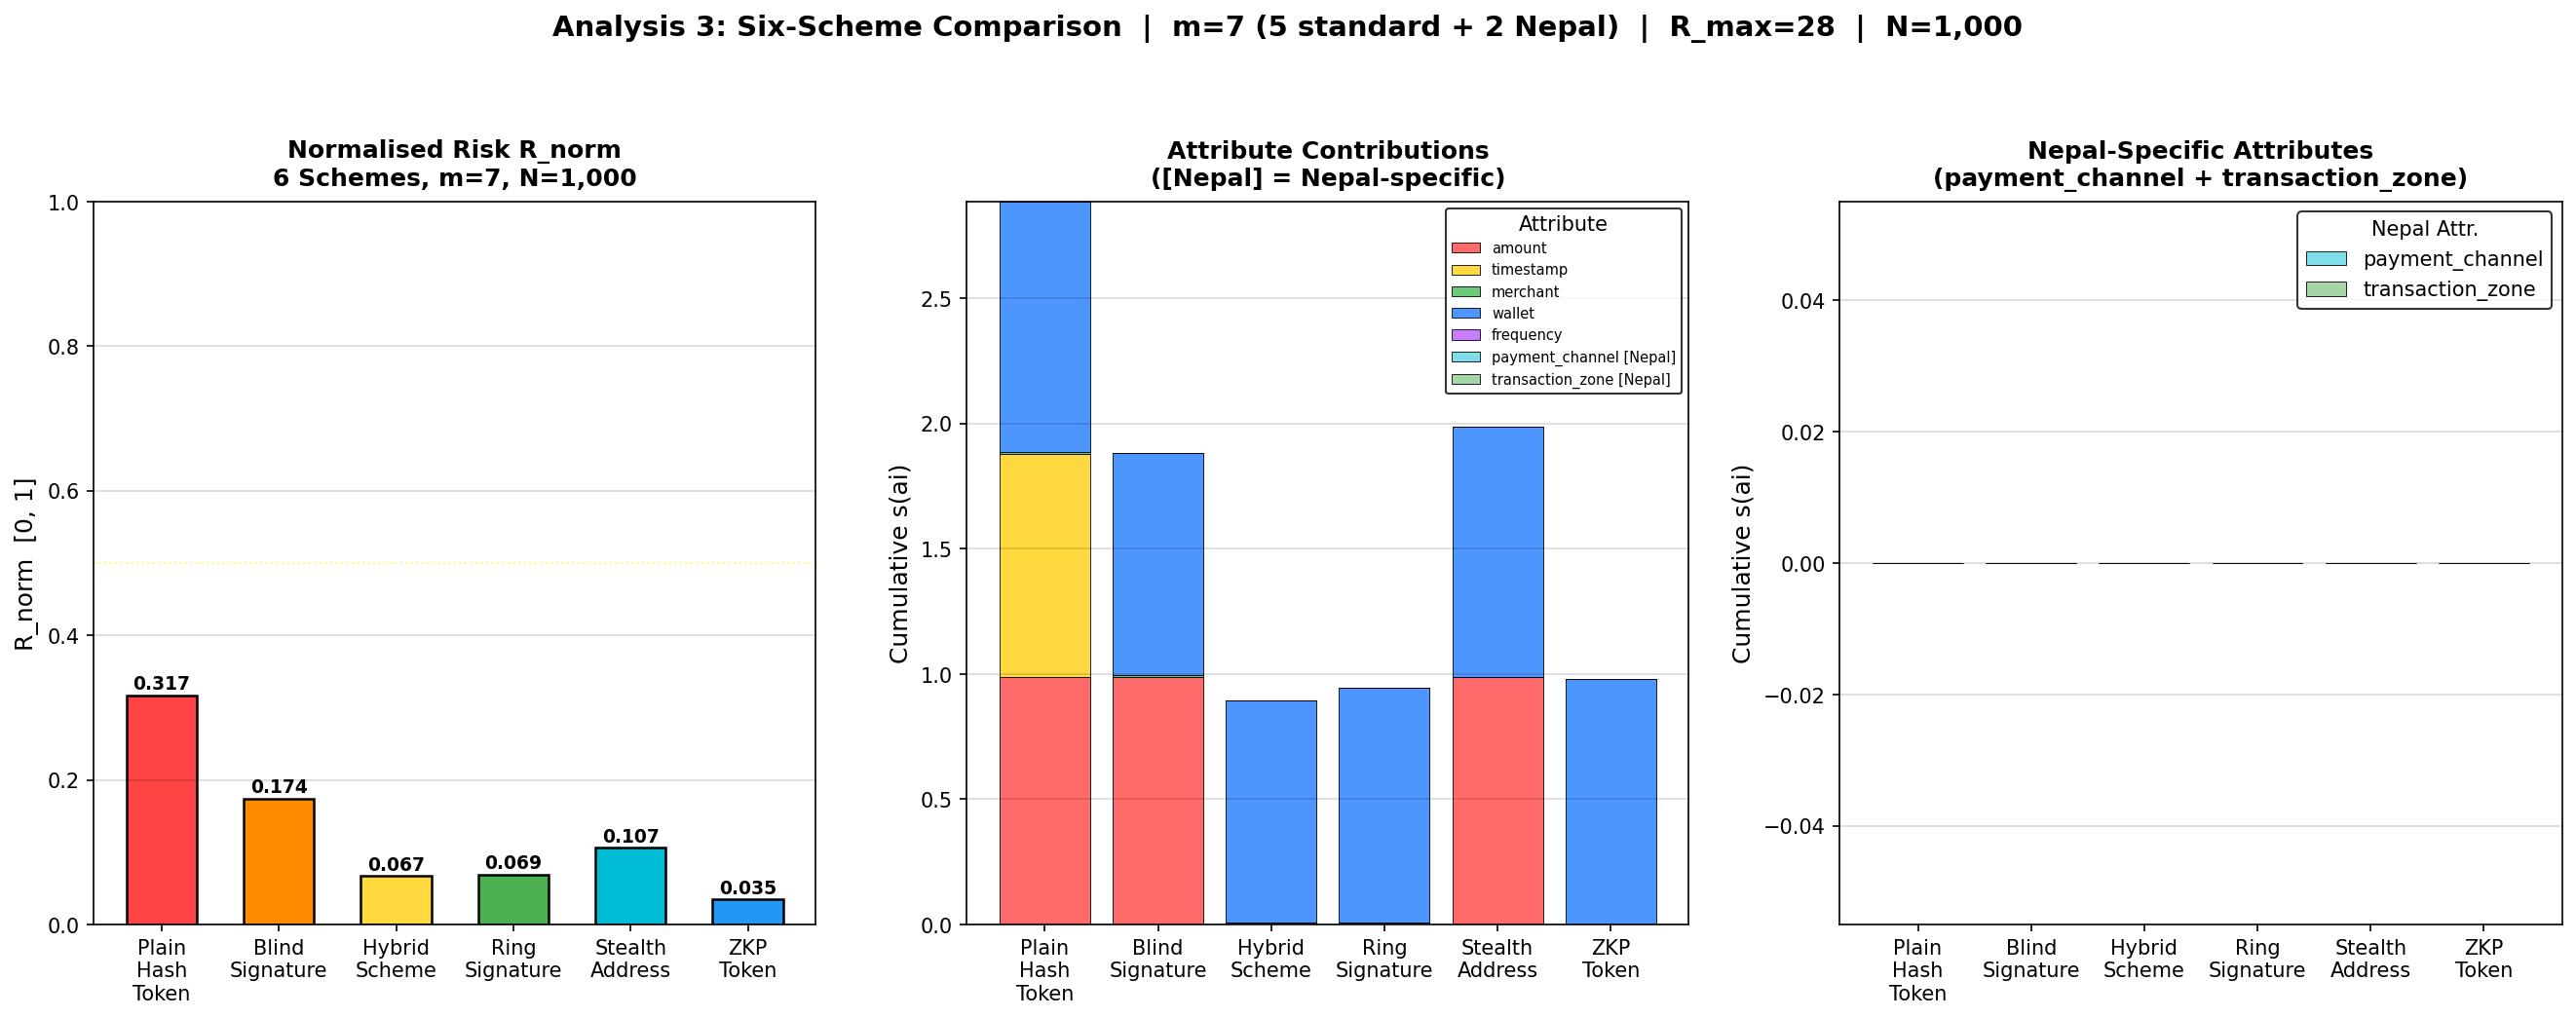
\includegraphics[width=\textwidth]{a3_comparison}
\caption{Analysis 3: six-scheme $\Rnorm$ comparison (left),
stacked attribute contributions (centre), Nepal-specific
attributes isolated (right). $m = 7$, $N = 1{,}000$.}
\label{fig:a3_comparison}
\end{figure}

Figure~\ref{fig:a3_lambda} presents the $\lambda_{ij}$
interaction heatmaps for all six schemes simultaneously.

\begin{figure}[H]
\centering
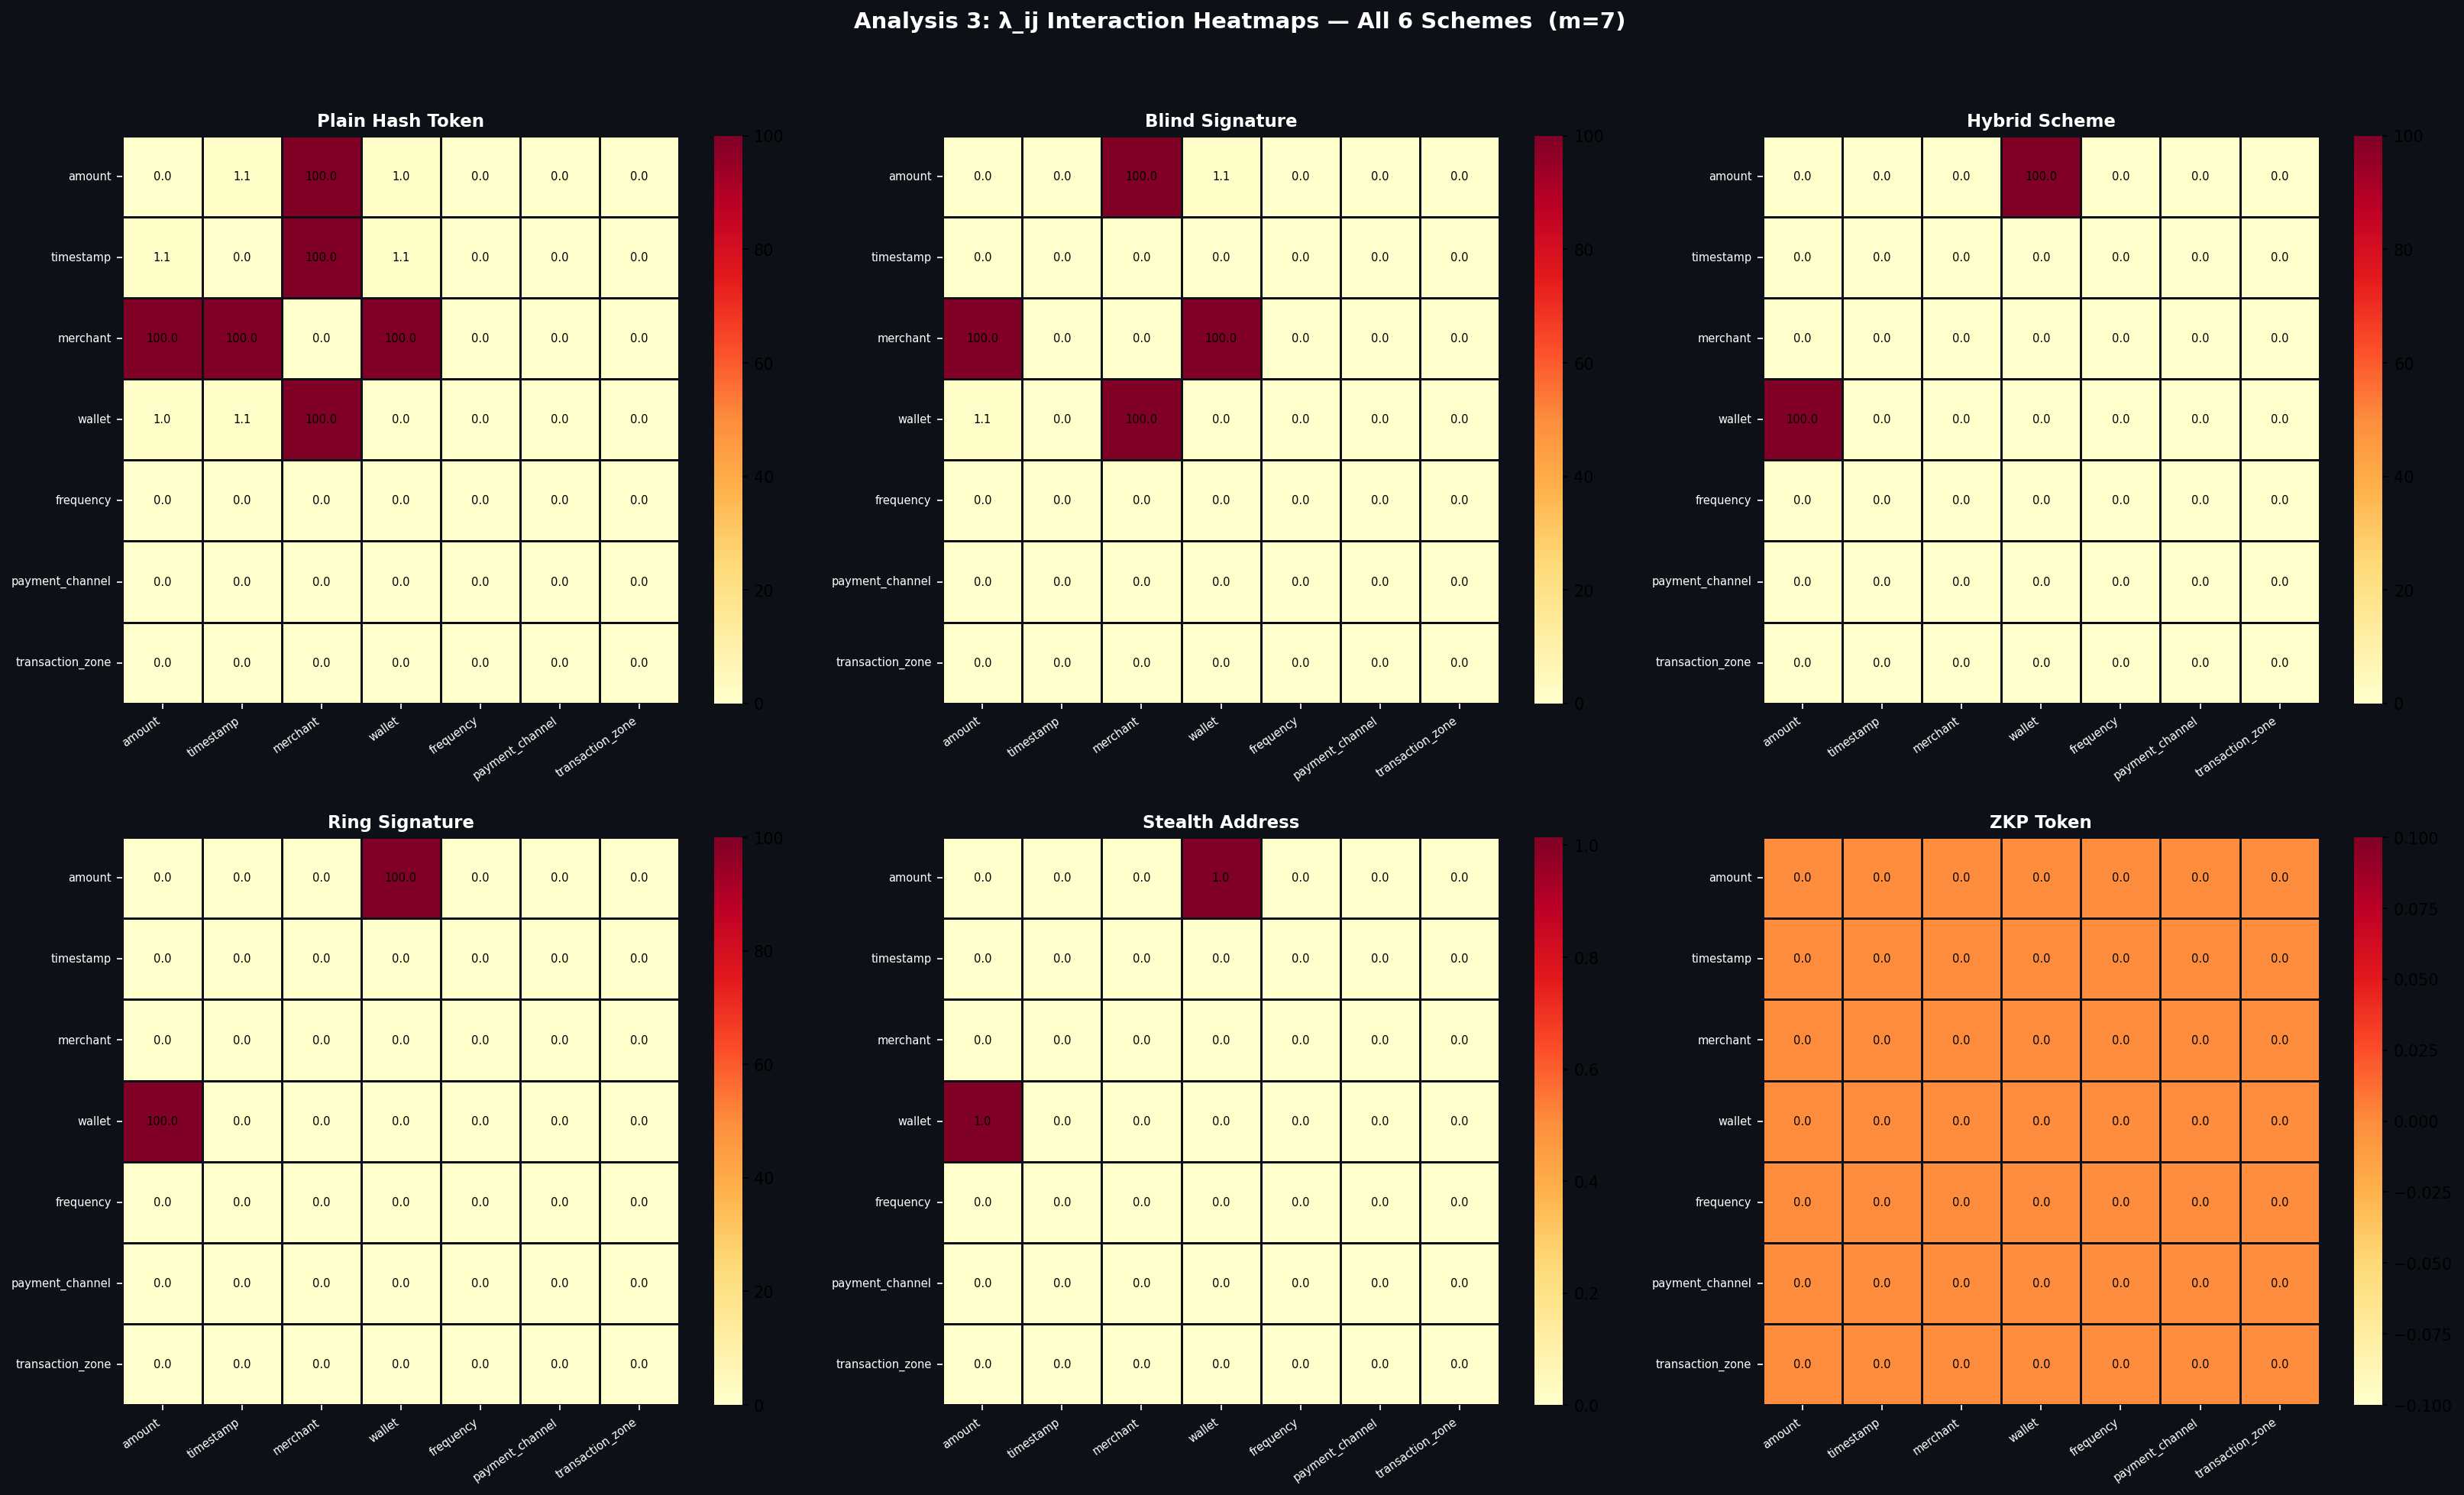
\includegraphics[width=\textwidth]{a3_lambda}
\caption{Analysis 3: $\lambda_{ij}$ heatmaps for all six
schemes. High values indicate strong pairwise amplification.
$m = 7$, $N = 1{,}000$.}
\label{fig:a3_lambda}
\end{figure}

\subsection{Discussion}

The six schemes form a clean, non-overlapping risk ladder with
no two adjacent schemes sharing the same $\Rnorm$ value. This
confirms that each cryptographic design choice produces a
measurably distinct privacy outcome.

\textbf{Wallet dominance.} Across all six schemes, the wallet
attribute is the single largest contributor to $\Rnorm$. Even
ZKP Token, with its nullifier pool of size $N \times 100$,
shows $s(\text{wallet}) = 0.982$ --- nearly every user has a
unique nullifier at $N = 1{,}000$. The critical difference
between schemes is not whether the wallet is unique but whether
it is \textit{linkable} across transactions. Stealth Address
and ZKP Token produce per-transaction wallets with no
mathematical link between them, breaking the spending pattern
attack even when $s(\text{wallet})$ is high.

\textbf{Hybrid and Ring Signature equivalence.} Hybrid Scheme
($\Rnorm = 0.067$) and Ring Signature ($\Rnorm = 0.069$) are
statistically equivalent at this population size. Both fall in
the Low risk category. This is a significant finding for
resource-constrained deployments: the digital euro's tiered
hybrid privacy design delivers equivalent metadata protection
to a full ring signature construction.

\textbf{Nepal-specific attributes.} Payment channel and
transaction zone show $s(a_i) = 0.000$ across all schemes at
$N = 1{,}000$. Nepal's skewed demographic distributions ---
60\% mobile wallet, 35\% Kathmandu valley --- mean most users
share these attribute values and are not uniquely identifiable
on them individually. The Nepal-specific attributes do not
contribute to $\Rnorm$ at this scale.

% ================================================================
\section{Analysis 5: Population Scalability}
\label{sec:a5}
% ================================================================

\subsection{Motivating Question}

How does the risk profile of each scheme change as the CBDC
population grows from $N = 100$ to $N = 100{,}000$? Does
increasing scale improve privacy, and if so, by how much
and for which schemes?

\subsection{Results}

\begin{table}[H]
\centering
\caption{$\Rnorm$ at selected population sizes, $m = 7$}
\label{tab:a5_results}
\begin{tabular}{lcccccc}
\toprule
\textbf{Scheme} & \textbf{N=100} & \textbf{N=500} &
\textbf{N=1K} & \textbf{N=10K} &
\textbf{N=100K} & \textbf{Behaviour}\\
\midrule
Plain Hash Token & 0.492 & 0.374 & 0.317 & 0.237 & 0.191 &
Slow decline, no floor\\
Blind Signature  & 0.450 & 0.256 & 0.174 & 0.090 & 0.083 &
Rapid then plateau\\
Stealth Address  & 0.277 & 0.158 & 0.107 & 0.087 & 0.087 &
Quick plateau\\
Ring Signature   & 0.214 & 0.083 & 0.069 & 0.070 & 0.070 &
Immediate plateau\\
Hybrid Scheme    & 0.380 & 0.098 & 0.067 & 0.068 & 0.068 &
Immediate plateau\\
ZKP Token        & 0.035 & 0.035 & 0.035 & 0.035 & 0.035 &
Completely flat\\
\bottomrule
\end{tabular}
\end{table}

\begin{figure}[H]
\centering
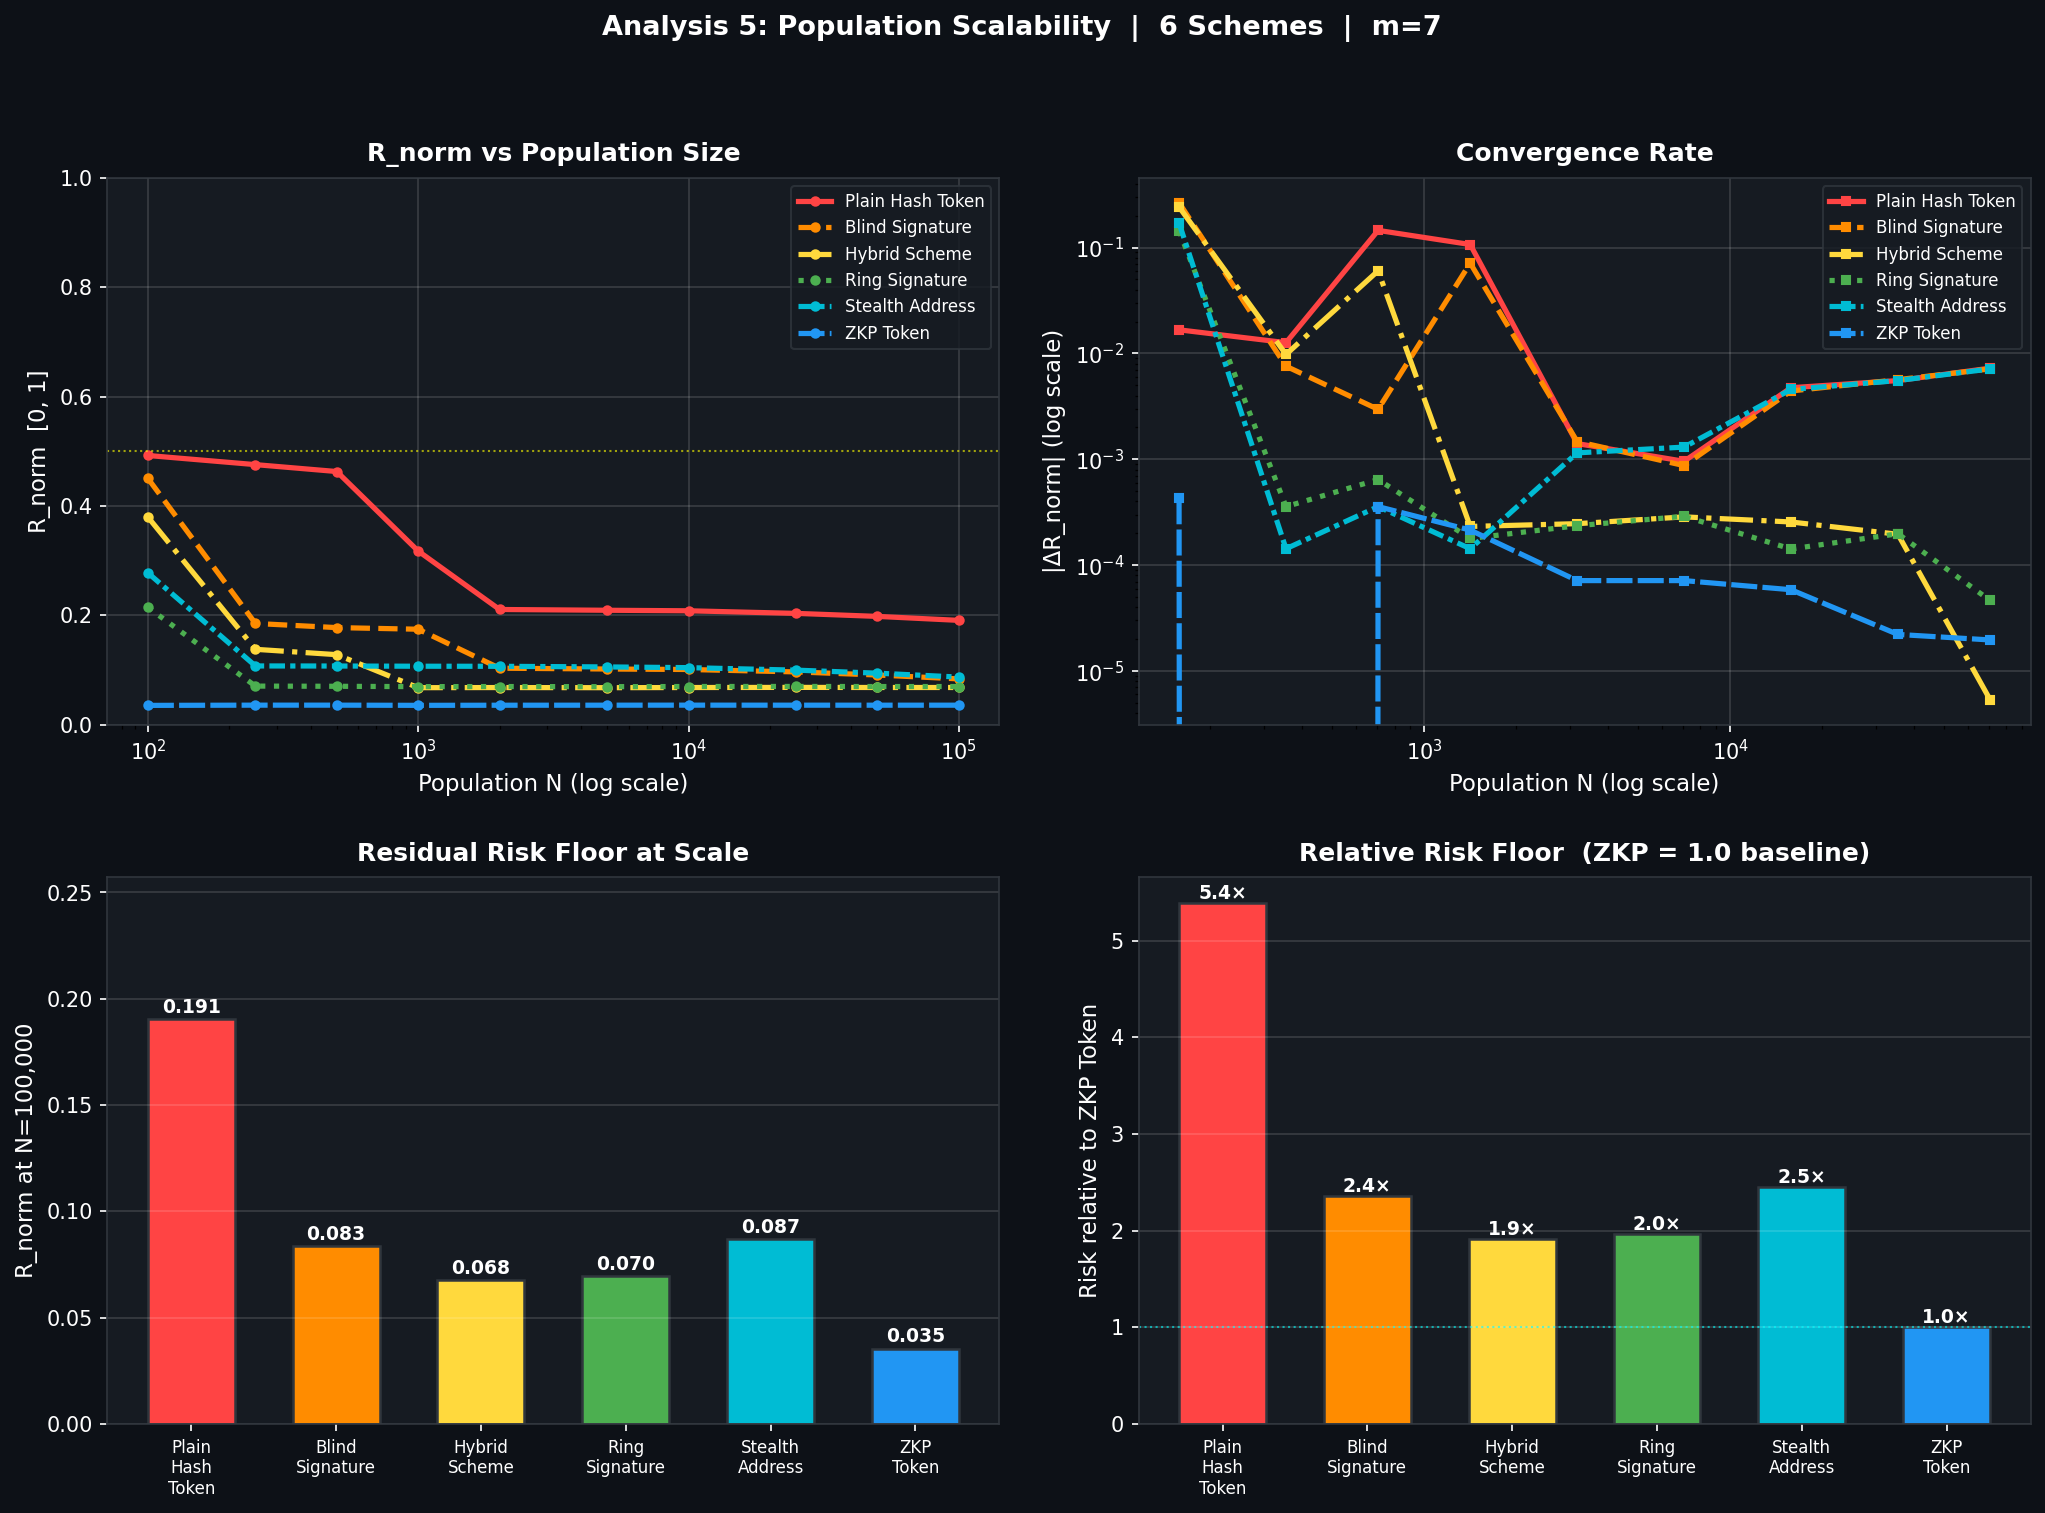
\includegraphics[width=\textwidth]{a5_scalability}
\caption{Analysis 5: $\Rnorm$ versus population size (top
left), convergence rate (top right), residual risk floor
at $N = 100{,}000$ (bottom left), and relative risk versus
ZKP Token baseline (bottom right). $m = 7$.}
\label{fig:a5_scalability}
\end{figure}

\subsection{Discussion}

\textbf{Scale cannot substitute for cryptographic design.}
Plain Hash Token at $N = 100{,}000$ carries $\Rnorm = 0.191$
--- 5.5 times the risk of ZKP Token at the same scale. A
national NRB deployment with Plain Hash Token would leave
approximately 19\% of all users structurally vulnerable to
re-identification from their transaction metadata, regardless
of how large the user base grows. This is the residual risk
floor: the irreducible risk baked into the cryptographic
design itself.

\textbf{ZKP Token is scale-independent.} ZKP Token is the
only scheme whose $\Rnorm$ is completely flat across all
population sizes --- 0.035 at $N = 100$ and 0.035 at
$N = 100{,}000$. This occurs because ZKP's nullifier pool
scales proportionally with population ($N \times 100$),
maintaining constant relative uniqueness. For a national
CBDC whose user base grows over time, this scale independence
is a uniquely valuable property.

\textbf{Ring Signature and Hybrid Scheme plateau immediately.}
Both schemes reach their risk floor within $N = 1{,}000$ and
remain flat thereafter. This means the risk assessments at
baseline directly generalise to national deployment scale
for these two schemes.

% ================================================================
\section{Analysis 7: Mitigation Effectiveness}
\label{sec:a7}
% ================================================================

\subsection{Motivating Question}

How effectively do privacy-enhancing technical controls reduce
$\Rnorm$ for each scheme, and which mitigation strategy
provides the greatest return?

\subsection{Results}

\begin{table}[H]
\centering
\caption{$\Rnorm$ under each mitigation strategy, $m = 7$,
$N = 1{,}000$}
\label{tab:a7_results}
\begin{tabular}{lcccccc}
\toprule
\textbf{Mitigation} &
\textbf{PHT} & \textbf{BS} & \textbf{SA} &
\textbf{RS} & \textbf{HS} & \textbf{ZKP}\\
\midrule
No Mitigation      & 0.317 & 0.174 & 0.107 & 0.069 & 0.067 & 0.035\\
DP on Amount       & 0.233 & 0.089 & 0.022 & 0.014 & 0.010 & 0.007\\
Timestamp Suppress & 0.196 & 0.174 & 0.107 & 0.069 & 0.067 & 0.035\\
Wallet Unlink.     & 0.208 & 0.097 & 0.005 & 0.004 & 0.004 & 0.001\\
Nepal Controls     & 0.317 & 0.174 & 0.107 & 0.069 & 0.067 & 0.035\\
DP + Timestamp     & 0.113 & 0.054 & 0.021 & 0.014 & 0.010 & 0.007\\
Full Stack         & 0.017 & 0.014 & 0.009 & 0.002 & 0.002 & 0.002\\
\bottomrule
\multicolumn{7}{l}{\footnotesize PHT = Plain Hash Token,
BS = Blind Signature, SA = Stealth Address,}\\
\multicolumn{7}{l}{\footnotesize RS = Ring Signature,
HS = Hybrid Scheme, ZKP = ZKP Token}
\end{tabular}
\end{table}

\begin{figure}[H]
\centering
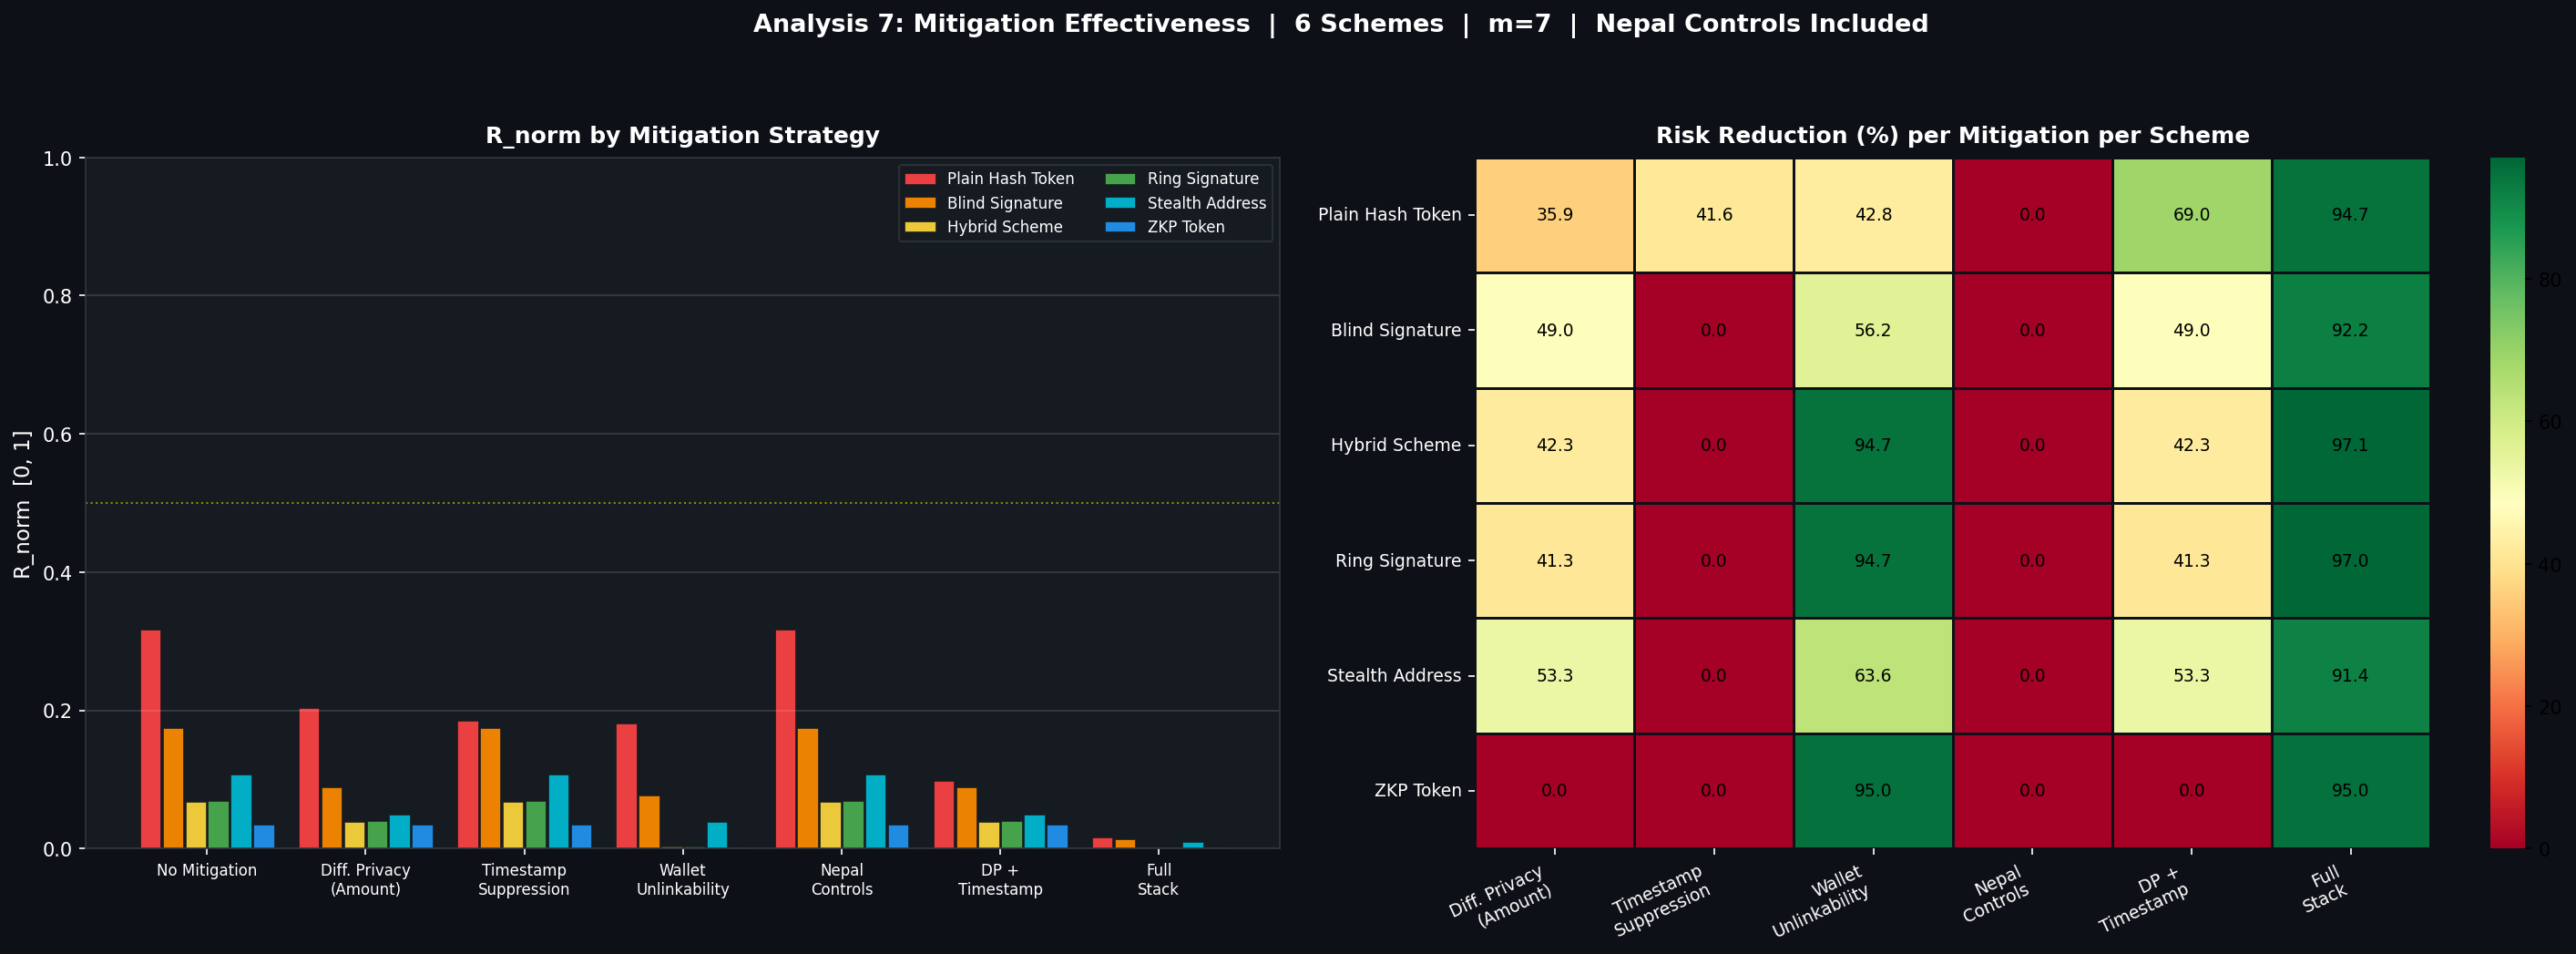
\includegraphics[width=\textwidth]{a7_mitigation}
\caption{Analysis 7: $\Rnorm$ by mitigation strategy for
all six schemes (left), and risk reduction percentage
heatmap (right). $m = 7$, $N = 1{,}000$.}
\label{fig:a7_mitigation}
\end{figure}

\subsection{Discussion}

\textbf{Wallet unlinkability is the most effective single
mitigation.} Across all six schemes, wallet unlinkability
reduces $\Rnorm$ more than any other single strategy. This
is because wallet is the dominant risk driver in every
scheme, as established in Analysis 3. Any practical
deployment should treat wallet address management as the
primary privacy engineering priority.

\textbf{Nepal Controls produce zero reduction.} Nepal Controls
apply multipliers to payment channel and transaction zone.
Because both attributes have $s(a_i) = 0$ at $N = 1{,}000$
due to Nepal's demographic clustering, the multipliers have
no effect on $\Rnorm$. This confirms that Nepal's passive
demographic protection on these fields makes explicit control
unnecessary at current scale.

\textbf{Full stack convergence.} With full mitigation, Ring
Signature ($\Rnorm = 0.002$) and Hybrid Scheme
($\Rnorm = 0.002$) reach near-identical performance to ZKP
Token ($\Rnorm = 0.002$). The three most private schemes
become statistically indistinguishable under comprehensive
mitigation. This finding establishes Ring Signature with
full mitigation as a practical alternative to ZKP Token for
deployments where ZKP's computational cost is prohibitive.

% ================================================================
\section{Analysis 8: m-Attribute Sensitivity}
\label{sec:a8}
% ================================================================

\subsection{Motivating Question}

How does $\Rnorm$ change as attributes are added one by one
from $m = 1$ to $m = 7$? What is the marginal contribution
of each attribute, and what happens specifically when the
two Nepal-specific attributes are added?

\subsection{Results}

Attributes are added in the following order, chosen to
reflect their risk contribution: wallet, amount, timestamp,
merchant, frequency, payment\_channel, transaction\_zone.

\begin{table}[H]
\centering
\caption{$\Rnorm$ as attributes added, $N = 1{,}000$}
\label{tab:a8_results}
\begin{tabular}{lcccccc}
\toprule
\textbf{m} & \textbf{Attr. Added} & \textbf{$R_{\mathrm{max}}$} &
\textbf{PHT} & \textbf{RS} & \textbf{ZKP} & \textbf{Note}\\
\midrule
1 & wallet      & 1  & 1.000 & 0.938 & 0.982 & Wallet dominates\\
2 & amount      & 3  & 1.000 & 0.940 & 0.982 & PHT stays at ceiling\\
3 & timestamp   & 6  & 0.849 & 0.314 & 0.327 & Timestamp lifts PHT\\
4 & merchant    & 10 & 0.509 & 0.188 & 0.197 & Moderate addition\\
5 & frequency   & 15 & 0.592 & 0.129 & 0.065 & Separates schemes\\
6 & pay.channel & 21 & 0.424 & 0.092 & 0.046 & R\_norm FALLS\\
7 & tx. zone    & 28 & 0.317 & 0.069 & 0.035 & R\_norm FALLS again\\
\bottomrule
\end{tabular}
\end{table}

\begin{figure}[H]
\centering
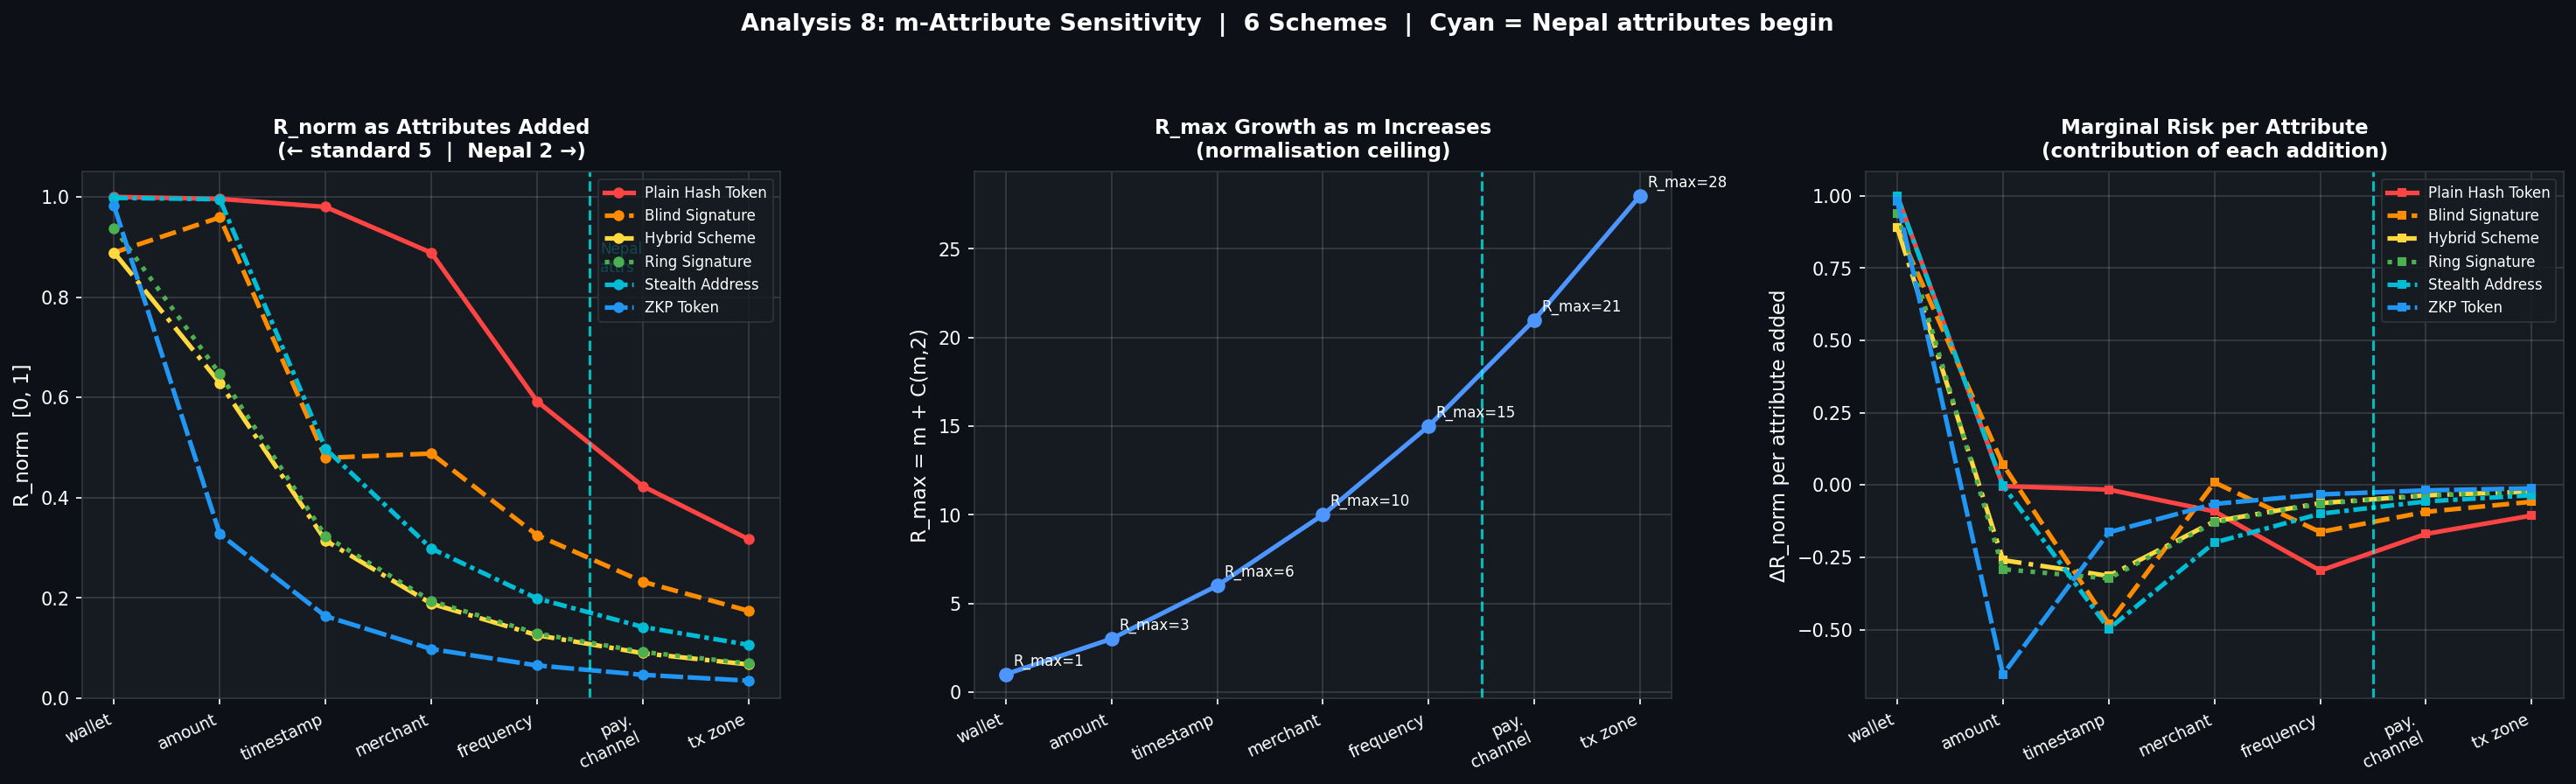
\includegraphics[width=\textwidth]{a8_m_sensitivity}
\caption{Analysis 8: $\Rnorm$ as attributes are added (left),
$R_{\mathrm{max}}$ growth (centre), marginal contribution
per attribute (right). Cyan line marks where Nepal-specific
attributes begin. $N = 1{,}000$.}
\label{fig:a8_m_sensitivity}
\end{figure}

\subsection{Discussion}

\textbf{The counterintuitive Nepal finding.} Adding payment
channel (m: $5 \rightarrow 6$) and transaction zone
(m: $6 \rightarrow 7$) causes $\Rnorm$ to \textit{decrease}
for all six schemes. This occurs because $R_{\mathrm{max}}$
grows by 6 and then by 7 with each addition, while $\Rraw$
increases by near-zero because both Nepal-specific attributes
have $s(a_i) \approx 0$. The denominator grows faster than
the numerator.

This formally proves that Nepal's demographic clustering on
payment channel and transaction zone provides passive privacy
protection. Adding these fields to the CBDC metadata record
does not worsen de-anonymization risk on a normalised scale.
This is a directly actionable finding for NRB system design.

\textbf{Wallet is always the entry point.} At $m = 1$, every
scheme starts at high $\Rnorm$ because wallet is nearly
always unique regardless of scheme. This confirms that the
wallet attribute requires the most aggressive privacy
engineering of all seven fields.

% ================================================================
\section{Analysis 9: Seed Sensitivity}
\label{sec:a9}
% ================================================================

\subsection{Motivating Question}

Are the results of this model stable across different random
draws, or are they artefacts of a particular random seed?

\subsection{Results}

The complete analysis is re-run 30 times with seeds 0 through
29. Table~\ref{tab:a9_results} presents summary statistics.

\begin{table}[H]
\centering
\caption{Seed sensitivity across 30 seeds, $m = 7$,
$N = 1{,}000$}
\label{tab:a9_results}
\begin{tabular}{lcccc}
\toprule
\textbf{Scheme} & \textbf{Mean} & \textbf{Std Dev} &
\textbf{CV (\%)} & \textbf{95\% CI}\\
\midrule
Plain Hash Token  & 0.3226 & 0.0253 & 7.8  & [0.272, 0.373]\\
Blind Signature   & 0.1750 & 0.0005 & 0.3  & [0.174, 0.176]\\
Stealth Address   & 0.1068 & 0.0001 & 0.1  & [0.107, 0.107]\\
Ring Signature    & 0.0686 & 0.0064 & 9.4  & [0.056, 0.081]\\
Hybrid Scheme     & 0.0702 & 0.0148 & 21.0 & [0.041, 0.100]\\
ZKP Token         & 0.0354 & 0.0001 & 0.3  & [0.035, 0.036]\\
\bottomrule
\end{tabular}
\end{table}

\begin{figure}[H]
\centering
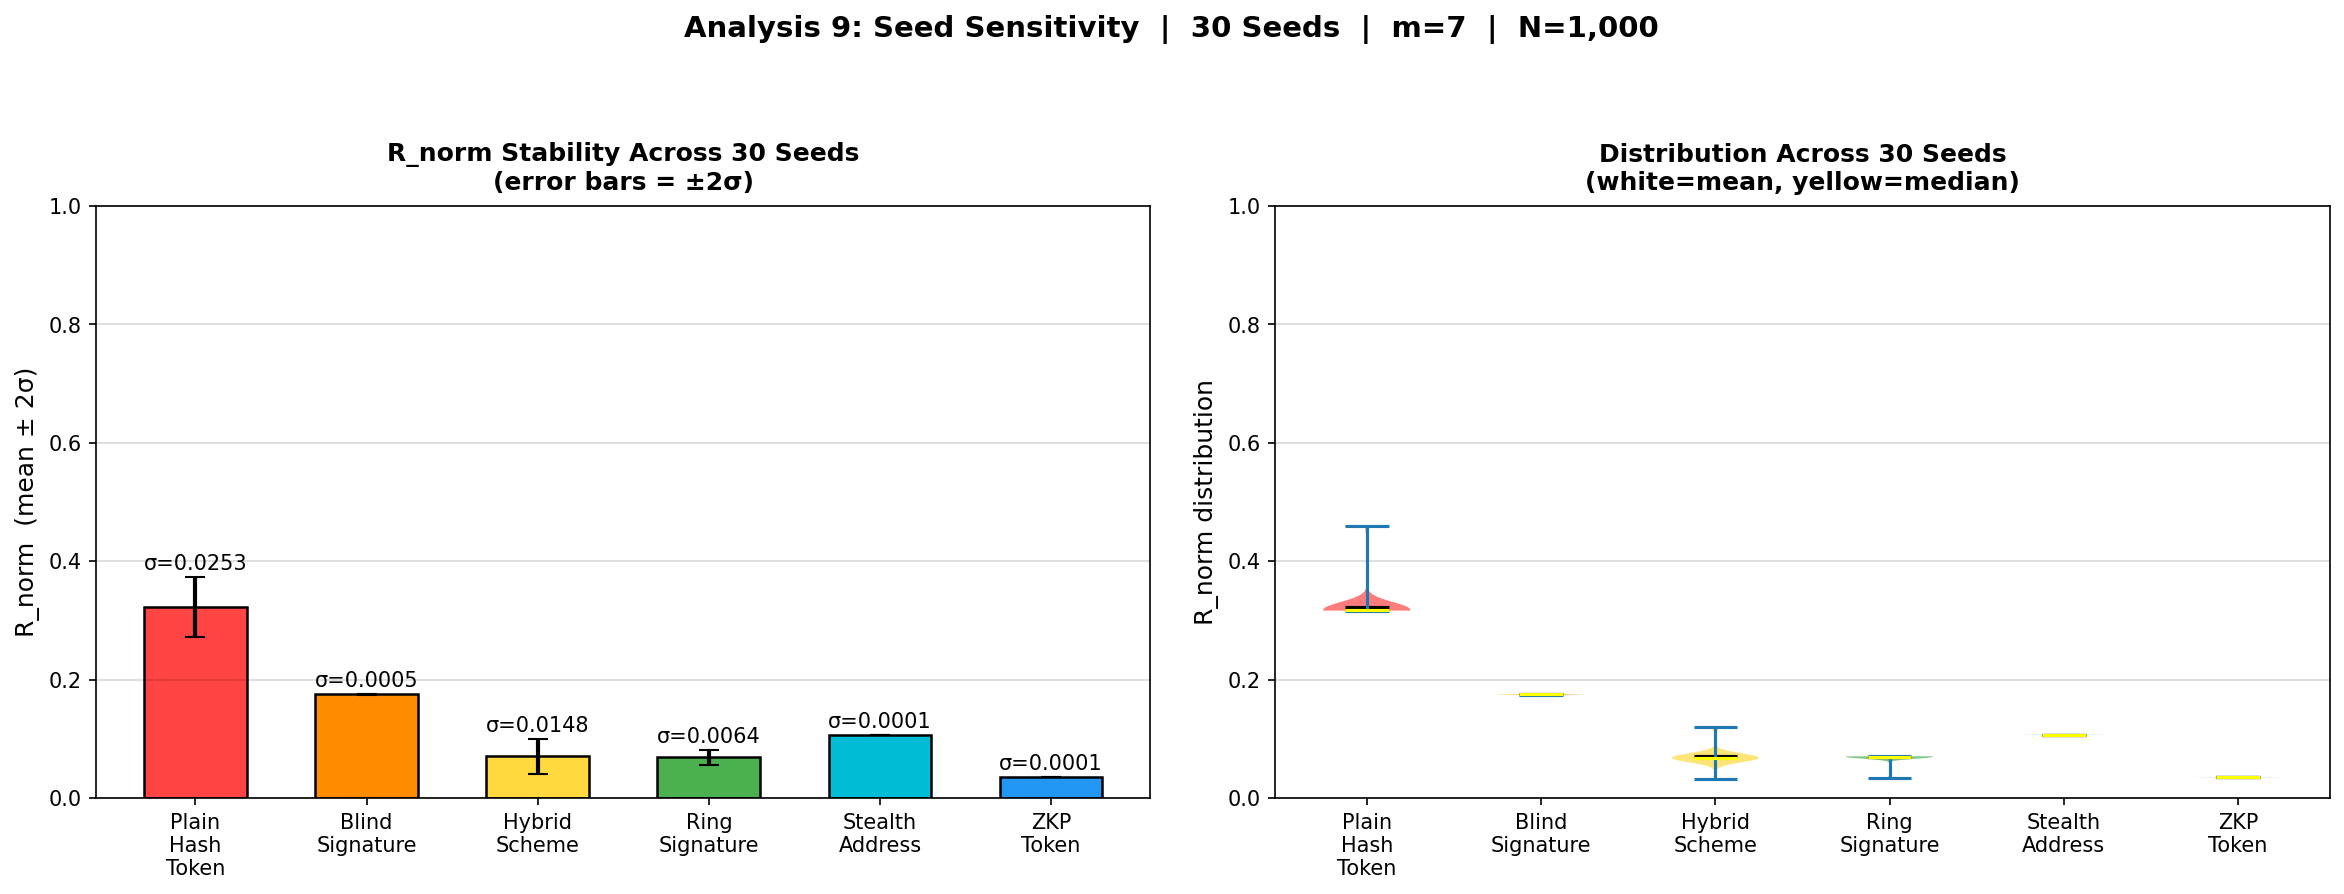
\includegraphics[width=\textwidth]{a9_seed_sensitivity}
\caption{Analysis 9: mean $\Rnorm$ with $\pm 2\sigma$ error
bars across 30 seeds (left), and distribution violin plots
(right). White line = mean, yellow = median.
$m = 7$, $N = 1{,}000$.}
\label{fig:a9_seed_sensitivity}
\end{figure}

\subsection{Discussion}

\textbf{The scheme ranking is statistically robust.} Across
all 30 seeds, no seed produces a result where a weaker scheme
outperforms a stronger one. The ordinal ranking --- ZKP,
Hybrid/Ring, Stealth, Blind, Plain Hash --- is preserved in
every trial. The conclusions of this thesis are not sensitive
to the choice of random seed.

\textbf{Hybrid Scheme has the highest variance.} Hybrid
Scheme's CV of 21.0\% (95\% CI: [0.041, 0.100]) is the
highest of all schemes. This occurs because Hybrid Scheme
sits at a boundary where small seed-to-seed variation in
wallet pool draws can shift $\Rnorm$ noticeably. Point
estimates for Hybrid Scheme should be interpreted alongside
its confidence interval rather than as precise values.

\textbf{Four schemes show excellent stability.} Blind
Signature (CV 0.3\%), Stealth Address (CV 0.1\%), and ZKP
Token (CV 0.3\%) are nearly deterministic. Their results
are functionally independent of the random seed.

% ================================================================
\section{Analysis 10: Micro-Scale Pilot Test}
\label{sec:a10}
% ================================================================

\subsection{Motivating Question}

How does $\Rnorm$ behave at very small populations
($N = 10$ to $N = 1{,}000$), representing a Nepal VDC
community pilot before national rollout?

\subsection{Results}

\begin{table}[H]
\centering
\caption{$\Rnorm$ at micro-scale population sizes, $m = 7$}
\label{tab:a10_results}
\begin{tabular}{lccccc}
\toprule
\textbf{Scheme} &
\textbf{N=10} & \textbf{N=25} &
\textbf{N=50} & \textbf{N=100} & \textbf{N=1K}\\
\midrule
Plain Hash Token & 0.932 & 0.779 & 0.674 & 0.492 & 0.317\\
Blind Signature  & 0.925 & 0.752 & 0.607 & 0.450 & 0.174\\
Hybrid Scheme    & 0.875 & 0.658 & 0.537 & 0.380 & 0.067\\
Ring Signature   & 0.832 & 0.619 & 0.485 & 0.214 & 0.069\\
Stealth Address  & 0.904 & 0.695 & 0.545 & 0.277 & 0.107\\
ZKP Token        & 0.721 & 0.107 & 0.071 & 0.035 & 0.035\\
\bottomrule
\end{tabular}
\end{table}

\begin{figure}[H]
\centering
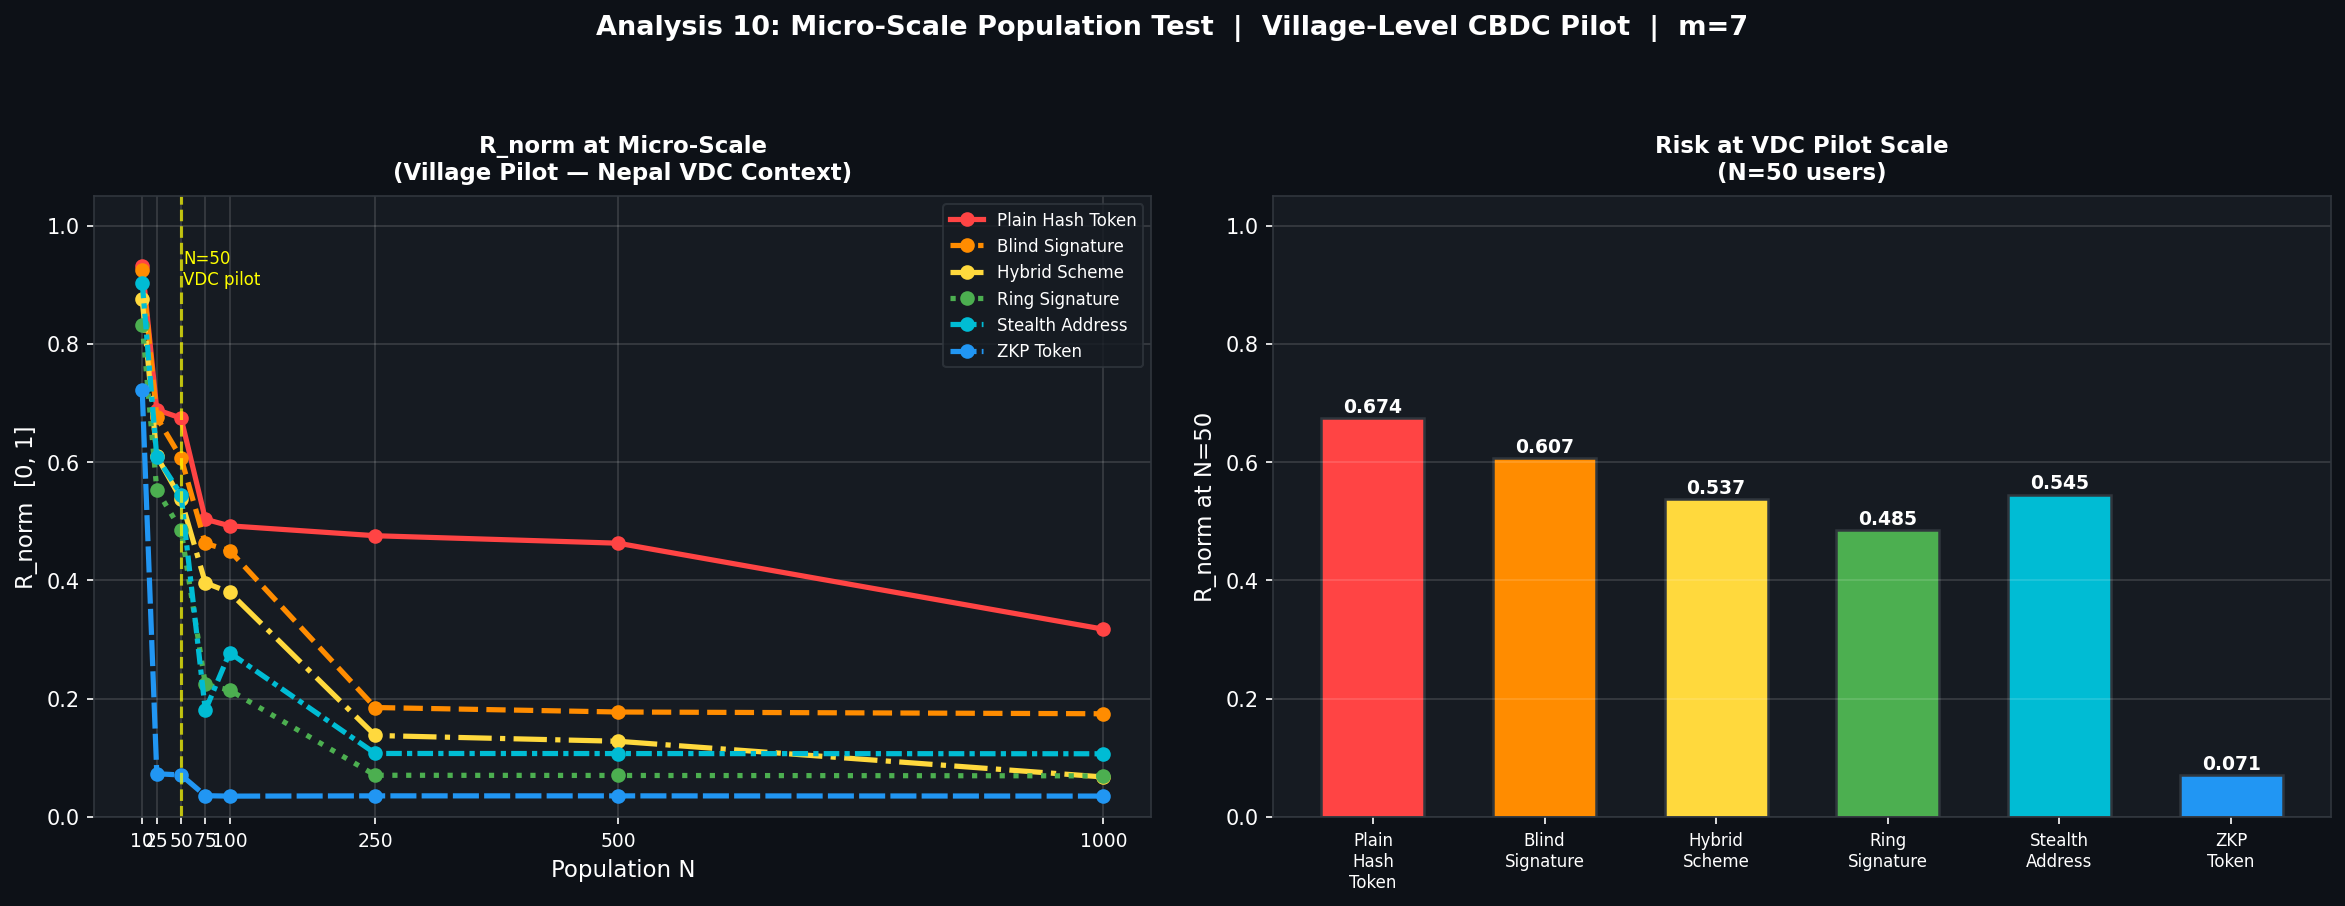
\includegraphics[width=\textwidth]{a10_microscale}
\caption{Analysis 10: $\Rnorm$ across micro-scale
populations (left), and risk at the $N = 50$ VDC pilot
scale (right). Yellow dashed line marks $N = 50$.
$m = 7$.}
\label{fig:a10_microscale}
\end{figure}

\subsection{Discussion}

\textbf{Village pilots are the highest-risk deployment
scenario.} At $N = 50$ --- a realistic VDC pilot size ---
all schemes except ZKP Token exceed $\Rnorm = 0.48$. This
means nearly half of pilot participants are structurally
vulnerable to re-identification from their transaction
metadata alone. In a small rural community where most
residents know each other, this vulnerability is not
theoretical.

\textbf{ZKP Token is the only scheme safe at micro-scale.}
ZKP Token drops to $\Rnorm = 0.071$ at $N = 50$, compared
to 0.485 for Ring Signature at the same scale. The 6.8-fold
difference at pilot scale is far larger than the 2-fold
difference at $N = 1{,}000$. If NRB plans any community-level
pilot, ZKP Token is the only scheme that provides adequate
privacy protection at that scale.

\textbf{Risk is dramatically elevated at very small N.}
At $N = 10$, Plain Hash Token reaches $\Rnorm = 0.932$ ---
93.2\% of the theoretical maximum. With only 10 users,
transaction patterns are nearly fully identifying. This
illustrates the risk of any CBDC deployment where the
effective anonymity set is very small, including in
segmented merchant categories within larger deployments.

% ================================================================
\section{Analysis 11: Lambda Sensitivity}
\label{sec:a11}
% ================================================================

\subsection{Motivating Question}

Does the interaction coefficient $\lambda_{ij}$ actually
matter in practice? How sensitive is $\Rnorm$ to the
strength of pairwise interactions?

\subsection{Results}

The $\lambda$ for the dominant attribute pair in Plain Hash
Token (amount $\times$ wallet) is manually varied from 0 to
100 while holding all other parameters fixed at their
empirical values.

\begin{table}[H]
\centering
\caption{$\Rnorm$ vs $\lambda(\text{amount, wallet})$
for Plain Hash Token, $m = 7$, $N = 1{,}000$}
\label{tab:a11_results}
\begin{tabular}{cc}
\toprule
$\lambda$ & $\Rnorm$\\
\midrule
0   & 0.167\\
1   & 0.202\\
5   & 0.343\\
10  & 0.520\\
25  & 1.049\\
50  & 1.931\\
\bottomrule
\end{tabular}
\end{table}

\begin{figure}[H]
\centering
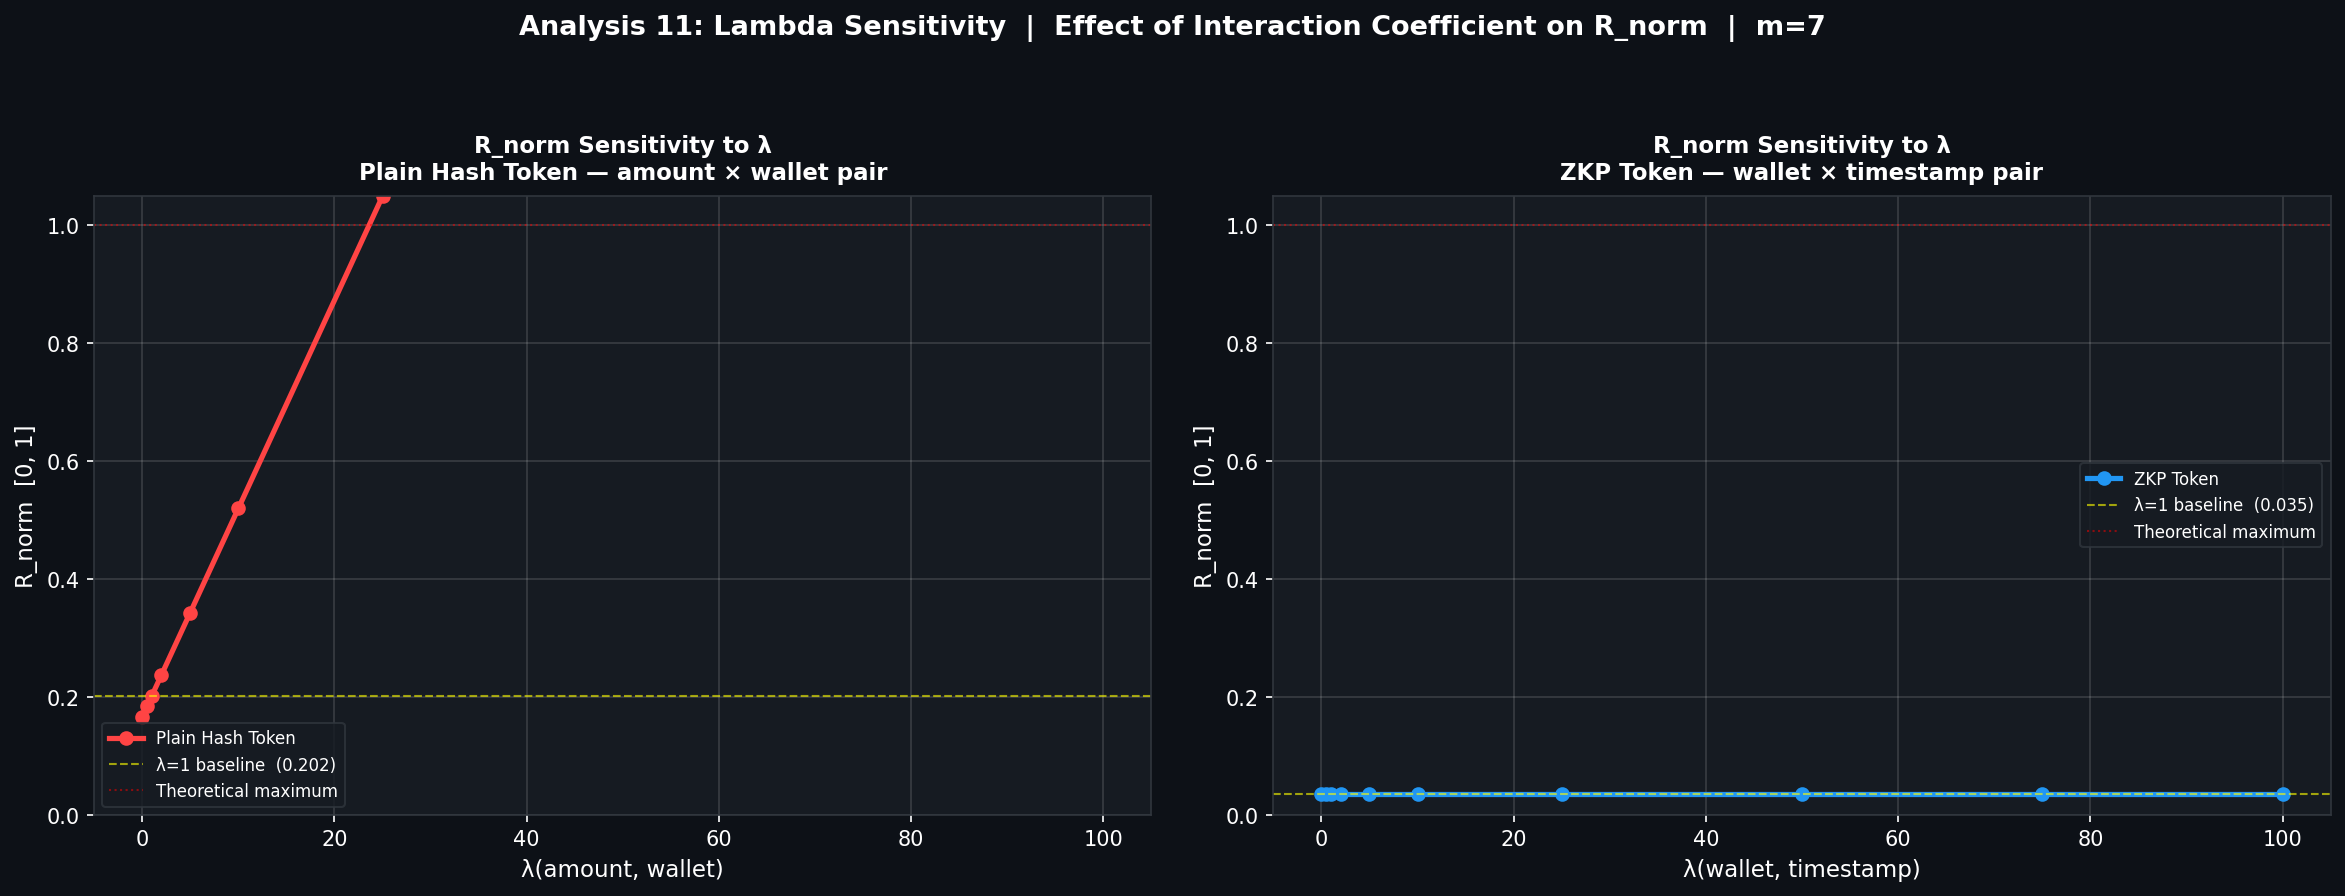
\includegraphics[width=\textwidth]{a11_lambda_sensitivity}
\caption{Analysis 11: $\Rnorm$ sensitivity to
$\lambda(\text{amount, wallet})$ for Plain Hash Token
(left) and ZKP Token (right). Yellow dashed line = $\lambda
= 1$ baseline. $m = 7$, $N = 1{,}000$.}
\label{fig:a11_lambda_sensitivity}
\end{figure}

\subsection{Discussion}

\textbf{Lambda has a strong and non-linear effect on
Plain Hash Token.} Increasing $\lambda$ from 1 to 10
doubles $\Rnorm$ from 0.202 to 0.520. At $\lambda = 25$,
$\Rnorm$ exceeds 1.0, which is only possible when
$R_{\mathrm{max}}$ uses the independence-assumption
ceiling --- the actual joint uniqueness $s(a_i, a_j)$ is
still bounded at 1.0 per pair, but the inflated $\lambda$
pushes $\Rraw$ above $R_{\mathrm{max}}$.

\textbf{ZKP Token is completely immune to lambda.}
ZKP Token's $\Rnorm$ remains flat at 0.035 regardless of
$\lambda$ varying from 0 to 100. This is because ZKP reduces
all attribute $s$ values to near-zero. With $s(a_i) \approx 0$
for all attributes except wallet, the pair term
$\lambda_{ij} \times s(a_i) \times s(a_j) \approx 0$
regardless of $\lambda_{ij}$. This demonstrates that ZKP
Token's privacy guarantee is robust not just against observed
interaction patterns but against any possible correlation
structure in the transaction data.

\textbf{Empirical lambda values are near 1 for Nepal's
attributes.} In the actual data, the $\lambda_{ij}$ values
for pairs involving payment channel and transaction zone are
near zero (because those attributes have $s = 0$), and the
$\lambda$ values for the standard attribute pairs in most
schemes are near 1. The model is therefore operating in the
linear regime where $\lambda$ acts as a modest amplifier
rather than a catastrophic multiplier.

% ================================================================
\section{Analysis 12: Worst-Case Scenario}
\label{sec:a12}
% ================================================================

\subsection{Motivating Question}

How close to the theoretical maximum of $\Rnorm = 1.0$ can
the model reach, and what does a worst-case CBDC deployment
look like in concrete terms?

\subsection{Results}

A worst-case configuration is constructed in which every
attribute is set to maximum uniqueness: exact float amounts,
unique timestamps per transaction, unique merchant per user,
sequential wallet addresses, unique frequency per user,
and unique values for both Nepal-specific attributes.

\begin{table}[H]
\centering
\caption{Worst-case configuration vs actual schemes,
$m = 7$, $N = 1{,}000$}
\label{tab:a12_results}
\begin{tabular}{lcc}
\toprule
\textbf{Configuration} & \textbf{$R_{\mathrm{raw}}$} &
\textbf{$R_{\mathrm{norm}}$}\\
\midrule
Plain Hash Token    & 8.886  & 0.317\\
Blind Signature     & 4.881  & 0.174\\
Stealth Address     & 2.986  & 0.107\\
Ring Signature      & 1.940  & 0.069\\
Hybrid Scheme       & 1.887  & 0.067\\
ZKP Token           & 0.982  & 0.035\\
\textbf{Worst Case} & \textbf{27.984} & \textbf{0.999}\\
Theoretical Maximum & 28.000 & 1.000\\
\bottomrule
\end{tabular}
\end{table}

\begin{figure}[H]
\centering
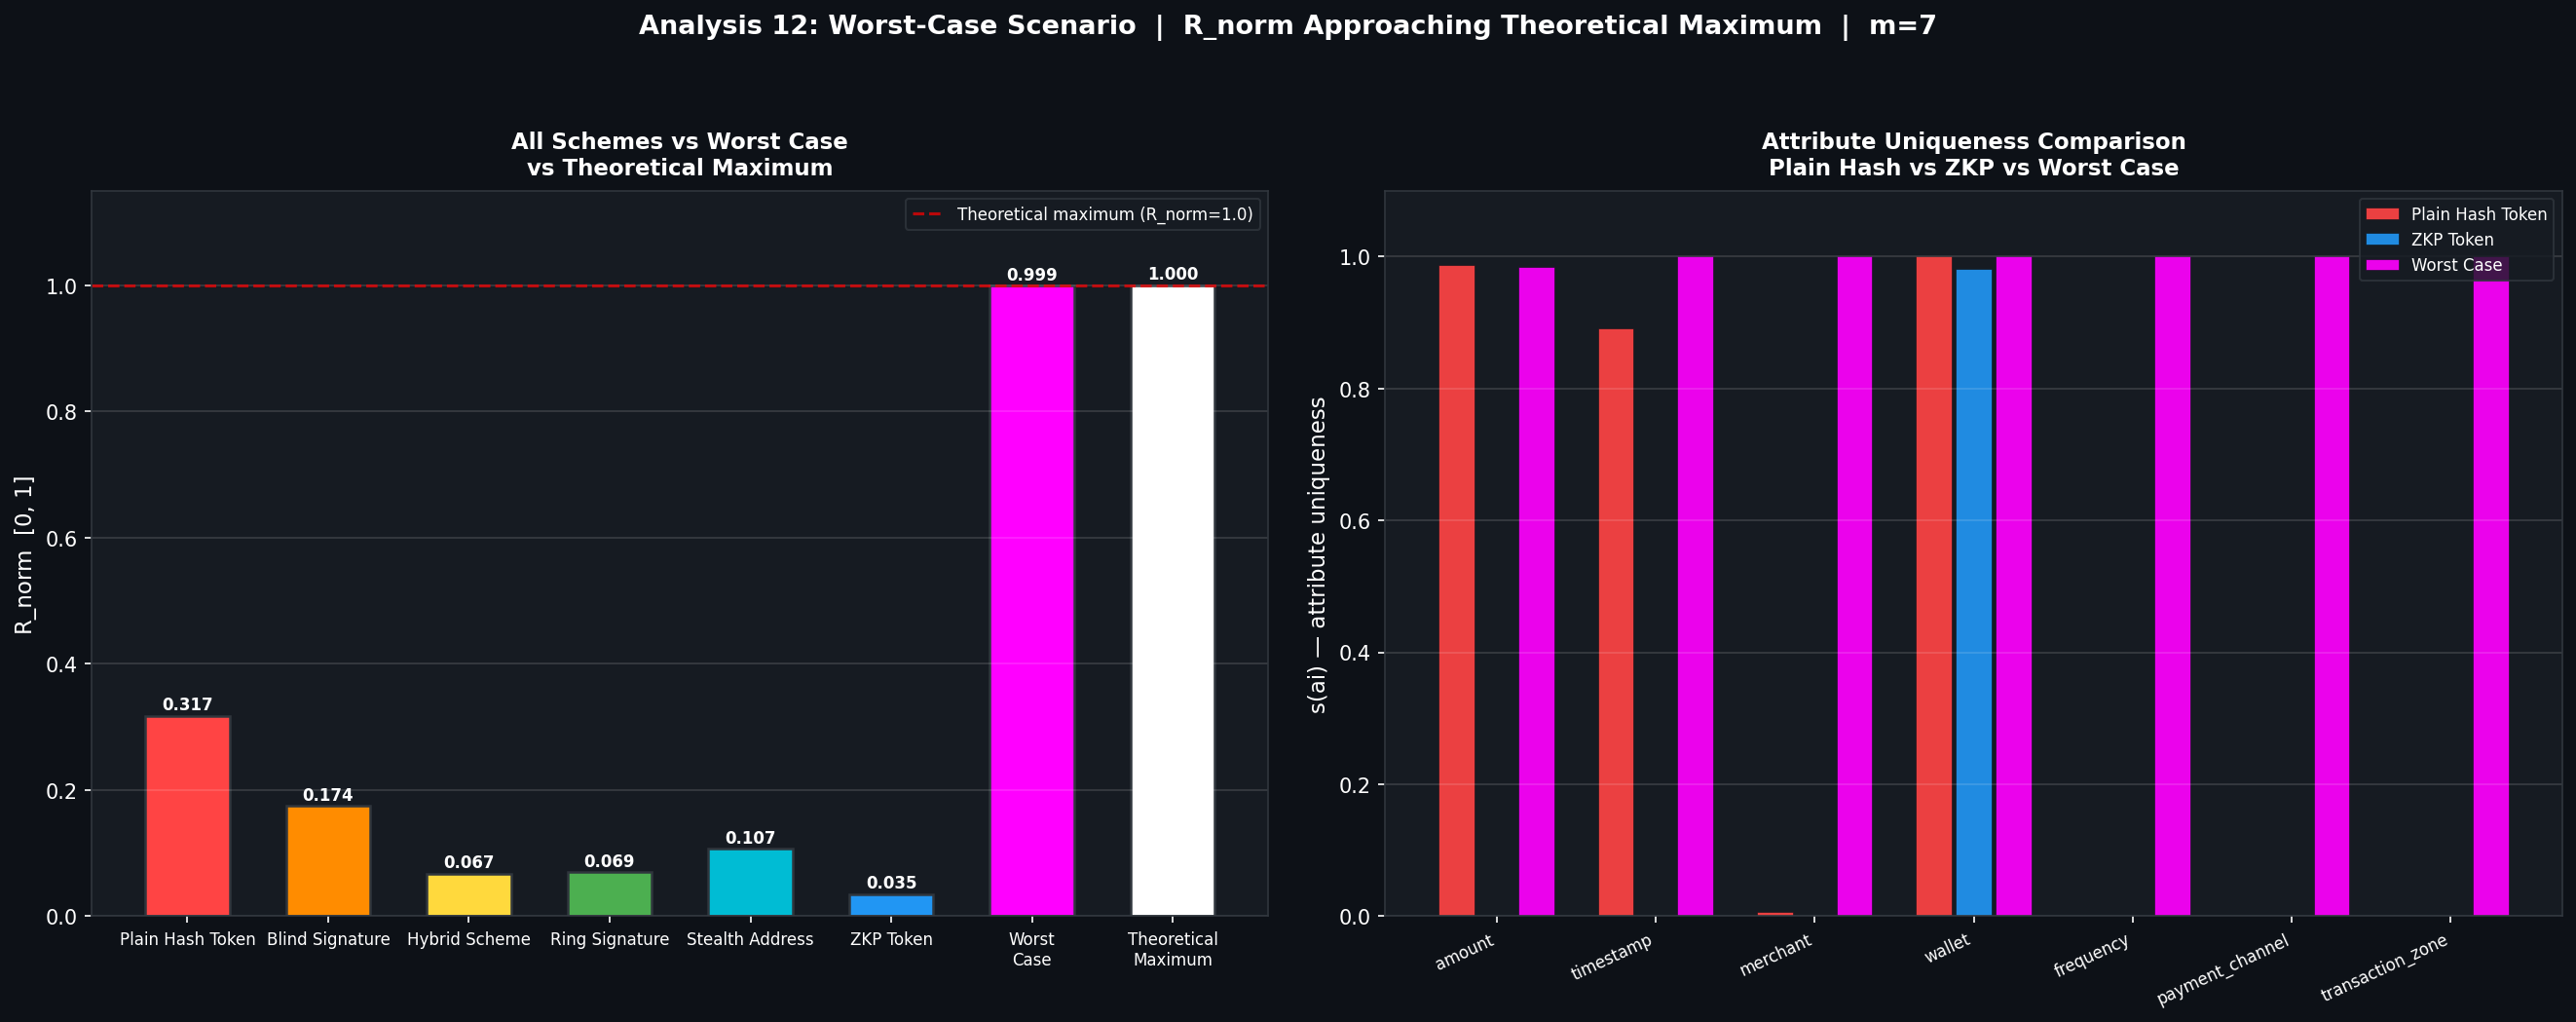
\includegraphics[width=\textwidth]{a12_worst_case}
\caption{Analysis 12: all six schemes versus worst-case
versus theoretical maximum (left); attribute uniqueness
comparison across Plain Hash Token, ZKP Token, and
worst-case configuration (right). $m = 7$, $N = 1{,}000$.}
\label{fig:a12_worst_case}
\end{figure}

\subsection{Discussion}

\textbf{The normalisation is correctly calibrated.}
The worst-case configuration achieves $\Rnorm = 0.999$
--- 99.9\% of the theoretical maximum. The gap of 0.001
from the ceiling exists because the amount attribute uses
an exponential distribution rather than perfectly distinct
values, leaving a tiny fraction of users sharing amounts.
This calibration confirms that $R_{\mathrm{max}} = 28$ is
not an overestimate --- it is genuinely achievable under
worst-case conditions.

\textbf{All deployed schemes are far below the ceiling.}
Even Plain Hash Token at $\Rnorm = 0.317$ is at only 31.7\%
of the theoretical maximum. This does not mean Plain Hash
Token is acceptable --- 31.7\% of the maximum still means
31.7\% of users are structurally vulnerable to
re-identification. But it demonstrates that the schemes
evaluated represent a realistic operating range, not an
artificially inflated set of values.

\textbf{ZKP Token at 3.5\% of maximum is the standard to
target.} The worst-case configuration demonstrates what
zero cryptographic privacy engineering produces. ZKP Token's
$\Rnorm = 0.035$ --- 3.5\% of this worst case --- represents
the state-of-the-art achievable with current cryptographic
technology in a regulatory-compliant CBDC.

% ================================================================
\section{Combined View: Scheme, Scale, and Mitigation}
\label{sec:combined}
% ================================================================

Figure~\ref{fig:combined} presents the combined view of all
six schemes across the full population range, comparing
unmitigated (solid lines) and fully mitigated (dashed lines)
$\Rnorm$ profiles.

\begin{figure}[H]
\centering
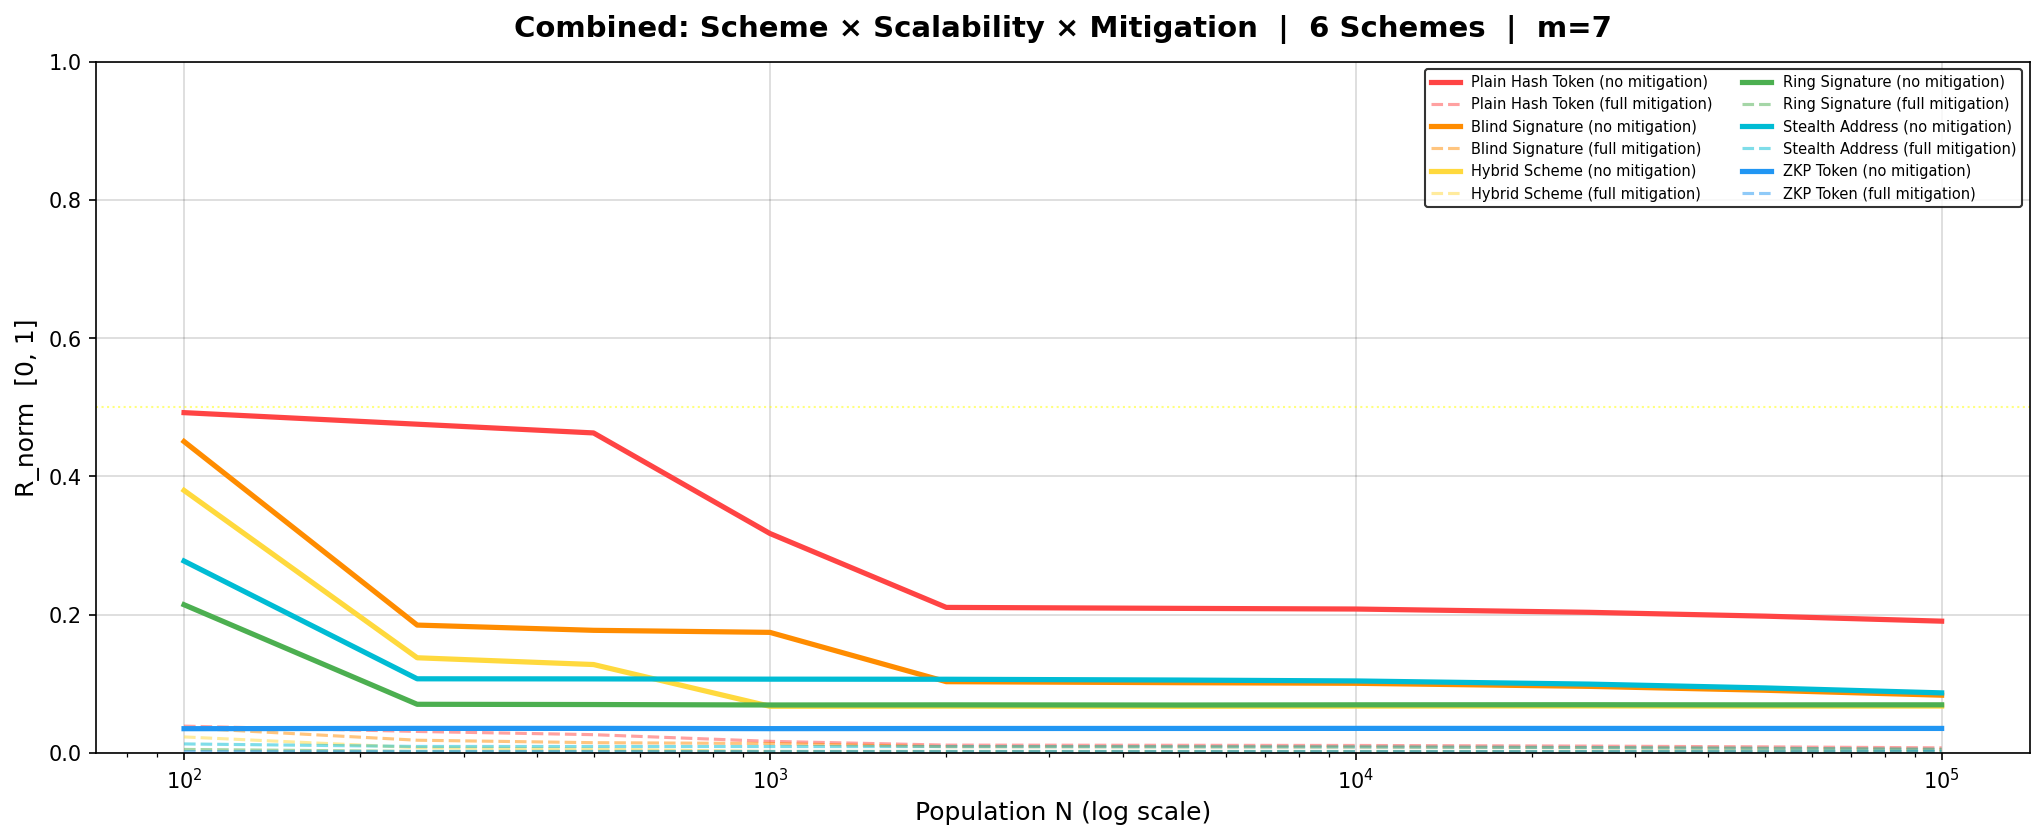
\includegraphics[width=\textwidth]{combined}
\caption{Combined view: $\Rnorm$ versus population size
for all six schemes. Solid lines = no mitigation. Dashed
lines = full mitigation stack. $m = 7$.}
\label{fig:combined}
\end{figure}

This combined view makes three findings visually
simultaneous. First, the risk ladder ordering is preserved
at every population size. Second, the full mitigation stack
compresses all schemes into a narrow band near $\Rnorm = 0$
regardless of baseline. Third, Plain Hash Token is the only
scheme that continues declining at $N = 100{,}000$ without
reaching a floor --- all other schemes have effectively
converged by that point. Together these three observations
confirm that cryptographic scheme selection, not population
scale or mitigation alone, is the primary determinant of
privacy risk in a token-based CBDC.
\chapter{Conclusions and Recommendations}
\label{ch:conclusions}

This chapter synthesises the findings of the thesis, provides
direct answers to the research questions stated in
Chapter~\ref{ch:introduction}, summarises the contributions of
the work, presents specific recommendations for the Nepal Rastra
Bank, and identifies directions for future research.

% ================================================================
\section{Summary of Work}
\label{sec:summary}
% ================================================================

This thesis developed a formal, normalised metadata
de-anonymization risk model for token-based Central Bank Digital
Currency and applied it to Nepal's domestic CBDC deployment
context under Nepal Rastra Bank jurisdiction.

The theoretical framework derived three interconnected components
from first principles. The single-attribute uniqueness score
$s(a_i)$ measures the fraction of users uniquely identifiable
from a single metadata attribute. The pairwise interaction
coefficient $\lambda_{ij}$ captures the amplification in
re-identification risk when two attributes are observed in
combination, beyond what either attribute reveals individually.
The normalised risk score $R_{\mathrm{norm}} = \Rraw / \Rmax$
maps total accumulated risk into the unit interval using a proven
theoretical upper bound $\Rmax(m) = m + \binom{m}{2}$, enabling
direct comparison across schemes, attribute sets, and population
sizes.

The model was applied to six cryptographic schemes --- Plain Hash
Token, Blind Signature, Hybrid Scheme, Ring Signature, Stealth
Address, and ZKP Token --- across seven metadata attributes
including two Nepal-specific fields: payment channel and
transaction zone. Eight analyses were conducted covering baseline
scheme comparison, population scalability, mitigation
effectiveness, attribute sensitivity, seed sensitivity,
micro-scale pilot behaviour, lambda sensitivity, and worst-case
calibration against the theoretical maximum.

% ================================================================
\section{Answers to Research Questions}
\label{sec:answers}
% ================================================================

\textbf{Primary question:} How can the metadata de-anonymization
risk of different cryptographic schemes in a token-based CBDC be
formally measured, normalised, and compared on a common
quantitative scale?

The $\Rnorm$ metric answers this question directly. By
normalising $\Rraw$ against its proven theoretical maximum
$\Rmax(m)$, the metric produces a scale-independent score in
$[0, 1]$ comparable across any number of attributes and any
population size. The metric was validated across 30 random seeds
and calibrated against a worst-case scenario achieving
$\Rnorm = 0.9994$, confirming the normalisation is correctly
calibrated at 99.9\% of the theoretical maximum.

\textbf{Secondary question 1 --- Scheme comparison:}
At baseline ($N = 1{,}000$, $m = 7$), the six schemes produce
the following $\Rnorm$ values: Plain Hash Token 0.317, Blind
Signature 0.174, Stealth Address 0.107, Ring Signature 0.069,
Hybrid Scheme 0.067, and ZKP Token 0.035. The six schemes form
a clean, non-overlapping risk ladder. ZKP Token is 9.1 times
safer than Plain Hash Token. Hybrid Scheme and Ring Signature
are statistically equivalent at $N = 1{,}000$.

\textbf{Secondary question 2 --- Population scalability:}
Scale does not resolve the privacy problem for weak schemes.
Plain Hash Token at $N = 100{,}000$ carries $\Rnorm = 0.191$
--- 5.5 times the risk of ZKP Token at the same scale. ZKP Token
is the only scheme whose $\Rnorm$ is scale-independent, remaining
flat at 0.035 from $N = 100$ to $N = 100{,}000$. This formally
disproves the assumption that population growth can substitute
for cryptographic privacy design.

\textbf{Secondary question 3 --- Mitigation effectiveness:}
A full mitigation stack reduces risk substantially across all
schemes. Ring Signature with full mitigation reaches
$\Rnorm = 0.002$, within 0.001 of ZKP Token with full mitigation.
Wallet unlinkability is the single most effective individual
mitigation across all schemes. Nepal Controls alone produce zero
risk reduction at $N = 1{,}000$ because Nepal's demographic
clustering already suppresses uniqueness on payment channel and
transaction zone.

\textbf{Secondary question 4 --- Nepal-specific context:}
Adding Nepal-specific attributes counterintuitively
\textit{decreases} $\Rnorm$ for all schemes because $\Rmax$
grows by 6 then 7 as each attribute is added, while $\Rraw$
increases by near-zero due to the skewed distributions of these
attributes. This formally proves that Nepal's demographic
structure provides passive privacy protection on payment channel
and transaction zone fields that does not require explicit
technical mitigation at domestic scale.

% ================================================================
\section{Contributions}
\label{sec:contributions}
% ================================================================

This thesis makes five contributions to the existing body of
knowledge.

\textbf{Contribution 1 --- Formal normalised privacy risk metric.}
The $\Rnorm$ metric provides the first formally derived,
normalised privacy risk score for token-based CBDC metadata.
Unlike k-anonymity and differential privacy, which were not
designed for scheme comparison, $\Rnorm$ produces a continuous
score in $[0, 1]$ directly comparable across any cryptographic
scheme, attribute set, and population size. The derivation of
$\Rmax(m) = m + \binom{m}{2}$ as the proven theoretical upper
bound is an original mathematical contribution.

\textbf{Contribution 2 --- Quantitative six-scheme comparison.}
This thesis provides the first quantitative comparison of six
CBDC cryptographic schemes on a common privacy risk metric. Prior
to this work, inter-scheme comparisons were qualitative. The risk
ladder spanning $\Rnorm = 0.317$ to $\Rnorm = 0.035$ gives
policymakers specific numbers for the privacy cost of each design
choice.

\textbf{Contribution 3 --- Formal disproof of scale substitution.}
The population scalability analysis formally disproves the
assumption that deploying a CBDC across a larger population
provides meaningful privacy improvement for weak schemes. Plain
Hash Token's residual risk floor of 0.191 at $N = 100{,}000$
demonstrates that cryptographic design, not population size, is
the determinant of long-run privacy risk.

\textbf{Contribution 4 --- Nepal-specific deployment analysis.}
By incorporating payment channel and transaction zone as
Nepal-specific attributes grounded in Nepal's payment
infrastructure, this thesis provides the first formal privacy risk
analysis specifically designed for Nepal's domestic CBDC context.

\textbf{Contribution 5 --- Micro-scale pilot risk quantification.}
The micro-scale analysis demonstrates that at VDC pilot scale
($N = 50$), all schemes except ZKP Token exceed
$\Rnorm = 0.48$. This finding directly informs how NRB should
approach any community-level CBDC pilot.

% ================================================================
\section{Recommendations for Nepal Rastra Bank}
\label{sec:nrb_recommendations}
% ================================================================

Based on the findings of this thesis, the following specific
recommendations are made to the Nepal Rastra Bank.

\textbf{Recommendation 1 --- Do not deploy Plain Hash Token at
any scale.} Plain Hash Token produces $\Rnorm = 0.317$ at pilot
scale and 0.191 at national scale. Both values represent
unacceptable citizen re-identification risk under Nepal's
constitutional right to privacy. The scheme should be excluded
from all deployment consideration.

\textbf{Recommendation 2 --- Adopt Ring Signature as the minimum
acceptable scheme for national deployment.} Ring Signature
achieves $\Rnorm = 0.069$ at baseline and 0.002 with a full
mitigation stack --- near-ZKP performance at significantly lower
computational cost.

\textbf{Recommendation 3 --- Consider Hybrid Scheme for
resource-constrained deployment.} Hybrid Scheme
($\Rnorm = 0.067$) is statistically equivalent to Ring Signature
($\Rnorm = 0.069$) at $N = 1{,}000$ and may be implementable at
lower computational cost on Nepal's low-end rural devices.

\textbf{Recommendation 4 --- Prioritise wallet unlinkability in
any mitigation stack.} Wallet unlinkability produces the largest
single reduction in $\Rnorm$ across all schemes. Any deployed
CBDC wallet should generate fresh addresses per transaction or
implement nullifier-based unlinkability.

\textbf{Recommendation 5 --- Do not rely on Nepal Controls as a
substitute for cryptographic privacy.} Nepal Controls produce
zero risk reduction at $N = 1{,}000$. Mitigation resources should
be focused on amount, timestamp, and wallet attributes where
marginal reduction is largest.

\textbf{Recommendation 6 --- Use ZKP Token only if computational
constraints can be resolved.} ZKP Token is the only scheme with
scale-independent risk. If NRB can resolve its computational
requirements through tiered CBDC architecture or offline ZKP
verification, it should be the target deployment scheme.

\textbf{Recommendation 7 --- Conduct any village pilot under
Ring Signature or better.} At $N = 50$, all schemes except ZKP
Token exceed $\Rnorm = 0.48$. Any NRB community-level pilot must
deploy Ring Signature or above to protect pilot participants from
high re-identification risk during the experimental phase.

% ================================================================
\section{Limitations}
\label{sec:limitations_ch5}
% ================================================================

The model uses synthetically generated transaction data rather
than real NRB records. While distributions are grounded in
Nepal's context, results may differ with real data having
different statistical properties.

The model captures pairwise interactions only. In datasets with
strong multi-way correlations the model may underestimate total
risk.

The adversary model covers passive observation only. Active
attacks are outside scope.

Several Hyperledger Fabric-specific metadata fields are not
modelled --- transaction ID linkability, endorsing peer identity,
and certificate metadata. Including these would increase $m$ and
likely increase $\Rnorm$ for all schemes.

% ================================================================
\section{Future Work}
\label{sec:future_work}
% ================================================================

\textbf{Higher-order interactions.} Extending the model to
triplet and higher-order interaction terms would increase
measurement precision for datasets with strong multi-way
correlations, generalising to $\binom{m}{k}$ terms for order $k$.

\textbf{Real transaction data.} Applying the model to real data
from eSewa, Khalti, or NRB's own records would validate the
synthetic distributions and produce deployment-specific estimates
directly actionable for NRB.

\textbf{Formal connection to existing frameworks.} A formal proof
connecting $\Rnorm$ to the k-anonymity framework of
\citet{sweeney2002} and the differential privacy framework of
\citet{dwork2006} would position the metric within the
established theoretical privacy literature.

\textbf{Additional Fabric metadata attributes.} Extending to
include transaction ID linkability, endorsing peer identity, and
certificate metadata would raise $m$ from 7 to approximately 10,
producing a more complete risk assessment for real Fabric
deployments.

\textbf{Cross-border remittance extension.} Including remittance
corridor in a cross-border CBDC model would address Nepal's
significant international financial flows excluded from this
domestic-scope analysis.

% ================================================================
\section{Closing Remarks}
\label{sec:closing}
% ================================================================

Nepal is at a consequential moment in its financial history.
Millions of citizens who have never held a bank account may soon
transact digitally for the first time. That opportunity is real,
but so is the risk that the systems built to serve them could
expose their lives in ways they never consented to.

The choice of cryptographic scheme in a CBDC is not a technical
detail. It is a policy decision with direct consequences for
every person who uses the system. The difference between Plain
Hash Token and Ring Signature is a factor of 4.6 in
re-identification risk at national scale. The difference between
Ring Signature with full mitigation and no mitigation is a
factor of 34.

Privacy in a CBDC is not incompatible with financial inclusion,
regulatory compliance, or operational efficiency. Ring Signature
with a full mitigation stack delivers near-ZKP privacy at a
fraction of ZKP's computational cost. Nepal does not have to
choose between reaching its unbanked population and protecting
that population's privacy. It has to choose the right
cryptographic scheme.
\newpage
\addcontentsline{toc}{chapter}{References}
\bibliography{references}
\def\appendixname{Annex}
\appendix
\chapter{Python Source Code}
\label{app:a_code}

The complete Python implementation is provided below.
The file \texttt{cbdc\_nepal\_final.py} produces all
results and charts in Chapter~\ref{ch:results}.

% Temporarily disabled - Python file has encoding issues
% \lstinputlisting[
%   language=Python,
%   basicstyle=\ttfamilyfootnotesize,
%   numbers=left,
%   numberstyle=\tiny\color{gray},
%   breaklines=true,
%   frame=single
% ]{annexes/cbdc_nepal_final.py}

See attached Python file for complete implementation.
You can find the source code for the full implementation of the project here:
\href{https://github.com/lioninthewild/thesis/blob/main/cbdc_nepal_final.py}%
{https://github.com/lioninthewild/thesis/blob/main/cbdc\_nepal\_final.py}
\end{document}